% Options for packages loaded elsewhere
\PassOptionsToPackage{unicode}{hyperref}
\PassOptionsToPackage{hyphens}{url}
%
\documentclass[
]{book}
\usepackage{amsmath,amssymb}
\usepackage{iftex}
\ifPDFTeX
  \usepackage[T1]{fontenc}
  \usepackage[utf8]{inputenc}
  \usepackage{textcomp} % provide euro and other symbols
\else % if luatex or xetex
  \usepackage{unicode-math} % this also loads fontspec
  \defaultfontfeatures{Scale=MatchLowercase}
  \defaultfontfeatures[\rmfamily]{Ligatures=TeX,Scale=1}
\fi
\usepackage{lmodern}
\ifPDFTeX\else
  % xetex/luatex font selection
  \setmainfont[]{Lucida Handwriting}
\fi
% Use upquote if available, for straight quotes in verbatim environments
\IfFileExists{upquote.sty}{\usepackage{upquote}}{}
\IfFileExists{microtype.sty}{% use microtype if available
  \usepackage[]{microtype}
  \UseMicrotypeSet[protrusion]{basicmath} % disable protrusion for tt fonts
}{}
\makeatletter
\@ifundefined{KOMAClassName}{% if non-KOMA class
  \IfFileExists{parskip.sty}{%
    \usepackage{parskip}
  }{% else
    \setlength{\parindent}{0pt}
    \setlength{\parskip}{6pt plus 2pt minus 1pt}}
}{% if KOMA class
  \KOMAoptions{parskip=half}}
\makeatother
\usepackage{xcolor}
\usepackage{longtable,booktabs,array}
\usepackage{calc} % for calculating minipage widths
% Correct order of tables after \paragraph or \subparagraph
\usepackage{etoolbox}
\makeatletter
\patchcmd\longtable{\par}{\if@noskipsec\mbox{}\fi\par}{}{}
\makeatother
% Allow footnotes in longtable head/foot
\IfFileExists{footnotehyper.sty}{\usepackage{footnotehyper}}{\usepackage{footnote}}
\makesavenoteenv{longtable}
\usepackage{graphicx}
\makeatletter
\def\maxwidth{\ifdim\Gin@nat@width>\linewidth\linewidth\else\Gin@nat@width\fi}
\def\maxheight{\ifdim\Gin@nat@height>\textheight\textheight\else\Gin@nat@height\fi}
\makeatother
% Scale images if necessary, so that they will not overflow the page
% margins by default, and it is still possible to overwrite the defaults
% using explicit options in \includegraphics[width, height, ...]{}
\setkeys{Gin}{width=\maxwidth,height=\maxheight,keepaspectratio}
% Set default figure placement to htbp
\makeatletter
\def\fps@figure{htbp}
\makeatother
\setlength{\emergencystretch}{3em} % prevent overfull lines
\providecommand{\tightlist}{%
  \setlength{\itemsep}{0pt}\setlength{\parskip}{0pt}}
\setcounter{secnumdepth}{5}
\usepackage{booktabs}
\ifLuaTeX
  \usepackage{selnolig}  % disable illegal ligatures
\fi
\usepackage[]{natbib}
\bibliographystyle{apalike}
\usepackage{bookmark}
\IfFileExists{xurl.sty}{\usepackage{xurl}}{} % add URL line breaks if available
\urlstyle{same}
\hypersetup{
  pdftitle={An Introduction to Research Methods in Mass Media},
  pdfauthor={Alex P Leith},
  hidelinks,
  pdfcreator={LaTeX via pandoc}}

\title{An Introduction to Research Methods in Mass Media}
\author{Alex P Leith}
\date{2024-08-18}

\begin{document}
\maketitle

{
\setcounter{tocdepth}{1}
\tableofcontents
}
\chapter{Preface}\label{preface}

This textbook, \emph{An Introduction to Research Methods in Mass Media}, has been developed as an essential resource for students and researchers delving into the intricate world of mass media research. The journey of crafting this book was driven by a profound understanding of the unique challenges that mass communications scholars encounter when applying quantitative research methods within a rapidly evolving digital landscape.

The primary motivation behind this textbook is to provide a detailed, step-by-step guide that integrates traditional research methodologies with the powerful tools offered by modern statistical software like R and RStudio. As media continue to evolve, so too must the methods we use to study them. This textbook seeks to bridge the gap between established research techniques and contemporary analytical tools, ensuring that students are well-equipped to tackle complex research questions with precision and confidence.

The structure of this textbook is designed to facilitate both learning and application. It begins with foundational concepts in research, including the ethical considerations essential to conducting responsible and impactful studies. From there, it guides readers through the process of formulating research questions, designing studies, and collecting data. The latter chapters delve into the nuanced processes of data analysis, visualization, and the interpretation of results using R and RStudio. Special attention is given to emerging trends in media research, including ethical challenges posed by new media technologies.

\begin{figure}
\centering
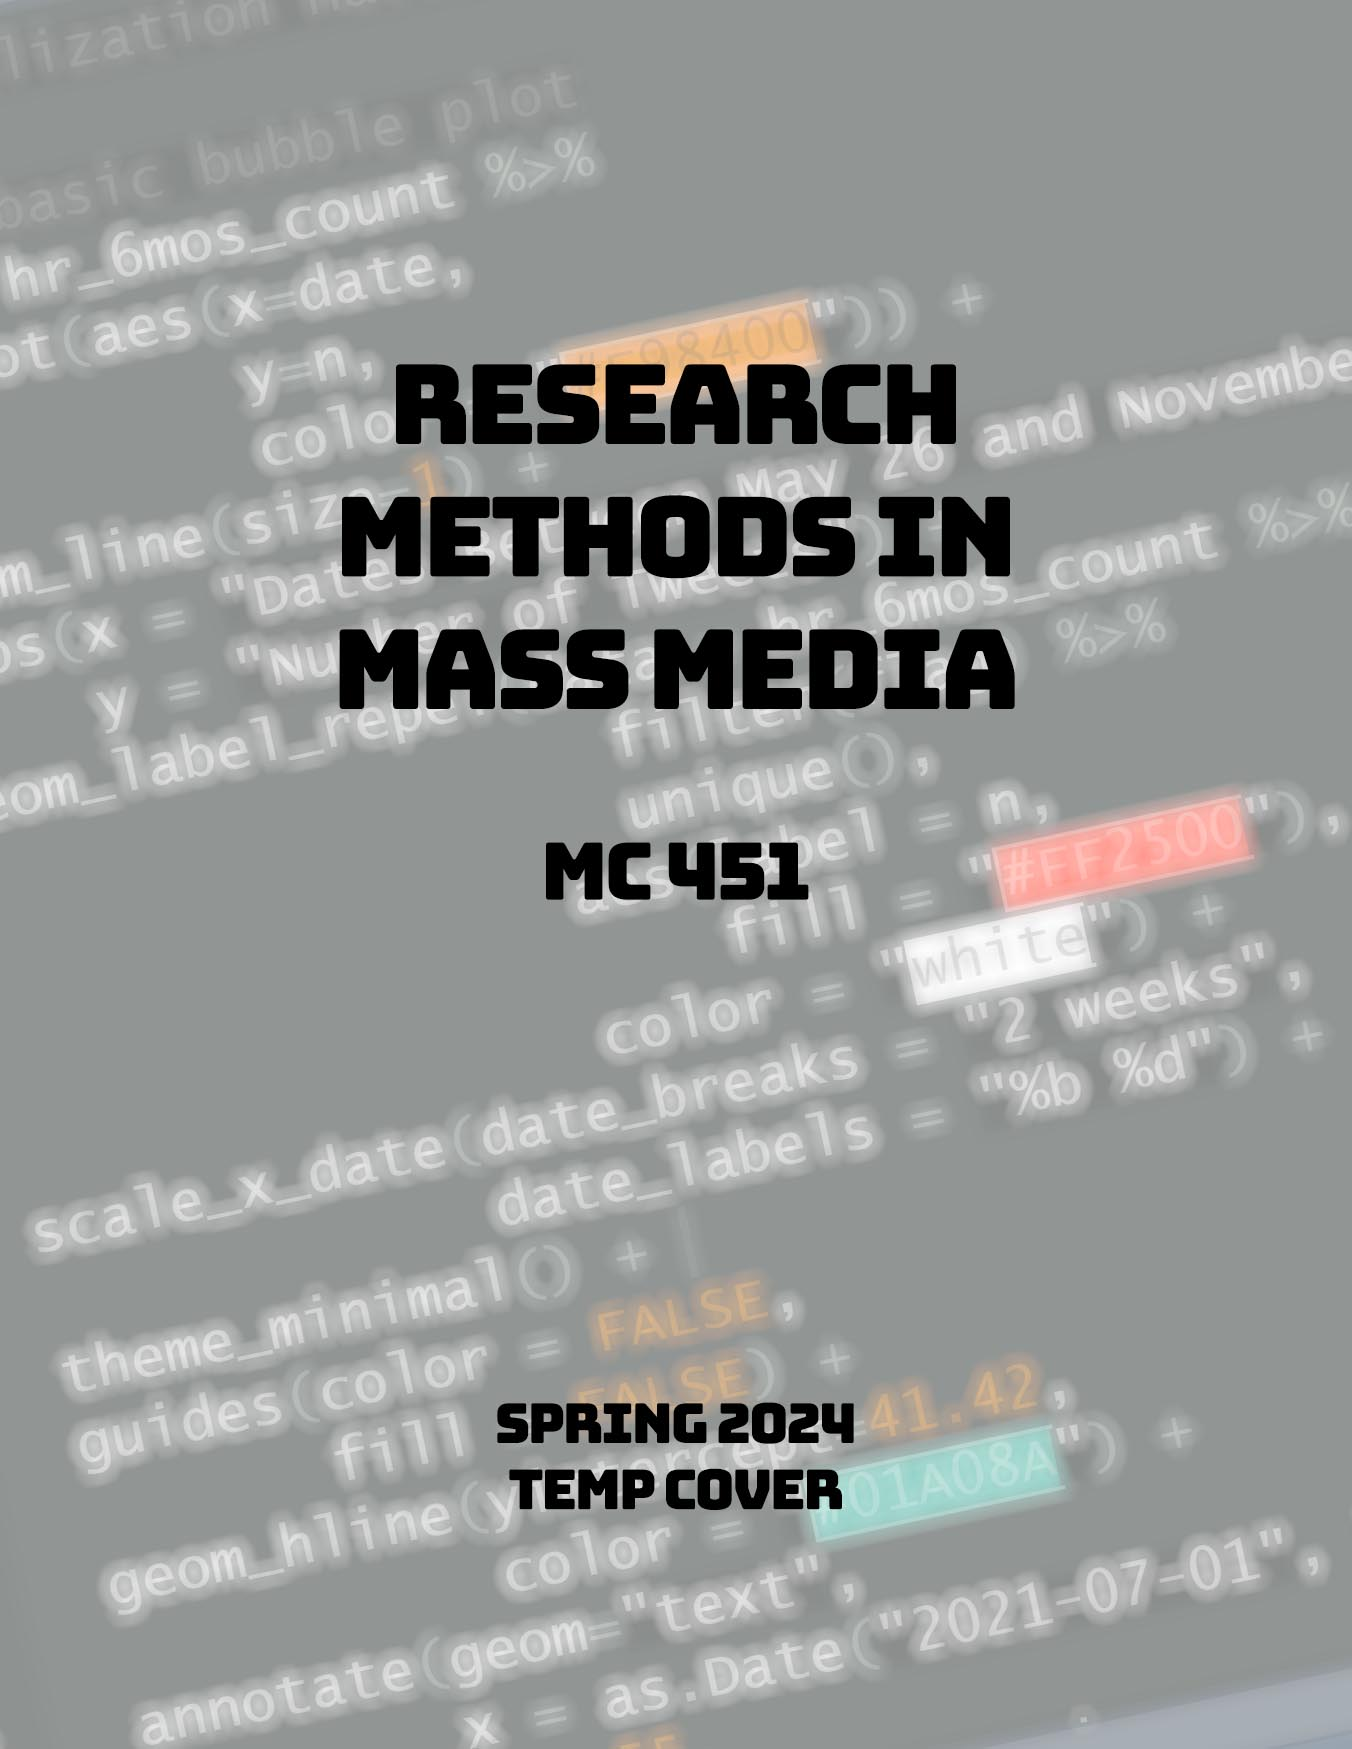
\includegraphics[width=1\textwidth,height=\textheight]{images/cover.jpg}
\caption{Temporary Cover}
\end{figure}

This book has been shaped by years of teaching, research, and practical experience in the field of mass communications. It reflects the insights gained from my work with students at Southern Illinois University Edwardsville and my ongoing research projects funded by organizations like the National Science Foundation. The examples and exercises included in the chapters are drawn from real-world scenarios, making the content both relevant and applicable to current research challenges.

I encourage readers to engage actively with the exercises, utilize the software tools provided, and critically think about how the research methods discussed can be applied to their own projects. The field of mass media research is dynamic, and this textbook is intended to be a living document that evolves alongside the media landscape. Feedback and insights from readers are not only welcome but essential for the continued refinement and relevance of this work.

I extend my gratitude to my colleagues, students, and the wider academic community whose contributions have enriched this textbook. I hope that this resource serves as a valuable guide and that it inspires rigorous, ethical, and innovative research in the field of mass communications.

\textbf{Licensing}

This book is published under a Creative Commons BY-SA license (CC BY-SA) version 4.0. This means that this book can be reused, remixed, retained, revised and redistributed (including commercially) as long as appropriate credit is given to the authors. If you remix, or modify the original version of this open textbook, you must redistribute all versions of this open textbook under the same license - CC BY-SA. \url{https://creativecommons.org/licenses/by-sa/4.0/}

\chapter{Introduction to Research in Mass Communications}\label{introduction-to-research-in-mass-communications}

\section{Overview of Research Methods}\label{overview-of-research-methods}

\subsection*{Definition and Importance of Research}\label{definition-and-importance-of-research}
\addcontentsline{toc}{subsection}{Definition and Importance of Research}

Research, in its most fundamental sense, is a systematic and methodical approach to inquiry. It involves the collection, analysis, and interpretation of data to answer specific questions or solve identified problems. In the realm of mass communications, research is not just a tool; it is the cornerstone of understanding the multifaceted interactions between media, individuals, and society. By delving into the intricate web of media influence, public opinion, and societal norms, researchers in mass communications can unravel the complexities that shape contemporary communication landscapes.

Mass communications research is vital for several reasons. First, it provides empirical evidence that can validate or refute theoretical frameworks within the field. This evidence-based approach ensures that the conclusions drawn are not based on conjecture or anecdotal observations but are grounded in systematic inquiry. For instance, through research, we can determine the extent to which media content influences public perceptions of social issues, thereby contributing to the development of more effective communication strategies.

Second, research in mass communications is crucial for identifying and analyzing trends in media production and consumption. Media environments are dynamic, with new platforms, technologies, and content forms continually emerging. Research enables scholars and practitioners to track these changes, understand their implications, and adapt accordingly. For example, the rise of social media has fundamentally altered how news is disseminated and consumed. Through research, we can explore how these changes impact traditional news media, audience engagement, and the broader public sphere.

\subsubsection*{Artifacts in Mass Communications Research}\label{artifacts-in-mass-communications-research}
\addcontentsline{toc}{subsubsection}{Artifacts in Mass Communications Research}

One of the key concepts in research is the use of \textbf{artifacts}. In the context of mass communications, artifacts are tangible or intangible objects, media, or representations that serve as primary sources of data in a study. These artifacts can take various forms, including newspaper articles, television broadcasts, social media posts, advertisements, films, and even digital content like podcasts or blogs. The selection and analysis of artifacts are critical to understanding the phenomena under investigation because they encapsulate the media's role in shaping societal discourse.

Artifacts are not merely objects of study; they are reflections of the socio-cultural environment in which they are produced. For instance, a researcher examining newspaper coverage of a political event is not only analyzing the content of the articles but also the underlying ideologies, biases, and power structures that influence how the event is reported. This broader perspective allows researchers to draw connections between media representations and societal attitudes, providing insights into how media can reinforce or challenge dominant narratives.

In analyzing artifacts, researchers often employ content analysis, a systematic coding and categorizing approach that allows for the quantification and examination of patterns within the media. Content analysis can be used to measure the frequency of specific themes, the portrayal of particular groups, or the use of specific language, among other attributes. By analyzing these patterns, researchers can make informed conclusions about the media's role in constructing social reality.

\subsubsection*{Attributes and Their Role in Research}\label{attributes-and-their-role-in-research}
\addcontentsline{toc}{subsubsection}{Attributes and Their Role in Research}

An \textbf{attribute} refers to any characteristic, feature, or quality that can be measured, observed, or coded within an artifact. Attributes are the building blocks of data in mass communications research, as they allow researchers to quantify and systematically analyze the elements that make up media content. Attributes can be both qualitative and quantitative, depending on the nature of the research question and the methodology employed.

For example, in a study analyzing the tone of news coverage, the tone (whether positive, neutral, or negative) is an attribute that can be systematically coded and analyzed across different articles. Other common attributes in media research include the frequency of certain words or phrases, the presence of specific images or symbols, the portrayal of gender roles, or the framing of particular issues. Attributes are essential because they provide a structured way to break down complex media content into manageable units of analysis.

\begin{figure}
\centering

\includegraphics[width=1\textwidth,height=\textheight]{images/fig01a.jpg}
\caption{Highlighting sentiment in newspaper}
\end{figure}

Attributes are not only used for descriptive analysis but also for inferential purposes. For instance, by comparing attributes across different media outlets, researchers can identify patterns of bias or differences in how issues are reported. This type of analysis is crucial for understanding the role of media in shaping public opinion and for assessing the diversity and plurality of perspectives presented in the media.

\subsubsection*{The Significance of Content Analysis}\label{the-significance-of-content-analysis}
\addcontentsline{toc}{subsubsection}{The Significance of Content Analysis}

\textbf{Content} in media research refers to the substance of communication, encompassing the messages, themes, narratives, and symbols conveyed through various media forms. Content analysis, one of the most widely used methods in mass communications research, involves the systematic examination of media content to uncover patterns, meanings, and implications.

Content analysis can be qualitative, focusing on the deeper meanings and interpretations of media messages, or quantitative, where the emphasis is on counting and measuring specific elements within the content. Both approaches are valuable, depending on the research objectives. For example, a qualitative content analysis might explore how narratives of heroism are constructed in wartime films, while a quantitative analysis might measure the frequency of different types of environmental issues covered in news broadcasts.

\begin{figure}
\centering
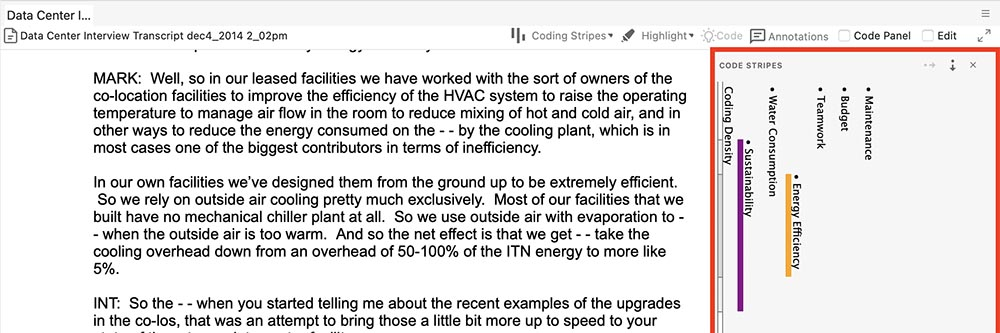
\includegraphics{images/fig01b.jpg}
\caption{Content analysis of interview using NVivo}
\end{figure}

The significance of content analysis lies in its ability to reveal the underlying messages and assumptions within media content. It allows researchers to move beyond surface-level descriptions to uncover the broader implications of media representations. For instance, by analyzing the content of political advertisements, researchers can assess how these ads influence voter behavior, contribute to political polarization, or reinforce gender stereotypes.

\subsubsection*{Studying Media Portrayals}\label{studying-media-portrayals}
\addcontentsline{toc}{subsubsection}{Studying Media Portrayals}

To illustrate the practical application of these concepts, consider a research project aimed at studying the portrayal of environmental issues in the media. In this study, the researcher might begin by selecting a set of news articles as artifacts. These articles serve as the primary data sources that will be systematically analyzed to address the research question.

The next step would involve identifying and coding the relevant attributes of these articles. For example, the researcher might code for the frequency of specific terms related to climate change, such as ``global warming,'' ``carbon emissions,'' or ``sustainability.'' The tone of the articles could also be coded as an attribute, with categories such as positive, neutral, or negative. Additionally, the researcher might analyze the framing of environmental issues, examining whether the articles emphasize the economic costs of addressing climate change or the moral imperative to act.

Once the artifacts and attributes have been coded, the researcher would analyze the content to uncover patterns and draw conclusions. For instance, the analysis might reveal that climate change is frequently framed as a distant, future problem rather than an immediate concern, potentially influencing public attitudes toward environmental policies. Alternatively, the analysis might show that certain news outlets consistently portray environmental activism in a negative light, contributing to public skepticism about environmental movements.

By engaging in this systematic analysis, researchers can generate insights that extend beyond the specific media content analyzed. They can contribute to broader discussions about media responsibility, public awareness, and the role of journalism in shaping societal values. Ultimately, research in mass communications serves as a critical tool for understanding the complex interactions between media and society, enabling us to make informed decisions about the media we consume and produce.

\subsection*{Qualitative vs.~Quantitative}\label{qualitative-vs.-quantitative}
\addcontentsline{toc}{subsection}{Qualitative vs.~Quantitative}

In mass communications research, understanding the distinction between qualitative and quantitative approaches is essential for grasping the breadth of methodologies available to scholars. These two primary approaches offer distinct pathways for exploring media messages, audience behaviors, and the societal impacts of communication. Each approach has its strengths, limitations, and appropriate applications, depending on the research question and the type of data being examined.

\subsubsection*{Qualitative Research}\label{qualitative-research}
\addcontentsline{toc}{subsubsection}{Qualitative Research}

\textbf{Qualitative research} is an interpretive approach that focuses on exploring the meaning, context, and complexity of media phenomena. This method is inherently flexible, allowing researchers to delve deeply into the nuances of how individuals and groups perceive, interpret, and experience media. Unlike quantitative research, which seeks to quantify and generalize findings across populations, qualitative research is concerned with understanding the rich, detailed, and often subjective aspects of communication.

One of the primary objectives of qualitative research is to uncover the underlying meanings and implications of media content. This approach is particularly well-suited for investigating complex or culturally specific phenomena that cannot be easily reduced to numerical data. For example, a qualitative study might explore how different cultural groups interpret a controversial advertisement, revealing the varying emotional responses, interpretations, and cultural references that inform their understanding of the ad.

Common methods used in qualitative research include in-depth interviews, focus groups, ethnography, and \textbf{content analysis}. In-depth interviews and focus groups involve direct interaction with participants, allowing researchers to gather detailed insights into their experiences and perspectives. Ethnography, on the other hand, involves the immersive study of media consumption within a specific cultural or social context, providing a holistic view of how media functions within that environment.

\textbf{Content analysis} in qualitative research involves the systematic examination of media content to identify patterns, themes, and implications. Unlike quantitative content analysis, which focuses on counting and categorizing content, qualitative content analysis aims to interpret the meaning behind the content. For example, a researcher might analyze the portrayal of gender roles in a series of television dramas, examining how these portrayals reinforce or challenge societal norms and expectations.

\textbf{Coding} is a crucial process in qualitative content analysis. It involves categorizing and organizing qualitative data into meaningful themes or groups, which helps researchers identify patterns and draw conclusions. Coding is an iterative process, often requiring multiple rounds of analysis as researchers refine their categories and interpretations. For instance, in analyzing a set of news articles, a researcher might initially code the content based on broad themes like ``political bias'' or ``framing of economic issues,'' and then further refine these codes to capture more specific patterns within the data.

The strengths of qualitative research lie in its ability to provide deep, contextualized insights into media phenomena. However, it also has limitations. The findings from qualitative studies are often specific to the context in which the research was conducted, making them difficult to generalize to broader populations. Additionally, qualitative research can be time-consuming and requires a high level of interpretive skill, as the researcher must navigate the complexities of subjective data.

\subsubsection*{Quantitative Research}\label{quantitative-research}
\addcontentsline{toc}{subsubsection}{Quantitative Research}

\textbf{Quantitative research} is a systematic approach that emphasizes the collection and analysis of numerical data. This method is grounded in the principles of objectivity and replicability, making it well-suited for studies that aim to measure the extent, frequency, or correlations of specific phenomena. Quantitative research is often used to test hypotheses, identify patterns, and establish causal relationships between variables.

In mass communications, quantitative research typically involves the use of surveys, experiments, and content analysis that quantifies aspects of media content. For example, a researcher might conduct a survey to measure the relationship between social media usage and political engagement among young adults. The survey results would provide numerical data that can be analyzed statistically to identify trends and correlations.

One of the key advantages of quantitative research is its ability to produce statistically significant results that can be generalized to larger populations. This generalizability is achieved through the use of random sampling and standardized data collection procedures, which help ensure that the findings are representative of the broader population. For instance, a nationwide survey on media consumption habits can provide insights into how different demographic groups engage with various media platforms, allowing researchers to draw conclusions about broader media trends.

\textbf{Experiments} are another common method in quantitative research. In an experimental study, researchers manipulate one or more variables to observe their effects on a dependent variable. This method is particularly useful for establishing causal relationships. For example, an experiment might examine the impact of violent video game exposure on aggressive behavior by randomly assigning participants to play either a violent or non-violent video game and then measuring their subsequent behavior.

Quantitative \textbf{content analysis} involves the systematic coding and counting of media content to identify patterns or trends. Unlike qualitative content analysis, which focuses on interpretation, quantitative content analysis seeks to quantify the presence of specific elements within the content. For example, a researcher might analyze a sample of news broadcasts to determine the frequency of negative versus positive coverage of a political candidate. The results of this analysis could then be used to assess media bias or the potential impact of news coverage on public opinion.

Despite its strengths, quantitative research also has limitations. The reliance on numerical data means that it may overlook the complexities and subtleties of human experience that are often captured in qualitative research. Additionally, while quantitative research can identify correlations between variables, it does not always provide insights into the underlying reasons or mechanisms behind these relationships.

\subsubsection*{Mixed Methods Approach}\label{mixed-methods-approach}
\addcontentsline{toc}{subsubsection}{Mixed Methods Approach}

In recognition of the complementary strengths of qualitative and quantitative research, many scholars in mass communications adopt a \textbf{mixed methods} approach. This approach combines the depth and context of qualitative research with the generalizability and rigor of quantitative research, providing a more comprehensive understanding of the research question.

A mixed methods study might begin with qualitative research to explore a phenomenon in depth, followed by quantitative research to measure its prevalence or test specific hypotheses. For example, a researcher might conduct in-depth interviews with social media users to understand their experiences with online harassment. The themes identified in these interviews could then inform the design of a survey that measures the prevalence of these experiences across a larger population. By integrating qualitative and quantitative data, the researcher can gain a richer and more nuanced understanding of the issue.

Mixed methods research is particularly valuable in mass communications, where the complexity of media phenomena often requires both detailed exploration and broad measurement. This approach allows researchers to address the limitations of each method, providing a more holistic view of the research topic.

\section{Research Ethics and the IRB Process}\label{research-ethics-and-the-irb-process}

\subsection*{Ethics in Research}\label{ethics-in-research}
\addcontentsline{toc}{subsection}{Ethics in Research}

Ethics in research serve as the guiding principles that ensure the integrity, respect, and fairness of the research process, especially in fields like mass communications, where studies often directly involve human participants. Ethical considerations are not just regulatory requirements but the bedrock upon which credible and responsible research is built. Researchers have a profound responsibility to protect the rights, dignity, and well-being of their participants while also ensuring the validity and trustworthiness of their findings. This section delves deeper into the key ethical principles that every researcher must understand and uphold: informed consent, confidentiality, and anonymity.

\subsubsection*{Informed Consent}\label{informed-consent}
\addcontentsline{toc}{subsubsection}{Informed Consent}

\textbf{Informed consent} is a fundamental ethical principle that involves providing potential participants with all necessary information about a study before they agree to take part. The concept of informed consent is rooted in the respect for the autonomy and agency of individuals, allowing them to make voluntary and informed decisions about their participation in research. This principle not only safeguards the rights of participants but also strengthens the ethical foundation of the research.

The process of obtaining informed consent goes beyond merely securing a signature on a consent form. It involves an ongoing dialogue between the researcher and the participant, where the researcher must ensure that the participant fully understands the purpose of the study, the procedures involved, any potential risks or benefits, and their rights as a participant. This communication must be clear, transparent, and tailored to the participant's level of comprehension. In cases where participants may have limited literacy or where the study involves complex procedures, additional measures such as verbal explanations or visual aids may be necessary to facilitate understanding.

\begin{figure}
\centering

\includegraphics{images/fig01c.jpg}
\caption{Informed consent template}
\end{figure}

Informed consent is especially critical in studies involving vulnerable populations, such as children, individuals with cognitive impairments, or those who may be in coercive situations. In such cases, researchers must take extra precautions to ensure that consent is genuinely informed and voluntary. This may involve seeking consent from a legal guardian or employing independent advocates to confirm that the participant's rights are fully protected.

The ethical importance of informed consent cannot be overstated. It serves as the foundation of the trust relationship between the researcher and the participant. Any breach of this trust, such as misleading participants about the nature of the study or failing to disclose potential risks, can have serious ethical and legal implications. Researchers must also recognize that informed consent is not a one-time event but a continuous process. Participants should have the opportunity to ask questions, seek clarification, and withdraw from the study at any point without facing any consequences.

\subsubsection*{Confidentiality}\label{confidentiality}
\addcontentsline{toc}{subsubsection}{Confidentiality}

\textbf{Confidentiality} is another cornerstone of ethical research, referring to the obligation of the researcher to protect the private information of participants. When participants agree to share personal or sensitive information, they do so with the expectation that this information will be kept secure and will not be disclosed to unauthorized parties. Upholding confidentiality is essential for maintaining the trust between researchers and participants and for ensuring that participants do not suffer harm as a result of their involvement in the research.

Confidentiality involves several key practices. Researchers must take proactive steps to ensure that data is stored securely, whether in physical form (e.g., locked filing cabinets) or digital form (e.g., encrypted databases). Access to this data should be restricted to authorized personnel only, and any sharing of data should be done with the participant's explicit consent and in a manner that does not compromise their privacy.

In some research contexts, particularly those involving sensitive topics such as mental health, political beliefs, or illegal behaviors, the potential risks of breaching confidentiality are heightened. A breach of confidentiality could lead to serious consequences for participants, including social stigma, legal repercussions, or psychological distress. For example, if a participant's involvement in a study about drug use were disclosed without their consent, they could face legal action or social ostracization. As such, researchers must be vigilant in their efforts to protect participant confidentiality.

Moreover, confidentiality extends beyond the immediate research team. When presenting findings or publishing research, researchers must anonymize data to prevent the identification of individual participants. This may involve aggregating data, using pseudonyms, or omitting specific details that could lead to the identification of participants. Ethical research reporting also requires that researchers be transparent about the measures they have taken to protect confidentiality and to discuss any limitations that may affect participant anonymity.

\subsubsection*{Anonymity}\label{anonymity}
\addcontentsline{toc}{subsubsection}{Anonymity}

\textbf{Anonymity} is closely related to confidentiality but goes a step further by ensuring that participants cannot be identified based on the data they provide. In truly anonymous studies, not even the researcher can link data to specific participants, providing an additional layer of privacy protection. Anonymity is particularly important in research involving sensitive or stigmatized issues, where participants might be reluctant to share honest responses if they fear being identified.

Achieving anonymity can be challenging, especially in qualitative research or studies that collect detailed personal data. Researchers must carefully design their studies to protect participant anonymity, which might involve using anonymous surveys, stripping identifying information from datasets, or employing techniques such as data masking or aggregation to ensure that individual participants cannot be singled out.

\begin{figure}
\centering

\includegraphics{images/fig01d.jpg}
\caption{Representation of anonymity during focus group study.}
\end{figure}

However, anonymity is not always feasible or desirable, depending on the nature of the study. For example, in longitudinal research where the same participants are studied over time, maintaining anonymity while tracking changes in individual responses can be difficult. In such cases, researchers must balance the need for data continuity with the ethical obligation to protect participants' privacy. When anonymity cannot be guaranteed, researchers must be transparent with participants about the level of privacy they can expect and must take all possible steps to mitigate risks.

Ensuring anonymity also requires careful consideration in the dissemination of research findings. Researchers must avoid including any details in their reports or publications that could inadvertently reveal the identity of participants. This is particularly relevant in case studies or research involving small, easily identifiable populations. Even seemingly innocuous details, such as a participant's occupation or location, could potentially compromise anonymity if the sample size is small or the population is well-known.

\subsubsection*{Ethical Challenges and Considerations}\label{ethical-challenges-and-considerations}
\addcontentsline{toc}{subsubsection}{Ethical Challenges and Considerations}

While the principles of informed consent, confidentiality, and anonymity are clear, their application in practice can be complex and fraught with challenges. Researchers must navigate these ethical considerations while also ensuring the scientific rigor and validity of their studies. For example, balancing the need for rich, detailed data with the obligation to protect participant anonymity can be particularly challenging in qualitative research.

Furthermore, ethical considerations extend beyond the immediate research process to include the dissemination and application of research findings. Researchers must consider the potential impact of their work on the participants, communities, and societies they study. This includes being mindful of how research findings might be interpreted, used, or misused, particularly in politically or socially sensitive contexts. Ethical research requires a commitment to minimizing harm and maximizing benefits not only for participants but for society as a whole.

Ethical dilemmas in research are often not black-and-white, and researchers may encounter situations where they must make difficult decisions about how best to uphold ethical principles. In such cases, consulting ethical guidelines, seeking advice from institutional review boards (IRBs), and engaging in ongoing ethical reflection are crucial steps in navigating these challenges.

\subsection*{Navigating the IRB Process}\label{navigating-the-irb-process}
\addcontentsline{toc}{subsection}{Navigating the IRB Process}

Navigating the Institutional Review Board (IRB) process is a critical component of conducting ethical research involving human participants. The IRB is responsible for reviewing research proposals to ensure that they comply with ethical standards and protect the rights and welfare of participants. As a researcher, particularly within the context of Southern Illinois University Edwardsville (SIUE), understanding the intricacies of this process is essential for gaining approval and conducting your research responsibly. This section will thoroughly explore the key components of the IRB process at SIUE, including creating consent forms, debriefing participants, assessing potential harm, offering incentives, and understanding the submission protocols.

\subsubsection*{Developing Consent Forms}\label{developing-consent-forms}
\addcontentsline{toc}{subsubsection}{Developing Consent Forms}

\textbf{Consent forms} are a cornerstone of ethical research, providing participants with all the necessary information to make an informed decision about their involvement in the study. At SIUE, the creation of a consent form must align with the ethical guidelines and requirements stipulated by the IRB. The consent form must clearly outline the study's purpose, procedures, potential risks, benefits, and the measures in place to ensure participant confidentiality.

Creating a consent form is more than just completing a document; it involves crafting a communication tool that genuinely informs participants. According to the SIUE guidelines, the language used in consent forms should be clear, concise, and devoid of technical jargon that might confuse participants (IRB Protocol Guidance, 2023). For example, when explaining complex procedures, it is crucial to break down the information into understandable segments, ensuring that participants fully comprehend what their participation entails.

Moreover, the consent form must explicitly state that participation is voluntary and that participants can withdraw from the study at any point without any negative consequences. This ensures that participants are not coerced or unduly influenced to continue their involvement against their will. The \textbf{2023 IRB Protocol Guidance} document from SIUE emphasizes that consent forms should include detailed information on how participants can withdraw and what steps will be taken to handle their data if they choose to do so (IRB Protocol Guidance, 2023).

\subsubsection*{The Debriefing Process}\label{the-debriefing-process}
\addcontentsline{toc}{subsubsection}{The Debriefing Process}

\textbf{Debriefing} is another crucial aspect of the IRB process, particularly in studies where deception is used or where participants might not be fully aware of the study's purpose during their involvement. Debriefing involves providing participants with a complete explanation of the study after their participation, ensuring they leave with a clear understanding of what the research was about and why certain methodologies, such as deception, were employed.

At SIUE, debriefing is especially important in research that involves sensitive topics or procedures that could cause distress. The debriefing process should be conducted in a manner that is sensitive to the participants' experiences during the study. It should include a thorough explanation of the study's true purpose, an overview of the participant's role, and an opportunity for participants to ask questions or express concerns. Additionally, researchers must provide contact information for follow-up questions and offer resources if the study touched on potentially distressing issues.

The \textbf{Research Participant Notification} document is a key tool in this process, as it provides participants with formal documentation about the study, their rights, and contact information for any follow-up questions (Research Participant Notification, 2023). Researchers must ensure that this document is provided and explained to participants during the debriefing session.

\subsubsection*{Assessing and Minimizing Harm}\label{assessing-and-minimizing-harm}
\addcontentsline{toc}{subsubsection}{Assessing and Minimizing Harm}

\textbf{Assessing potential harm} to participants is a fundamental responsibility when navigating the IRB process. Harm can manifest in various forms, including physical discomfort, psychological distress, or social risks such as breaches of confidentiality. The IRB at SIUE requires that researchers conduct a thorough risk assessment as part of their protocol submission, outlining any potential risks and the measures that will be taken to mitigate them.

When assessing harm, researchers must consider both the likelihood and the severity of potential risks. For instance, a study involving interviews about traumatic experiences must account for the psychological impact of recalling such events on participants. The protocol must detail how these risks will be minimized, such as by providing access to counseling services or by designing interview questions that are sensitive to the participants' emotional state.

The \textbf{Protocols} document highlights the importance of a detailed risk-benefit analysis, where researchers must justify that the potential benefits of the research outweigh any identified risks (Protocols, 2024). This analysis is crucial for IRB approval, as the board will scrutinize whether the proposed protections are sufficient and appropriate given the nature of the study.

\subsubsection*{Offering Incentives}\label{offering-incentives}
\addcontentsline{toc}{subsubsection}{Offering Incentives}

\textbf{Incentives} can play a significant role in participant recruitment and retention, but they must be carefully managed to avoid coercion. The IRB at SIUE requires that any incentives offered to participants be proportional to the time and effort required and not so large that they unduly influence participation, especially in studies involving any level of risk.

Incentives should be described in the IRB protocol submission, with a clear justification of why the chosen incentive is appropriate. For example, offering a small gift card or a modest monetary payment is generally acceptable, but offering a large sum of money might be considered coercive, particularly in studies involving vulnerable populations. The \textbf{IRB Protocol Guidance} document advises researchers to carefully consider the ethical implications of incentives and to ensure that they do not overshadow the voluntary nature of participation (IRB Protocol Guidance, 2023).

\begin{figure}
\centering

\includegraphics{images/fig01e.jpg}
\caption{Example of an excessive cash incentive}
\end{figure}

The \textbf{Recruitment Document} provided by SIUE serves as a template for informing potential participants about the study and any incentives they might receive (IRB Recruitment Document, 2023). It is essential to update this document with specific details relevant to your study and ensure that the incentives are described transparently.

\subsubsection*{Submission and Review Protocols}\label{submission-and-review-protocols}
\addcontentsline{toc}{subsubsection}{Submission and Review Protocols}

Navigating the IRB process at SIUE requires careful attention to detail in the submission and review stages. The IRB submission protocol involves several key steps, beginning with the completion of the IRB application in the Kuali system. Researchers must ensure that all sections of the protocol are thoroughly completed, including detailed descriptions of the research methods, participant recruitment strategies, and data management plans.

The \textbf{Protocols} document emphasizes the importance of thoroughly reading and responding to each question in the IRB submission, as incomplete or vague answers can lead to delays in the review process (Protocols, 2024). Researchers are encouraged to submit their protocols well in advance of the anticipated start date to allow sufficient time for review and any necessary revisions.

Additionally, all student-led research at SIUE requires a faculty advisor's approval and signature, confirming that the student has a solid understanding of the ethical guidelines and that the study is methodologically sound (Faculty Advisor Signature, 2024). This step is crucial for ensuring that the research meets the university's standards and adheres to all ethical requirements.

The IRB review can fall into different categories, such as exempt, expedited, or full board review, depending on the nature of the study. Each category has specific requirements and timelines, and researchers must select the appropriate category based on their study's characteristics. The \textbf{IRB Protocol Guidance} document provides detailed instructions on how to determine the correct review category and what each entails (IRB Protocol Guidance, 2023).

\subsection*{Ethical Considerations Specific to Mass Media Research}\label{ethical-considerations-specific-to-mass-media-research}
\addcontentsline{toc}{subsection}{Ethical Considerations Specific to Mass Media Research}

When conducting research in mass media, researchers must navigate unique ethical considerations that arise from the specific nature of this field. Unlike other disciplines, mass media research often involves observing and interacting with individuals in their natural environments, such as during their routine media consumption or within online communities. This approach brings forth specific challenges, particularly related to the \textbf{observer effect} and the role of the \textbf{observer-as-participant}. These concepts are crucial for understanding the potential influence a researcher can have on the subjects being studied and for ensuring the ethical integrity of the research process.

\subsubsection*{The Observer Effect}\label{the-observer-effect}
\addcontentsline{toc}{subsubsection}{The Observer Effect}

The \textbf{observer effect} refers to the phenomenon where the mere presence of a researcher can alter the behavior of the individuals being observed. This effect is particularly significant in mass media research, where participants' media consumption habits or online activities might change if they are aware of being monitored. For example, if individuals know that their social media activity is under observation, they may modify their behavior, perhaps by avoiding controversial content or engaging more carefully in discussions, leading to results that do not accurately reflect their typical behavior.

The observer effect presents a considerable challenge for researchers aiming to capture authentic data. If the participants alter their behavior due to the awareness of being observed, the data collected may be skewed, leading to conclusions that are not truly representative of the subject's usual actions. This can compromise the validity of the research, making it difficult to draw accurate conclusions about media consumption patterns, audience behavior, or the effects of media content.

To mitigate the observer effect, researchers can employ \textbf{unobtrusive measures}---techniques that allow data collection without directly interacting with or influencing the subjects. For instance, researchers might analyze publicly available online data where participants are unaware of the specific focus of the study. However, this approach must be balanced with ethical considerations, particularly regarding the privacy of individuals and the potential implications of observing people without their explicit consent. Even when using unobtrusive measures, researchers must remain vigilant about the ethical implications, especially when dealing with sensitive topics or vulnerable populations.

\subsubsection*{The Observer-as-Participant Role}\label{the-observer-as-participant-role}
\addcontentsline{toc}{subsubsection}{The Observer-as-Participant Role}

The \textbf{observer-as-participant} role is another critical concept in mass media research, where the researcher not only observes the subjects but also actively engages with them. This dual role can provide valuable insights by allowing the researcher to experience the environment from within, gaining a deeper understanding of the social dynamics, cultural norms, and interactions that influence media consumption and behavior.

For example, a researcher studying online communities might participate in discussions, share content, and interact with community members to better understand how these interactions shape media consumption patterns and influence group behavior. This approach can offer a rich, nuanced perspective that is difficult to achieve through observation alone.

\begin{figure}
\centering
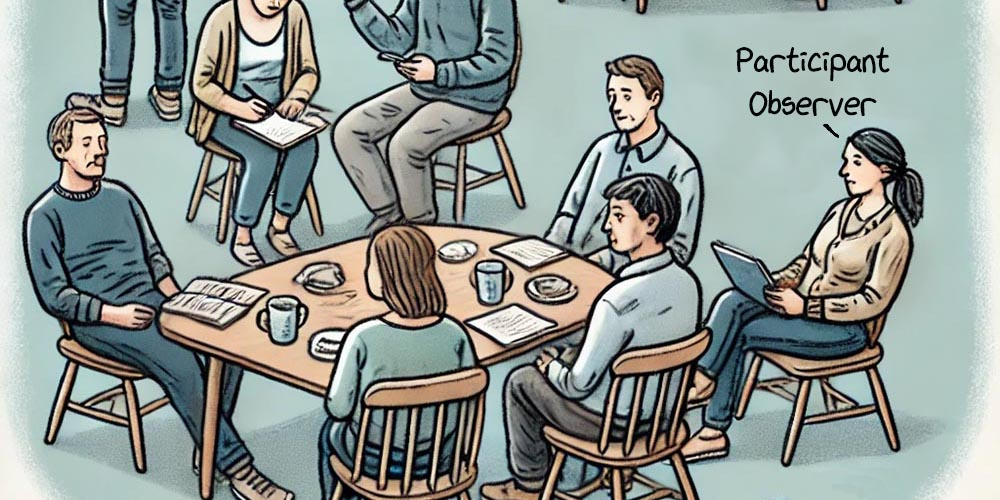
\includegraphics{images/fig01f.jpg}
\caption{Representation of participant observer}
\end{figure}

However, the observer-as-participant role also introduces significant ethical challenges. The researcher's involvement in the community can influence the very behavior they aim to study, potentially leading to biased results. Moreover, there is the risk of compromising objectivity, as the researcher becomes part of the social fabric they are studying. Transparency is crucial in this role; researchers must clearly disclose their identity and purpose to the subjects, ensuring that their interactions do not mislead or manipulate the community. Ethical dilemmas can arise if the researcher's participation changes the dynamics of the group or if their influence leads to outcomes that would not have occurred naturally.

Maintaining a balance between active participation and objective observation is essential but challenging. Researchers must constantly reflect on their role and the potential impact of their actions, taking care not to distort the data or influence the subjects more than necessary. In some cases, researchers may need to withdraw from active participation to ensure that their presence does not overly affect the behavior of the subjects.

\subsubsection*{Ethical Considerations and Strategies for Mitigation}\label{ethical-considerations-and-strategies-for-mitigation}
\addcontentsline{toc}{subsubsection}{Ethical Considerations and Strategies for Mitigation}

Both the observer effect and the observer-as-participant role highlight the ethical complexities involved in mass media research. Researchers must carefully consider how their presence and actions might influence the subjects and the data being collected. To address these challenges, several strategies can be employed:

\begin{enumerate}
\def\labelenumi{\arabic{enumi}.}
\item
  \textbf{Transparency}: Being transparent with participants about the research objectives and the researcher's role can help mitigate ethical concerns. This includes clear communication about the nature of the study, the role of the researcher, and the ways in which data will be collected and used.
\item
  \textbf{Informed Consent}: When feasible, obtaining informed consent from participants is crucial, particularly when the research involves direct interaction or observation. This ensures that participants are aware of the study and have agreed to be part of it, which can help mitigate the observer effect.
\item
  \textbf{Minimizing Interaction}: In cases where the observer effect might significantly alter participant behavior, researchers should consider minimizing their interaction with the subjects. This can be achieved through techniques such as passive observation, using anonymized data, or relying on existing data sets that do not involve real-time interaction.
\item
  \textbf{Ethical Reflection}: Researchers must engage in continuous ethical reflection, considering the potential impacts of their research on the subjects and the community. This involves evaluating the risks and benefits of the research, seeking advice from ethical review boards, and being prepared to adjust the research approach if ethical concerns arise.
\item
  \textbf{Balancing Roles}: When adopting the observer-as-participant role, researchers should carefully balance their involvement with the need to maintain objectivity. This might involve setting clear boundaries for participation and regularly reviewing the impact of their presence on the group dynamics.
\end{enumerate}

\chapter{Developing Research Questions and Hypotheses}\label{developing-research-questions-and-hypotheses}

\section{Formulating Research Questions}\label{formulating-research-questions}

\subsection{Conceptual Definitions and Operationalization}\label{conceptual-definitions-and-operationalization}

In mass media research, it is essential to understand the difference between conceptual definitions and operationalization. These two processes form the foundation of how we study and measure abstract phenomena. By clearly defining concepts and determining how they will be measured, researchers can ensure that their studies are both rigorous and meaningful.

Let's start by discussing the idea of a \textbf{concept}. A concept is an abstract idea that represents a phenomenon you are interested in studying. Concepts are the building blocks of research, helping us to focus our inquiry on specific aspects of reality. For example, consider the concept of ``media influence.'' This is a broad idea that could encompass many different types of influence, such as how media shapes public opinion, affects individual behavior, or reinforces cultural norms. Similarly, ``audience engagement'' is another concept that might refer to how actively people participate in media consumption, interact with content, or share it with others.

To better understand how concepts are used in research, it's helpful to begin with a broad example. Take the concept of ``democracy.'' Democracy is an abstract idea that can be explored from various angles, such as political participation, freedom of speech, or electoral processes. In research, defining this concept more narrowly allows us to study specific aspects of democracy, such as voter turnout or the impact of media on political knowledge. By narrowing down broad concepts into more specific definitions, researchers can focus their studies and make their findings more relevant and actionable.

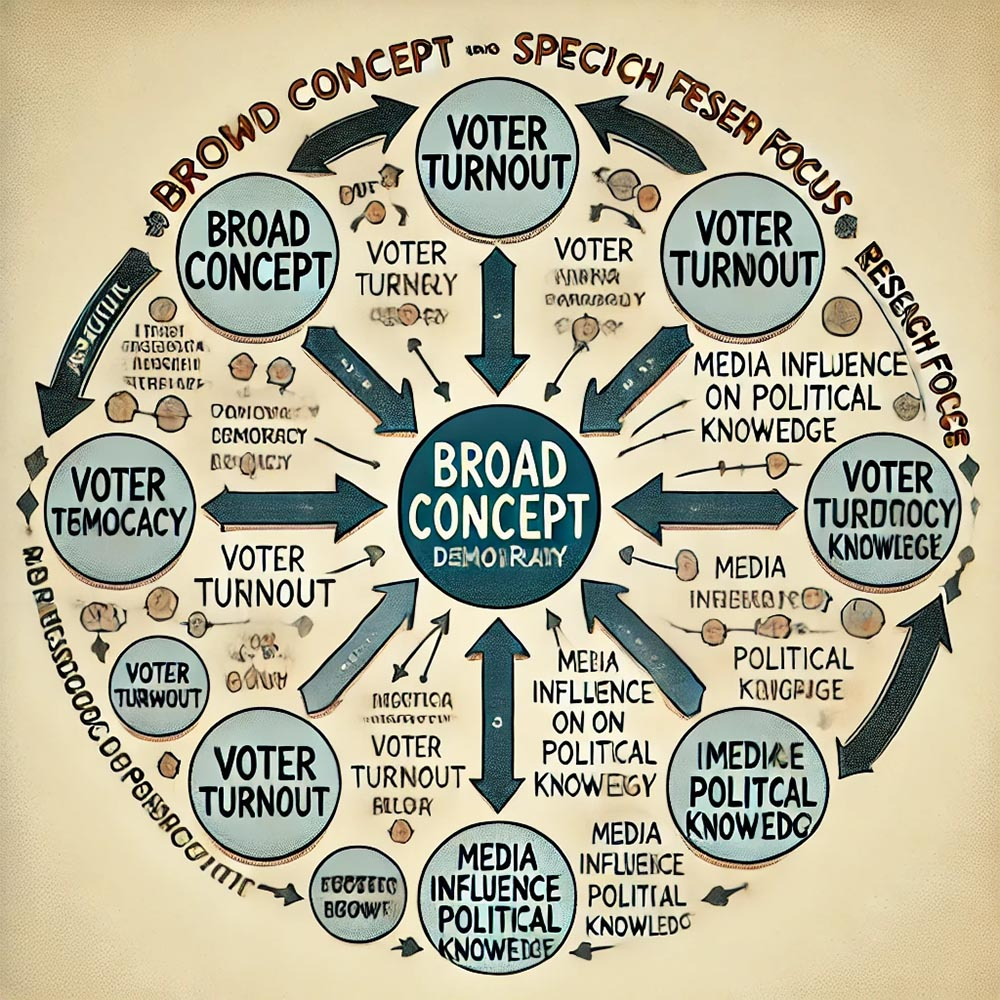
\includegraphics[width=1\textwidth,height=\textheight]{images/fig013.jpg}

\emph{Figure 013. A visual representation of the process of narrowing a broad concept into a specific research focus. The image could start with a large circle labeled ``Broad Concept'' (e.g., ``Democracy'') and show arrows pointing to smaller circles with more focused aspects (e.g., ``Voter Turnout,'' ``Media Influence on Political Knowledge''). This image would help students visualize how broad ideas are refined into researchable topics.}

Once you have a clear concept in mind, the next step is \textbf{operationalization}, which is the process of defining how that concept will be measured in your study. Operationalization involves taking an abstract concept and turning it into something that can be observed and quantified. This step is crucial because it bridges the gap between theory and empirical research, allowing you to gather data that can be analyzed and interpreted.

For instance, if you are studying ``audience engagement,'' you need to determine how to measure this concept in a way that reflects its true meaning. One way to operationalize audience engagement might be to look at social media metrics, such as the number of likes, shares, and comments a piece of content receives. These metrics provide tangible data that can be used to assess how engaged an audience is with a particular media message. Similarly, if you were studying ``media influence,'' you might operationalize this concept by measuring changes in public opinion before and after exposure to a specific media campaign.

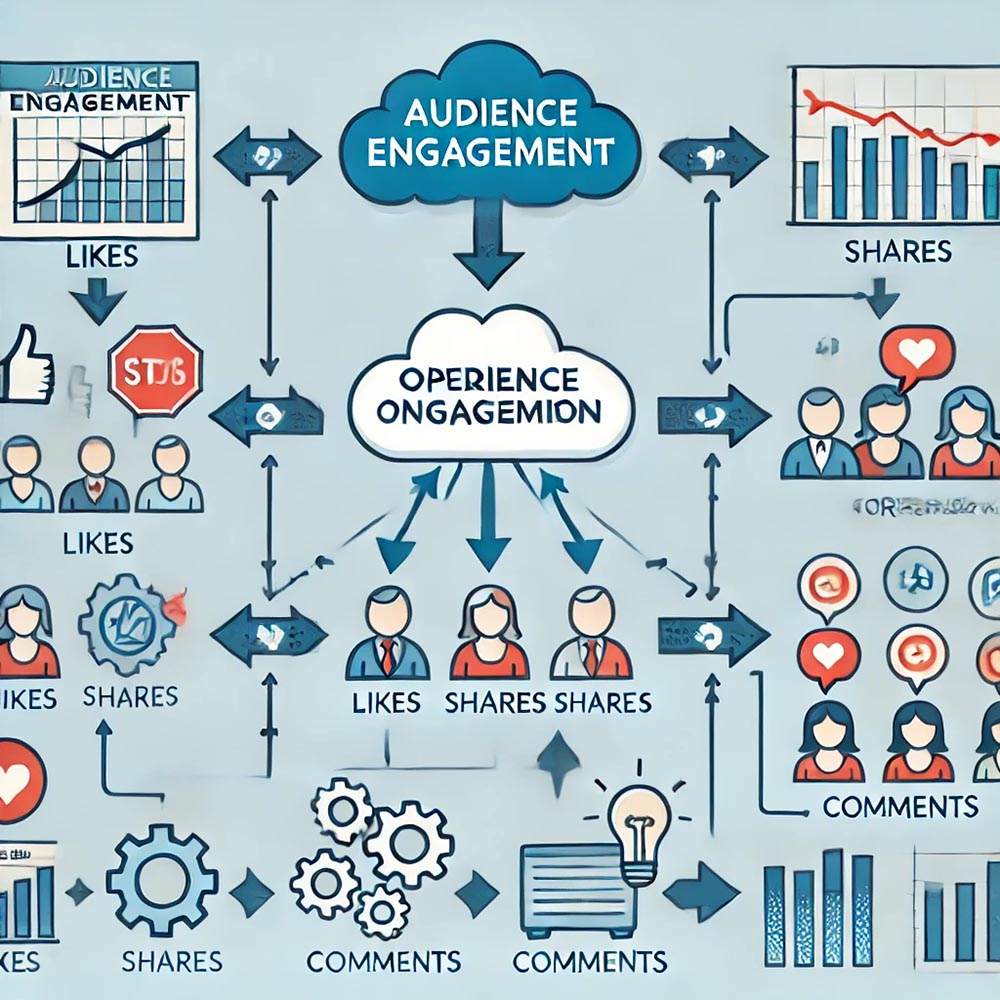
\includegraphics[width=1\textwidth,height=\textheight]{images/fig014.jpg}

\emph{Figure 014. A step-by-step flowchart illustrating the operationalization process. The image could begin with an abstract concept (e.g., ``Audience Engagement''), followed by arrows pointing to specific measurable variables (e.g., ``Likes,'' ``Shares,'' ``Comments''). The final step could show these variables being analyzed in a research context. This visual would help students understand how abstract ideas are translated into measurable data.}

To deepen your understanding of these processes, we will begin by exploring examples of broad concepts and discussing how they can be used in research. For instance, we might start with the concept of ``public opinion'' and examine how it can be studied through various lenses, such as survey data, media analysis, or behavioral observation. This will help you see how researchers define their concepts and why these definitions are critical for conducting meaningful research.

Next, we will engage in a brainstorming session where you will identify concepts relevant to mass media that interest you. This collaborative activity will allow you to explore different ideas and discuss their meanings and significance with your peers. By the end of this session, you should have a clearer idea of how to articulate your research interests in the form of well-defined concepts.

Following this, we will focus on operationalization, using case studies to illustrate how abstract concepts are transformed into measurable variables. For example, we might look at a study that operationalizes ``political participation'' by measuring voter registration rates, attendance at political rallies, or participation in online political discussions. By analyzing these case studies, you will learn how researchers make decisions about which variables best capture the essence of the concept they are studying.

Finally, you will have the opportunity to practice creating operational definitions for a list of given concepts. This exercise will challenge you to think critically about how to measure abstract ideas in a way that is both accurate and meaningful. You might, for example, be asked to operationalize the concept of ``media literacy'' by deciding which behaviors or knowledge indicators best represent this idea. Through this practice, you will develop the skills needed to turn theoretical concepts into practical research tools.

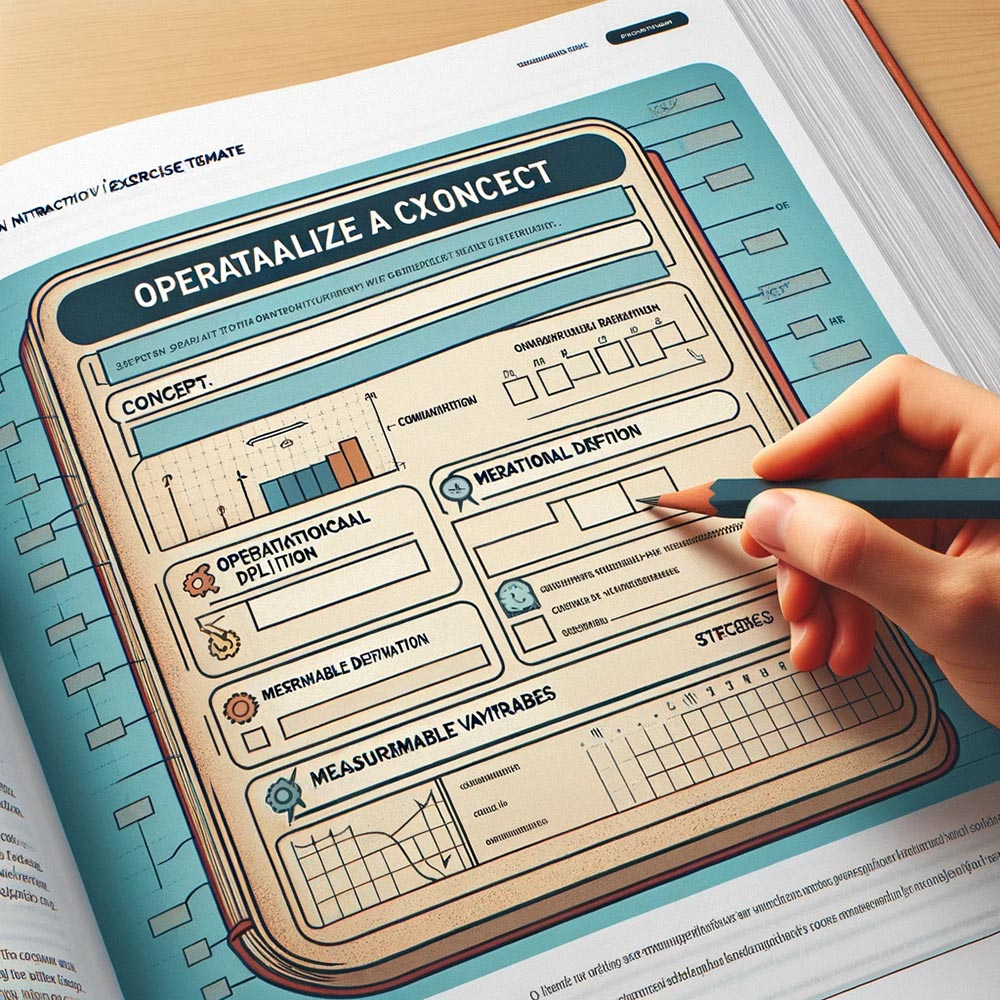
\includegraphics[width=1\textwidth,height=\textheight]{images/fig015.jpg}

*Figure 015. An interactive example or exercise embedded within the textbook. The image could show a blank template for operationalizing a concept, with prompts for students to fill in. For example, the template could ask, ``Concept: \_\textbf{,'' ``Operational Definition: },'' ``Measurable Variables: \_\_\_\_.'' This image would provide a hands-on tool for students to apply what they have learned directly in the textbook.*

By the end of this section, you should have a solid understanding of the importance of conceptual definitions and operationalization in research. You will be equipped to define abstract concepts clearly and determine how to measure them effectively in your studies. This foundational knowledge is essential for conducting rigorous research that produces reliable and valid results, contributing to a deeper understanding of the complex phenomena in mass media.

\subsection{Constructing Hypotheses}\label{constructing-hypotheses}

In the research process, constructing hypotheses is a crucial step that allows you to test specific ideas and draw conclusions based on your data. Hypotheses provide a clear direction for your study and help you determine the relationships between variables. There are three key components involved in constructing hypotheses: the \textbf{null hypothesis (H0)}, the \textbf{alternative hypothesis (H1)}, and the \textbf{research question}. Each plays a distinct role in guiding your research and ensuring that your study is focused and methodologically sound.

The \textbf{null hypothesis (H0)} is a statement that asserts there is no effect or no relationship between the variables being studied. It serves as a baseline or default position that you seek to test against. The null hypothesis is important because it provides a clear point of comparison. For example, if you are studying the impact of media consumption on political attitudes, your null hypothesis might state, ``There is no difference in political attitudes between individuals who consume a high amount of media and those who consume a low amount.'' This statement assumes that media consumption has no effect, and your research will involve testing whether this assumption holds true.

Understanding and formulating a null hypothesis is fundamental to conducting rigorous research. By starting with the assumption that there is no effect, you can objectively test whether your data provides sufficient evidence to reject this hypothesis. This approach ensures that your conclusions are based on empirical evidence rather than preconceived notions.

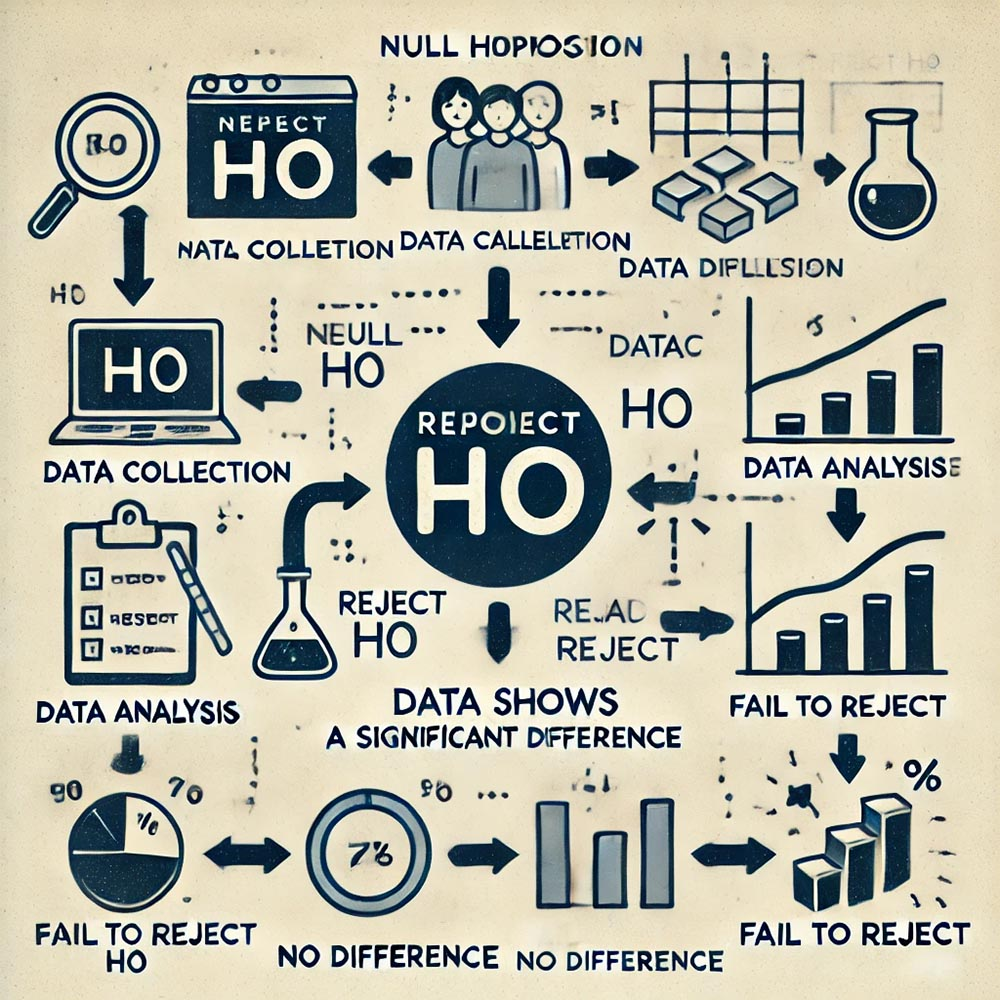
\includegraphics[width=1\textwidth,height=\textheight]{images/fig016.jpg}

\emph{Figure 016. A flowchart showing the process of hypothesis testing, beginning with the null hypothesis (H0) and moving through data collection, analysis, and the decision to either reject or fail to reject the null hypothesis. The chart could include simple examples at each stage, such as ``Data shows no difference'' leading to ``Fail to reject H0'' or ``Data shows a significant difference'' leading to ``Reject H0.'' This visual would help students understand the logical sequence of hypothesis testing.}

In contrast to the null hypothesis, the \textbf{alternative hypothesis (H1)} is a statement that proposes a potential effect or relationship between variables. It directly opposes the null hypothesis and suggests that there is indeed a difference or relationship to be observed. Continuing with the previous example, the alternative hypothesis might state, ``Individuals who consume a high amount of media have different political attitudes than those who consume a low amount.'' This hypothesis suggests that media consumption does influence political attitudes, and your research will aim to determine if this is the case.

The alternative hypothesis is where you articulate the specific effect or relationship you are interested in exploring. It represents the hypothesis you are testing for and is the focus of your research. The goal of your study is to gather enough evidence to support or refute this hypothesis. If the data contradicts the null hypothesis, you may have grounds to accept the alternative hypothesis, indicating that the variables are indeed related.

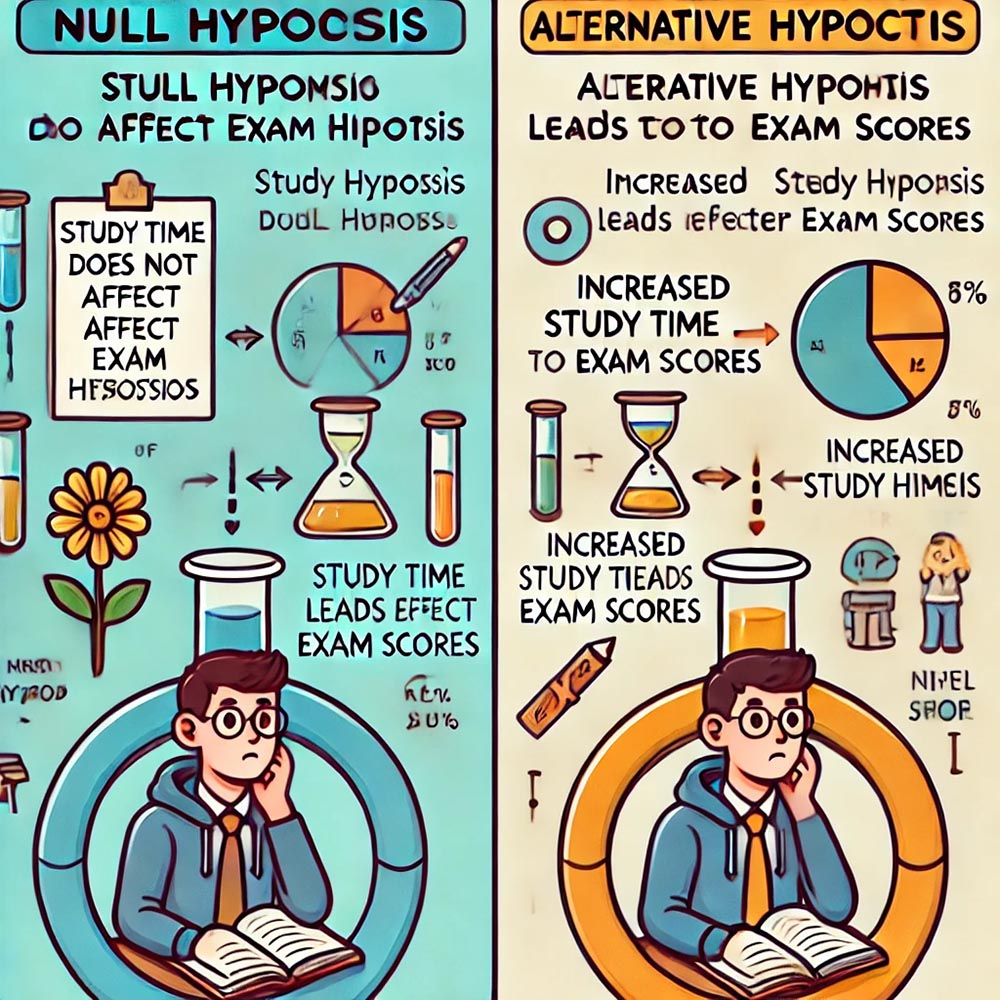
\includegraphics[width=1\textwidth,height=\textheight]{images/fig017.jpg}

\emph{Figure 017. A side-by-side comparison of the null hypothesis and the alternative hypothesis. The image could use a simple example, such as the relationship between study time and exam scores. On one side, the null hypothesis might state, ``Study time does not affect exam scores,'' while the alternative hypothesis might state, ``Increased study time leads to higher exam scores.'' This visual would help students see the contrast between the two types of hypotheses and their roles in research.}

At the heart of hypothesis construction is the \textbf{research question}---the specific query that your study aims to answer. A well-formulated research question is clear, focused, and directly related to the hypotheses you are testing. The research question guides the entire research process, from the design of your study to the analysis of your data. For example, your research question might be, ``How does media consumption influence political attitudes among young adults?'' This question is specific enough to guide your study and broad enough to allow for meaningful analysis.

Crafting a good research question is an essential skill for any researcher. It involves narrowing down broad topics into specific, researchable queries that can be addressed through empirical study. A well-defined research question helps ensure that your study remains focused and that your hypotheses are directly aligned with the goals of your research.

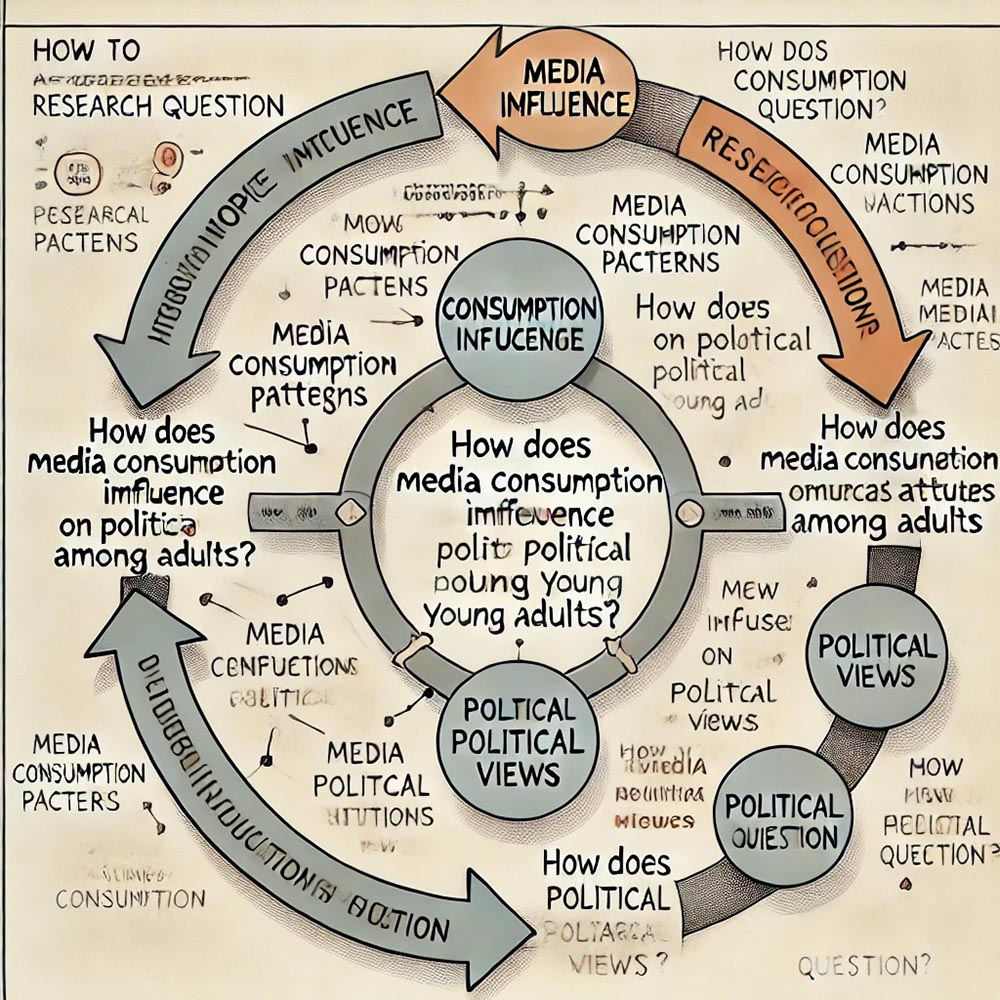
\includegraphics[width=1\textwidth,height=\textheight]{images/fig018.jpg}

\emph{Figure 018. An example of a research question development process. The image could start with a broad topic, such as ``Media Influence,'' and show how it is refined into a specific research question like ``How does media consumption influence political attitudes among young adults?'' Arrows could guide students through the steps of narrowing and focusing the question. This visual would help students understand the process of refining a research topic into a precise and manageable research question.}

In the classroom, we will introduce the concept of the null hypothesis using simple examples that are easy to grasp. For instance, we might start with a hypothesis like ``There is no difference in media consumption between age groups,'' and then explore how this hypothesis can be tested in a research study. You will have the opportunity to write your own null hypotheses for hypothetical studies, helping you to practice formulating clear and testable statements.

We will also discuss the alternative hypothesis, emphasizing how it contrasts with the null hypothesis. By examining real-world research scenarios, you will see how researchers frame their alternative hypotheses to explore specific effects or relationships. In group activities, you will work with your peers to generate both null and alternative hypotheses based on different research questions. This collaborative approach will allow you to apply what you have learned and gain feedback from others.

Finally, we will focus on the research question, discussing the importance of clarity and focus in guiding your study. Through peer feedback sessions, you will refine broad topics into specific research questions that are directly tied to your hypotheses. By the end of this section, you will have the skills to construct well-defined hypotheses and research questions that will guide your studies and contribute to meaningful and impactful research.

\section{Measurement and Variables}\label{measurement-and-variables}

\subsection{Levels of Measurement}\label{levels-of-measurement}

Understanding the different levels of measurement is fundamental to conducting effective research. The level of measurement of your data determines the types of statistical analyses you can perform and how you can interpret your results. There are four primary levels of measurement: nominal, ordinal, interval, and ratio. Each level provides a different way of categorizing and quantifying data, and recognizing these distinctions will enhance your ability to design studies and analyze data accurately.

The \textbf{nominal level} of measurement involves classifying data into distinct categories that do not have a specific order. At this level, data points are simply grouped based on shared characteristics, and these categories are mutually exclusive---each data point fits into one and only one category. For example, in media studies, you might categorize types of media content, such as TV shows, into genres like drama, comedy, and documentary. Each genre represents a nominal category, and while these categories help you organize the data, they do not imply any ranking or order among them.

Nominal data is particularly useful when your goal is to count the frequency of occurrences in each category or when you need to distinguish between different types of entities. However, because nominal data lacks an inherent order, you cannot perform mathematical operations like addition or subtraction on it. Understanding the limitations and appropriate uses of nominal data is crucial for ensuring the accuracy of your analyses.

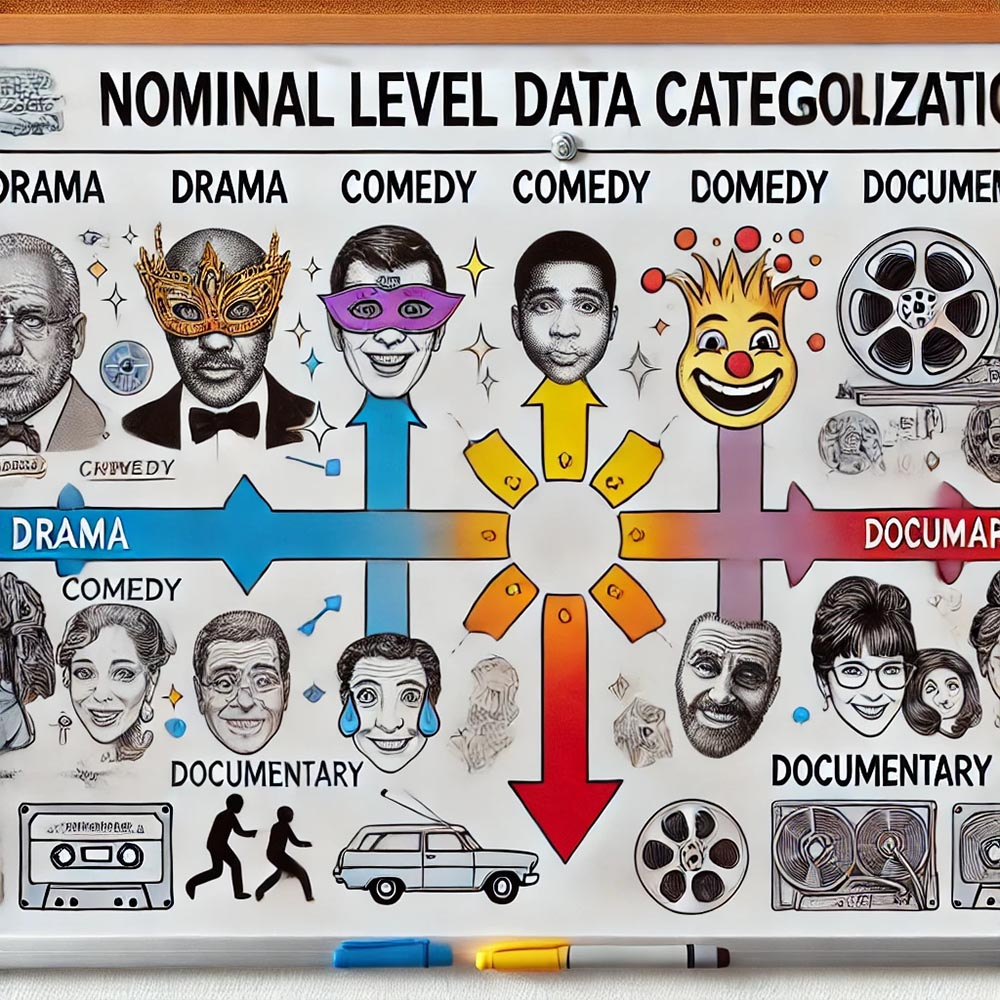
\includegraphics[width=1\textwidth,height=\textheight]{images/fig019.jpg}

\emph{Figure 019. A chart illustrating nominal level data categorization. The image could display different TV show genres (e.g., drama, comedy, documentary) with visual icons representing each genre. Arrows could show how individual TV shows are categorized into these genres. This visual would help students grasp the concept of nominal categorization and its application in media studies.}

The \textbf{ordinal level} of measurement takes categorization a step further by introducing a meaningful order among the categories. At this level, data is ranked or ordered in a way that reflects a relative position or degree, but the intervals between the ranks are not necessarily consistent. For example, consider a survey that asks participants to rank their favorite media channels from most to least preferred. The resulting data shows the order of preference, but it does not indicate how much more one channel is preferred over another.

Ordinal data is often used in research to assess relative standings or preferences. However, because the distances between the ranks are not equal or known, you cannot assume that the difference between two ranks is the same as the difference between two other ranks. This limitation affects the types of statistical analyses that can be performed, making it important to choose the right level of measurement for your research question.

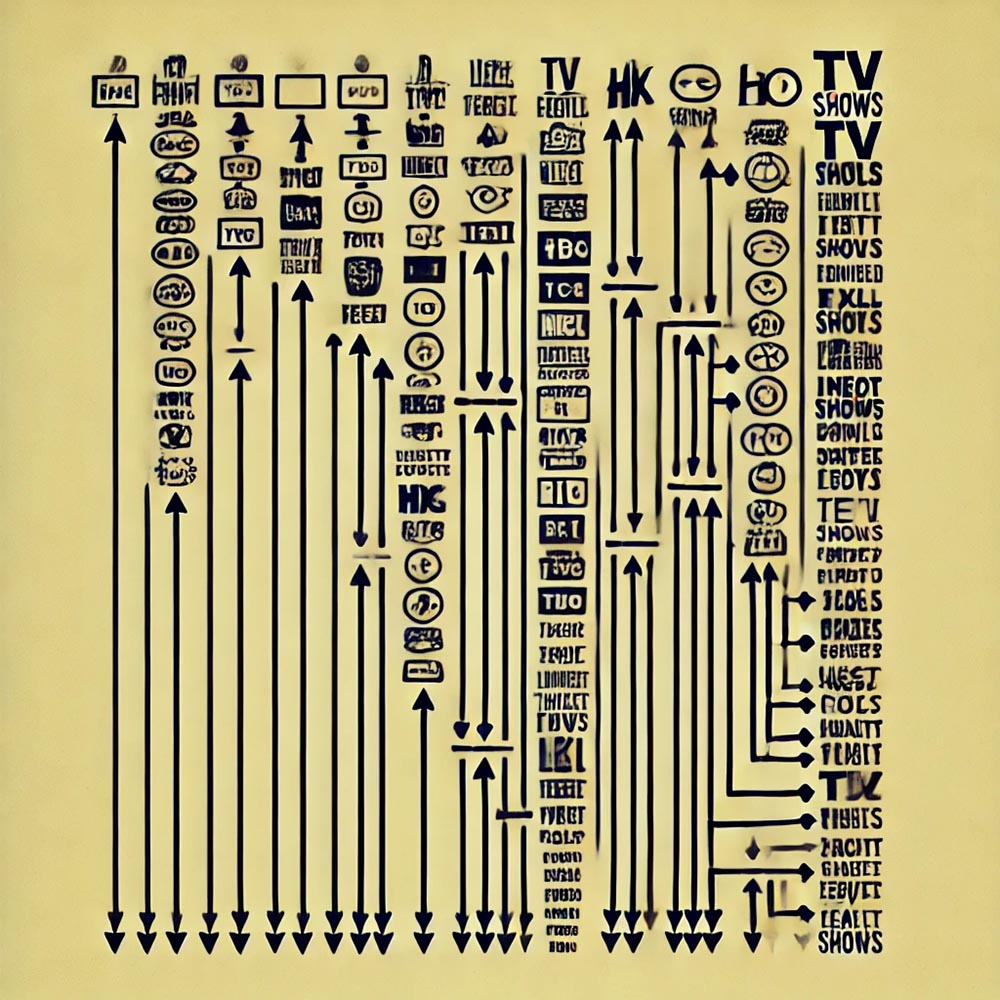
\includegraphics[width=1\textwidth,height=\textheight]{images/fig020.jpg}

\emph{Figure 020. An example of ordinal data representation. The image could show a ranking of favorite TV shows, with each show placed in a specific order but without equal spacing between the ranks. A visual representation of the rankings, such as a list with arrows indicating the order, would help students understand how ordinal data is structured and interpreted.}

Moving beyond ordinal data, the \textbf{interval level} of measurement involves numerical data where the intervals between values are consistent, but there is no true zero point. This means that while you can measure the distance between data points, the lack of a true zero means that you cannot make meaningful statements about the absolute quantity or ratio of the data. A common example of interval data in media research is the Likert scale, often used in surveys to assess attitudes or opinions. On a Likert scale, participants might rate their agreement with a statement on a scale from 1 to 5, where each interval between numbers is equal.

Interval data allows for a wider range of statistical analyses than nominal or ordinal data, as you can calculate means and standard deviations. However, because interval data lacks a true zero point, certain operations, like calculating ratios, are not meaningful. For instance, saying that a score of 4 on a Likert scale is ``twice as positive'' as a score of 2 is not valid, as the scale does not represent an absolute quantity.

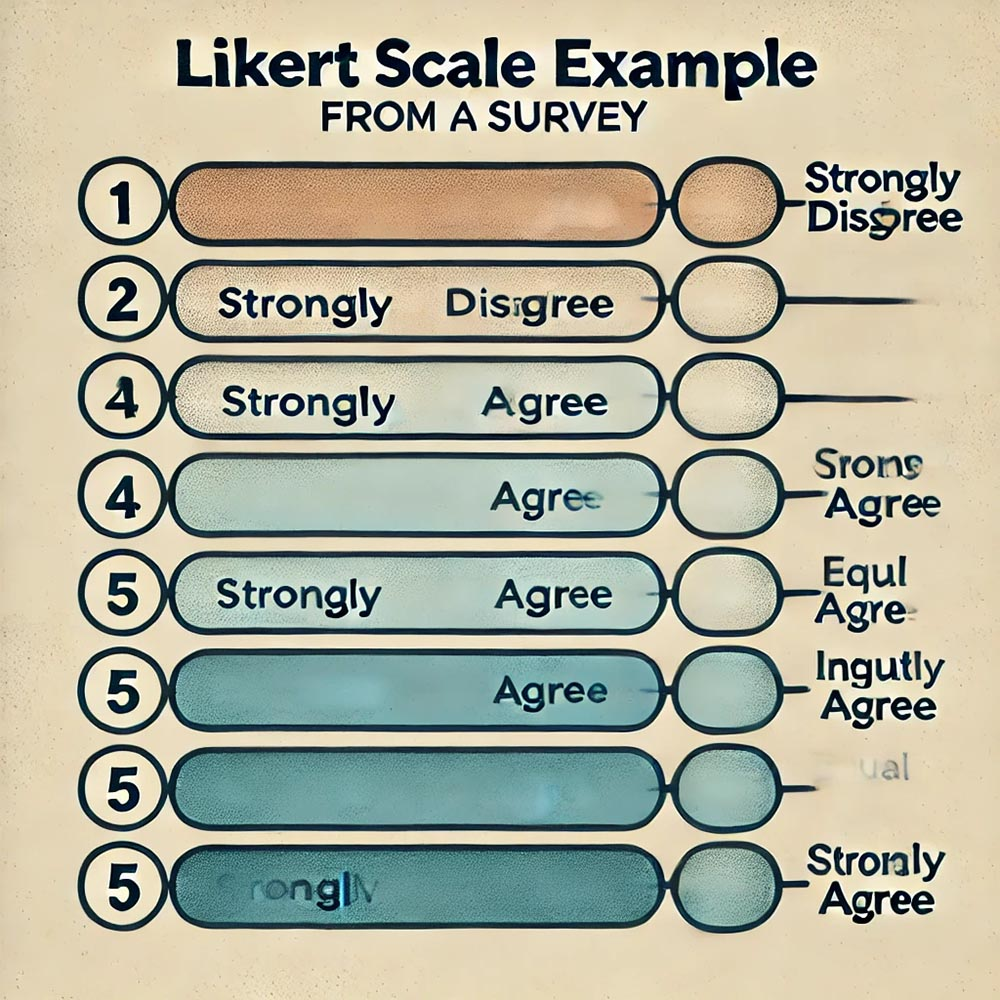
\includegraphics[width=1\textwidth,height=\textheight]{images/fig021.jpg}

\emph{Figure 021. A Likert scale example from a survey, showing a range from 1 (Strongly Disagree) to 5 (Strongly Agree). Each point on the scale should be evenly spaced to emphasize the equal intervals between them. This visual would clarify how interval data is structured and why the equal spacing is important for analysis.}

Finally, the \textbf{ratio level} of measurement is the most informative level, as it includes all the properties of the interval level but also has a true zero point. This means that not only can you measure the distance between data points, but you can also make meaningful statements about the absolute quantities and ratios of the data. An example of ratio data in media research could be the number of hours individuals spend watching TV per week. Since there is a true zero point (zero hours means no TV watched), you can say that someone who watches 10 hours of TV per week watches twice as much as someone who watches 5 hours.

Ratio data provides the greatest flexibility for statistical analysis, allowing you to use all mathematical operations, including calculating means, variances, and ratios. Understanding and correctly identifying ratio data is crucial for conducting accurate and meaningful research, as it allows for the most precise and comprehensive analysis.

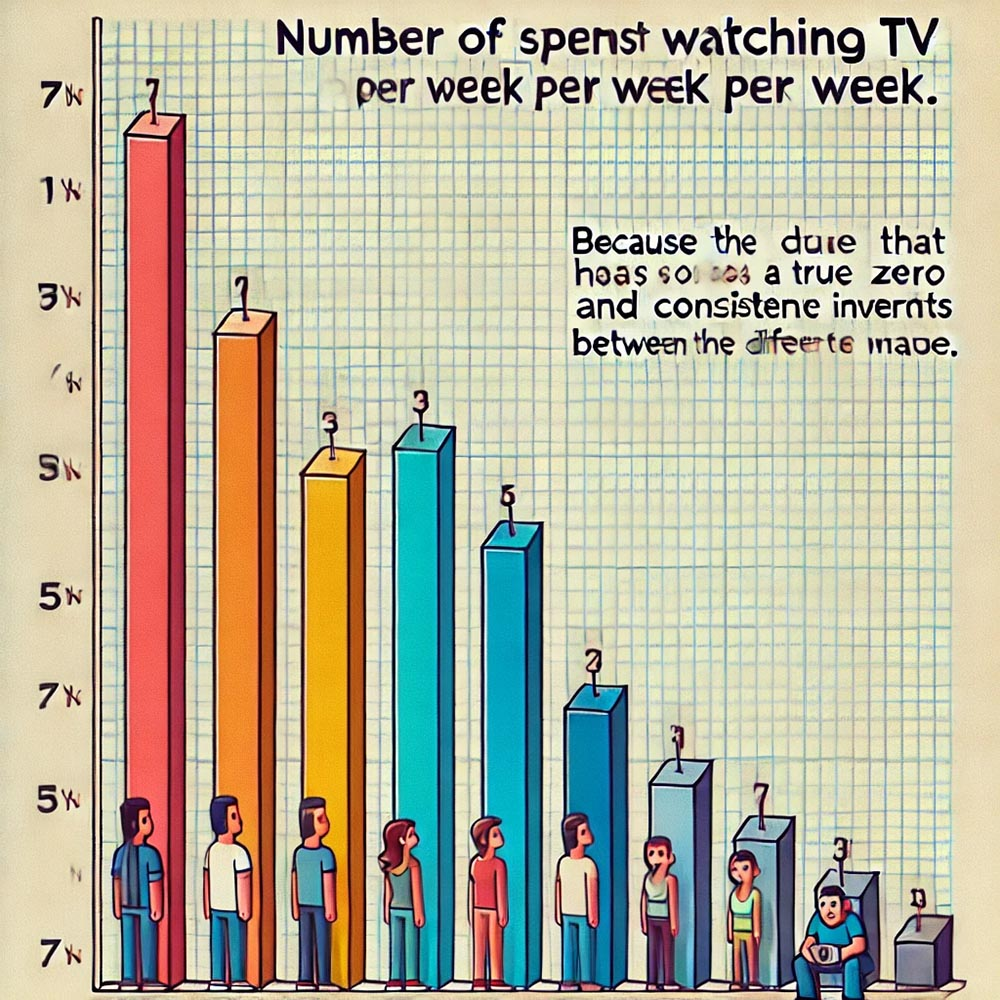
\includegraphics[width=1\textwidth,height=\textheight]{images/fig022.jpg}

\emph{Figure 022. A bar graph showing the number of hours spent watching TV per week by different individuals. The graph could highlight that the data has a true zero point and uses consistent intervals, showing how this allows for meaningful comparisons between different values. This visual would help students understand the concept of ratio data and its application in research.}

In the classroom, we will explore these levels of measurement through interactive exercises. For instance, you might classify different types of media content into nominal categories or arrange survey data in an ordinal manner to see how the order affects interpretation. Additionally, we will engage in activities where you design surveys using interval-level measures and identify ratio-level variables in research articles. These hands-on experiences will reinforce your understanding of the different levels of measurement and their implications for data analysis.

By mastering these concepts, you will be equipped to choose the appropriate level of measurement for your research questions and apply the correct statistical techniques to analyze your data. This foundational knowledge is essential for conducting rigorous and reliable research in the field of mass media.

\subsection{Identifying Independent and Dependent Variables}\label{identifying-independent-and-dependent-variables}

In research, understanding the roles of independent and dependent variables is essential for designing experiments and interpreting results. These variables help researchers establish cause-and-effect relationships by manipulating one factor and observing the impact on another. Grasping these concepts will enable you to clearly define your research questions and hypotheses and to structure your studies in a way that yields meaningful data.

The \textbf{independent variable (IV)} is the variable that the researcher manipulates or categorizes to observe its effect on another variable. It is considered the ``cause'' in a cause-and-effect relationship. For instance, in a study exploring the impact of different types of media content on audience engagement, the type of media content (e.g., news, entertainment, educational) would be the independent variable. The researcher changes or selects different categories of media content to see how these variations influence the outcome, which is the dependent variable.

To help you better understand independent variables, consider an experiment where you want to study how different advertising formats affect consumer behavior. The independent variable could be the format of the advertisement---such as a video, a banner ad, or a social media post. By manipulating the format, you can observe how these changes influence consumer behavior, such as click-through rates or purchasing decisions.

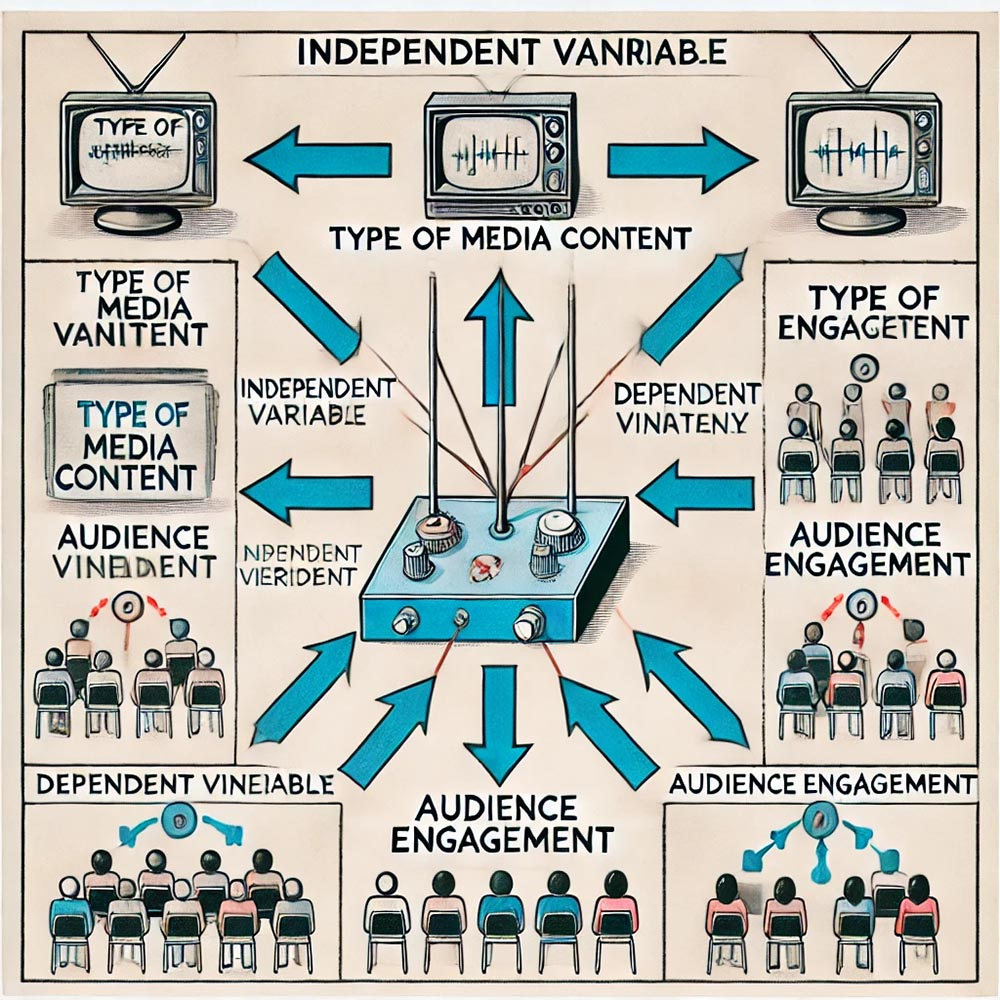
\includegraphics[width=1\textwidth,height=\textheight]{images/fig023.jpg}

\emph{Figure 023. A diagram showing an experiment where the independent variable (e.g., ``Type of Media Content'') is manipulated to observe its effect on the dependent variable (e.g., ``Audience Engagement''). The diagram could use arrows to indicate the direction of influence from the independent variable to the dependent variable. This visual would help students see the relationship between these variables in a research context.}

On the other hand, the \textbf{dependent variable (DV)} is the variable that is measured and is expected to be influenced by changes in the independent variable. It is considered the ``effect'' in the cause-and-effect relationship. Continuing with the previous example of media content, the dependent variable might be audience engagement, which could be measured in various ways, such as the number of comments, likes, shares, or time spent viewing the content. The key here is that the dependent variable is what you observe and record as data to determine if and how it changes in response to the independent variable.

To illustrate the role of dependent variables, imagine a study where you are investigating how different headlines affect readers' perceptions of news credibility. The dependent variable could be the credibility score that readers assign to each article after reading it. By measuring this score, you can assess whether changes in the headline (the independent variable) have an impact on readers' perceptions of credibility (the dependent variable).

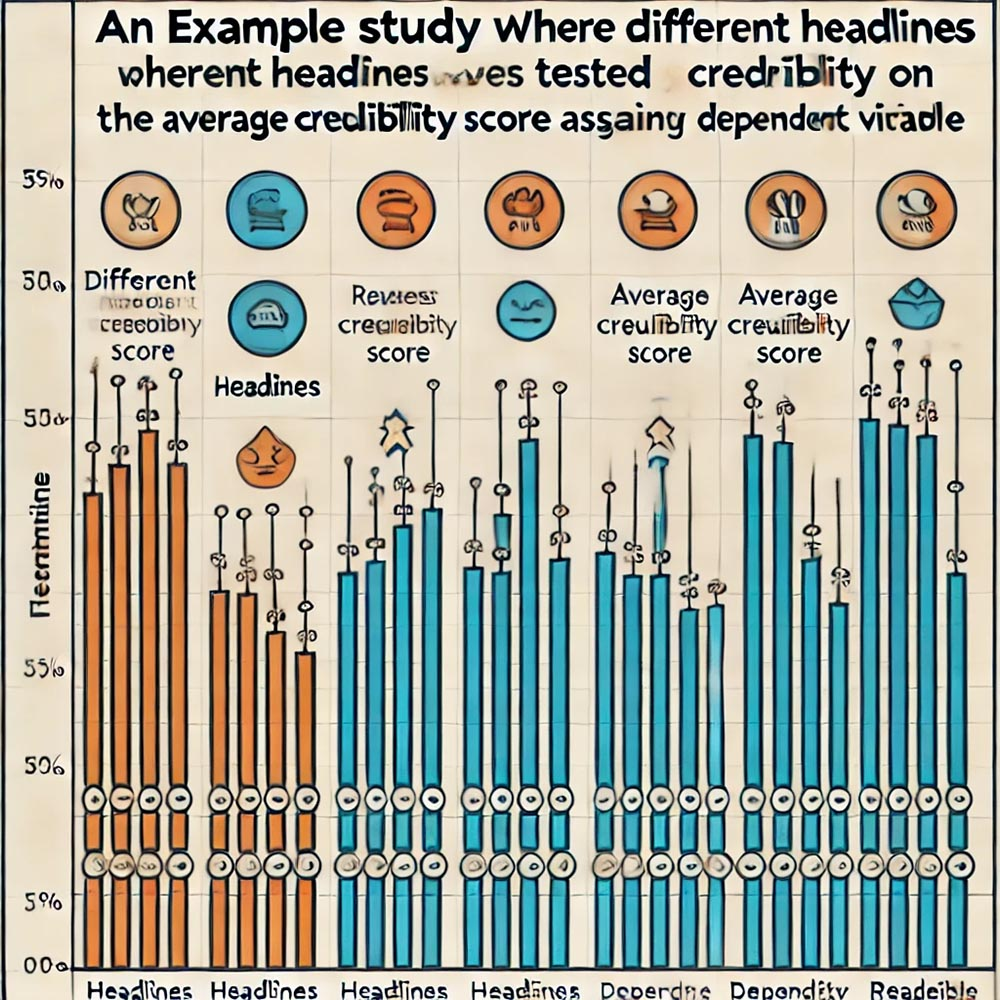
\includegraphics[width=1\textwidth,height=\textheight]{images/fig024.jpg}

\emph{Figure 024. A chart displaying an example study where different headlines (independent variable) are tested against readers' credibility scores (dependent variable). The chart could show varying scores based on different headlines, visually representing the effect of the independent variable on the dependent variable. This image would help students understand how changes in the independent variable can influence the dependent variable.}

In the classroom, we will explore these concepts by examining case studies where the independent and dependent variables are clearly identified. For example, we might look at a research study that examines the effect of social media usage on academic performance. In this case, social media usage would be the independent variable, while academic performance, measured through grades or test scores, would be the dependent variable. By analyzing these case studies, you will learn how to distinguish between the variables and understand their roles in research.

To reinforce your understanding, you will also engage in activities where you map out research scenarios and clearly define the independent and dependent variables. For instance, you might be tasked with designing a study to investigate how different levels of advertising exposure (independent variable) influence brand recall (dependent variable). By defining these variables, you will gain practical experience in structuring research questions and experiments.

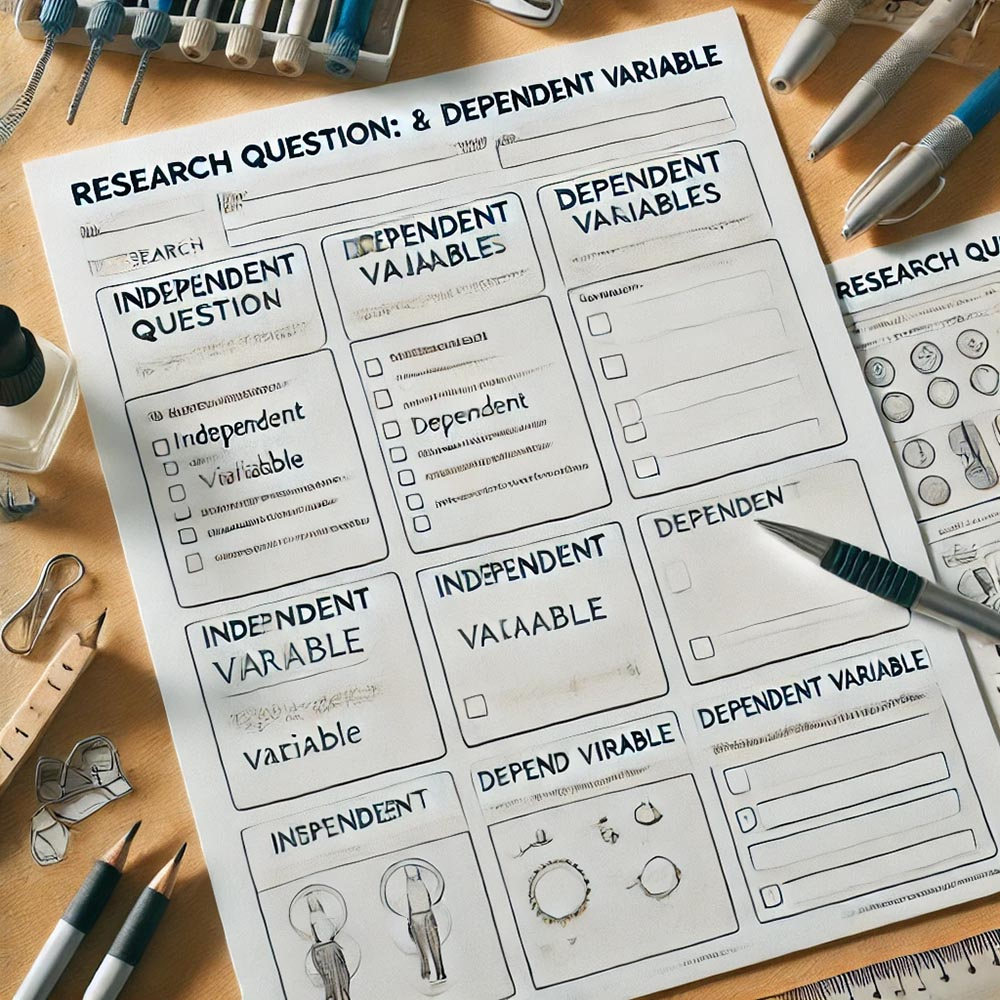
\includegraphics[width=1\textwidth,height=\textheight]{images/fig025.jpg}

\emph{Figure 025. A worksheet or template where students can practice identifying and defining independent and dependent variables in various research scenarios. The worksheet could include prompts like ``Research Question:'', ``Independent Variable: \textbf{'', and ''Dependent Variable: }\_''. This interactive element would provide a hands-on tool for students to apply what they have learned.}

By the end of this section, you should be confident in your ability to identify independent and dependent variables in a wide range of research contexts. This foundational knowledge will be crucial as you move forward in your studies, allowing you to design experiments that effectively test your hypotheses and contribute to the broader understanding of mass media effects. Understanding these variables will also enable you to critically evaluate existing research, helping you discern the validity of the studies you encounter in academic literature.

\subsection{Issues in Measurement}\label{issues-in-measurement}

When conducting research, particularly in the social sciences and media studies, accurate and consistent measurement is crucial. However, various challenges can arise in the measurement process, leading to potential errors and inaccuracies. Understanding these issues, such as \textbf{measurement error}, \textbf{validity}, and \textbf{reliability}, is essential for ensuring that your research findings are both accurate and meaningful.

\textbf{Measurement error} refers to the difference between the observed value and the true value of what is being measured. It can occur for a variety of reasons, and even small errors can significantly impact the validity of your research results. Common sources of measurement error include respondent misunderstanding, data entry mistakes, and inconsistencies in how data is collected. For instance, if participants in a survey misinterpret a question, their responses may not accurately reflect their true attitudes or behaviors, leading to measurement error. Similarly, if data is entered incorrectly into a database, the resulting analysis could be skewed.

Understanding and identifying sources of measurement error is key to minimizing its impact on your research. For example, consider a study measuring the effectiveness of a new media literacy program. If participants misunderstand a survey question about their media consumption habits, the resulting data might inaccurately represent their actual media use. This could lead to incorrect conclusions about the program's effectiveness.

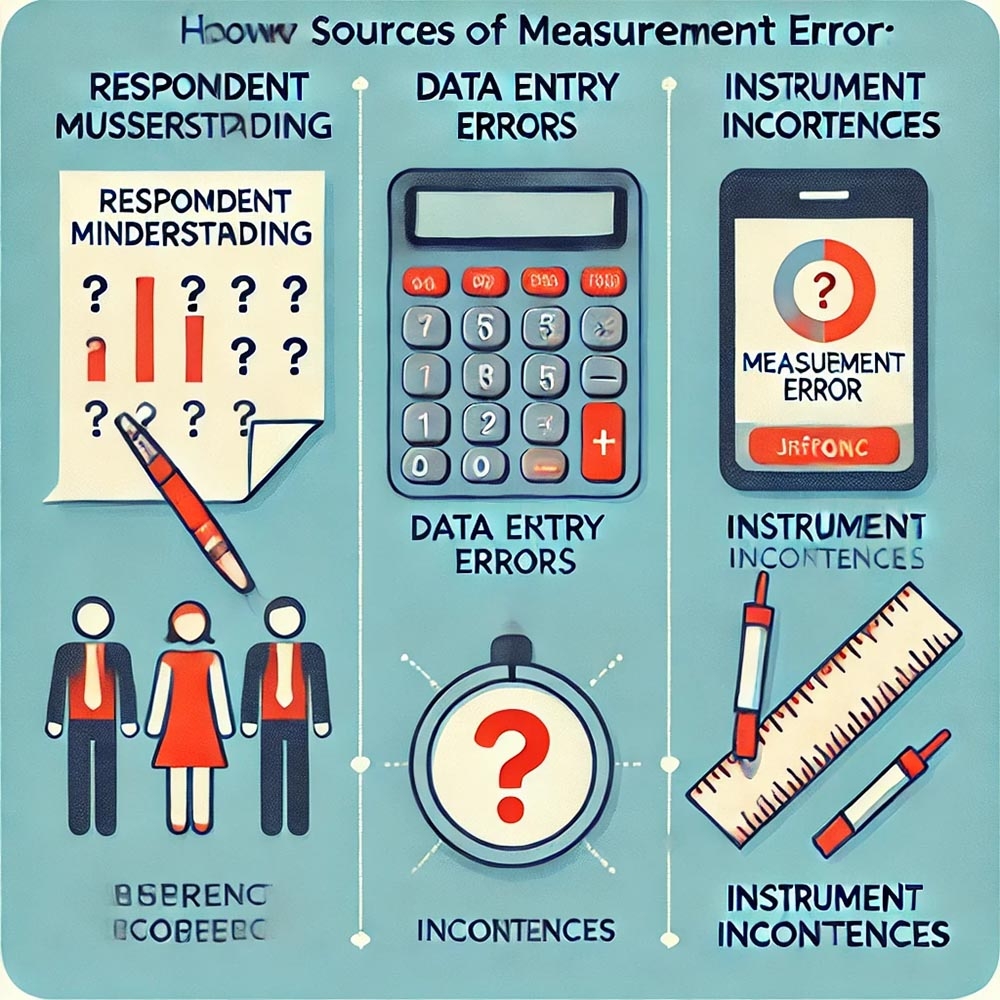
\includegraphics[width=1\textwidth,height=\textheight]{images/fig026.jpg}

\emph{Figure 026. An infographic showing different sources of measurement error. The image could include icons representing respondent misunderstanding (e.g., a question mark over a survey response), data entry errors (e.g., a keyboard with a typo), and instrument inconsistencies (e.g., a broken ruler). This visual would help students recognize various types of measurement error and their potential impact on research outcomes.}

To help you grasp the concept of measurement error, we will discuss practical examples of how such errors can affect research outcomes. We will explore case studies where measurement error led to misleading results and analyze how these errors could have been avoided. Additionally, we will conduct a class exercise where you will be asked to identify potential sources of measurement error in a given study. This hands-on activity will help you develop the skills to recognize and address measurement error in your own research.

\textbf{Validity} is another critical issue in measurement. It refers to the extent to which a measurement tool accurately measures what it is intended to measure. If a tool lacks validity, the data it produces may not truly reflect the concept under study, leading to faulty conclusions. There are different types of validity, but one of the most important in social sciences research is \textbf{construct validity}. Construct validity ensures that the test or measurement tool effectively measures the concept it's intended to measure.

For example, in media studies, psychological scales are often used to measure abstract concepts like media literacy or audience engagement. To assess the construct validity of such a scale, you would need to determine whether the scale truly captures the essence of the concept it aims to measure. If the scale includes irrelevant items or fails to address key aspects of the concept, its validity would be compromised.

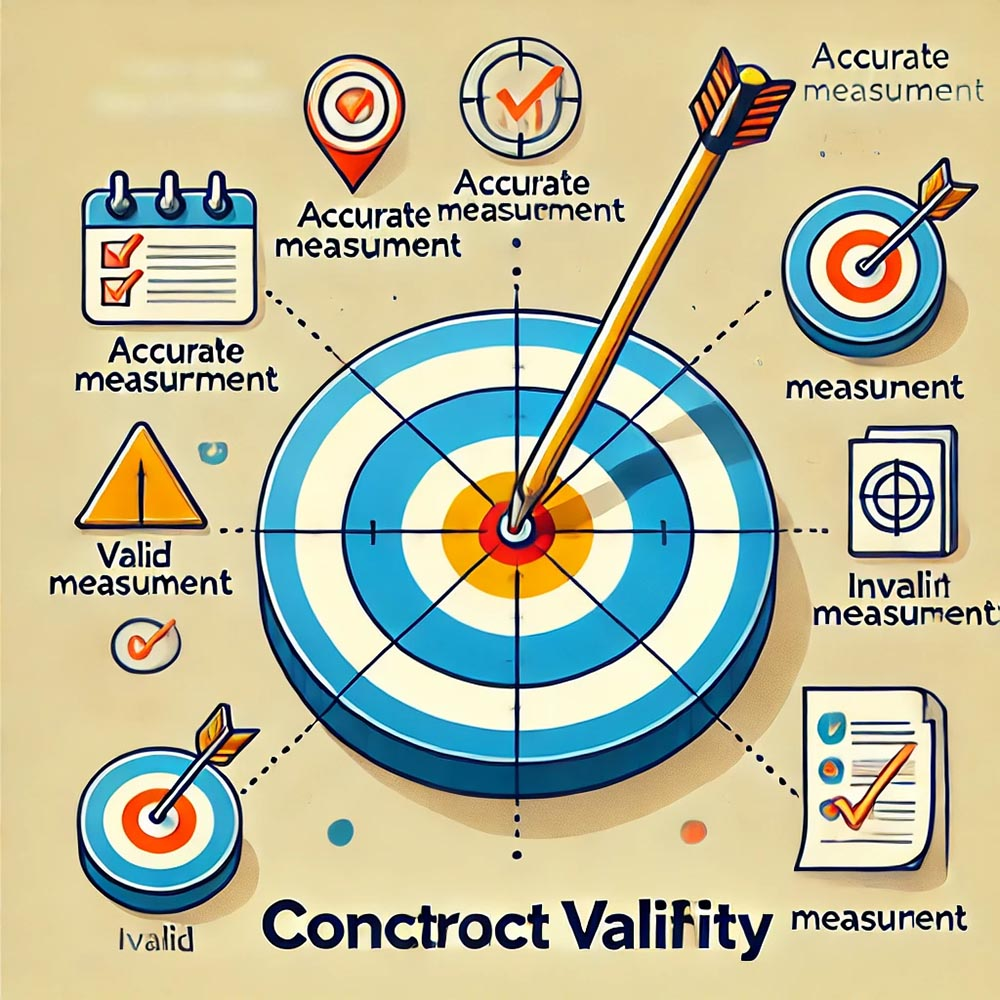
\includegraphics[width=1\textwidth,height=\textheight]{images/fig027.jpg}

\emph{Figure 027. A diagram illustrating the concept of construct validity. The image could show a target with an arrow hitting the center, labeled ``Accurate Measurement,'' to symbolize valid measurement. Surrounding the target, there could be examples of both valid and invalid measures, helping students visualize the importance of hitting the ``target'' with their measurement tools.}

In our discussions, we will use examples from existing psychological scales used in media studies to explore how validity is assessed. You will have the opportunity to evaluate the validity of research tools by considering whether they effectively measure the intended concepts. This exercise will deepen your understanding of how to ensure that your own measurement tools are valid, leading to more accurate and credible research findings.

Finally, we must consider \textbf{reliability}, which refers to the consistency of a measurement tool in producing the same results under the same conditions. If a tool is reliable, it should yield similar results each time it is used in the same situation. For example, a standardized test that consistently produces the same scores for a student across different administrations would be considered reliable.

Reliability is crucial because it ensures that your measurements are stable and repeatable. Without reliability, even valid measurements can be rendered meaningless, as inconsistent results can obscure the true relationships between variables. For instance, if a survey instrument designed to measure audience engagement produces wildly different results each time it is administered, it would be difficult to draw any reliable conclusions about audience behavior.

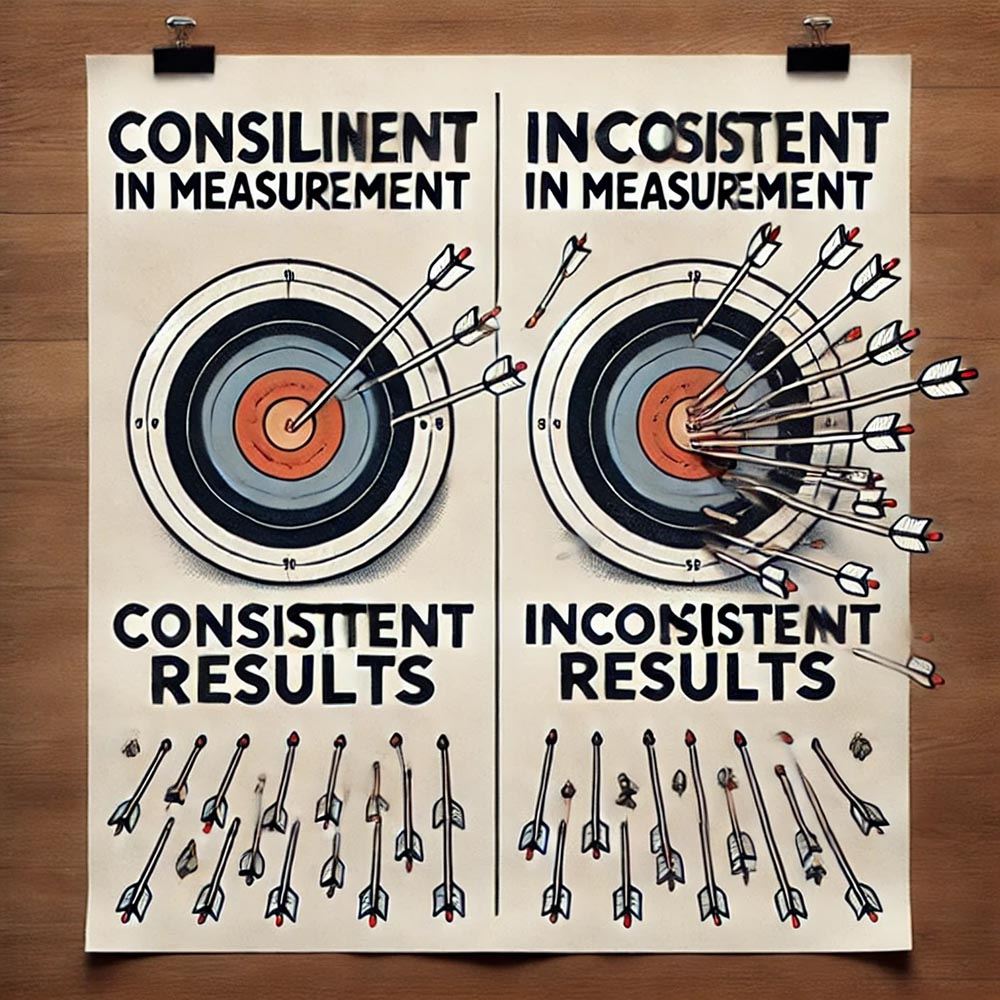
\includegraphics[width=1\textwidth,height=\textheight]{images/fig028.jpg}

\emph{Figure 028. A visual representation of reliability in measurement. The image could depict multiple arrows consistently hitting the same spot on a target, labeled ``Consistent Results.'' Alongside this, another target could show arrows scattered all over, labeled ``Inconsistent Results,'' to illustrate unreliable measurement. This visual would help students understand the concept of reliability and its importance in research.}

To reinforce the concept of reliability, we will engage in an exercise where you will test the reliability of a simple survey instrument over repeated trials. By analyzing the consistency of the results, you will gain a practical understanding of how to assess and improve the reliability of your own measurement tools.

Throughout this section, you will learn to recognize and address the key issues in measurement that can impact the accuracy and credibility of your research. By understanding and applying the concepts of measurement error, validity, and reliability, you will be better equipped to design studies that produce meaningful and trustworthy results.

\chapter{Designing Quantitative Research}\label{designing-quantitative-research}

\section{Research Design}\label{research-design}

\subsection{Experimental Designs}\label{experimental-designs}

Experimental designs are a powerful tool in research, allowing you to test hypotheses and establish causal relationships between variables. In mass media research, these designs are particularly useful for exploring how different types of media content affect audience behavior and perception. There are several types of experimental designs, each with its own strengths and challenges. Understanding how to properly implement these designs is crucial for conducting valid and reliable research.

One of the most commonly used experimental designs is the \textbf{between-subjects design}. In a between-subjects design, different participants are assigned to different groups, and each group is exposed to a different level of the independent variable. This design allows you to compare the effects of various conditions on different groups of participants. For example, you might have one group of participants watch a news broadcast with a positive tone, while another group watches the same broadcast with a negative tone. By measuring differences in audience perception between these two groups, you can determine the impact of the tone of the broadcast on how the news is received.

This approach is particularly effective when you want to ensure that the effects you are observing are due to the independent variable rather than other factors. Because each group only experiences one condition, there is less risk of participants becoming biased or fatigued by multiple exposures. However, between-subjects designs also require careful consideration of group equivalence, ensuring that any differences between groups are due to the experimental manipulation and not pre-existing differences among participants.

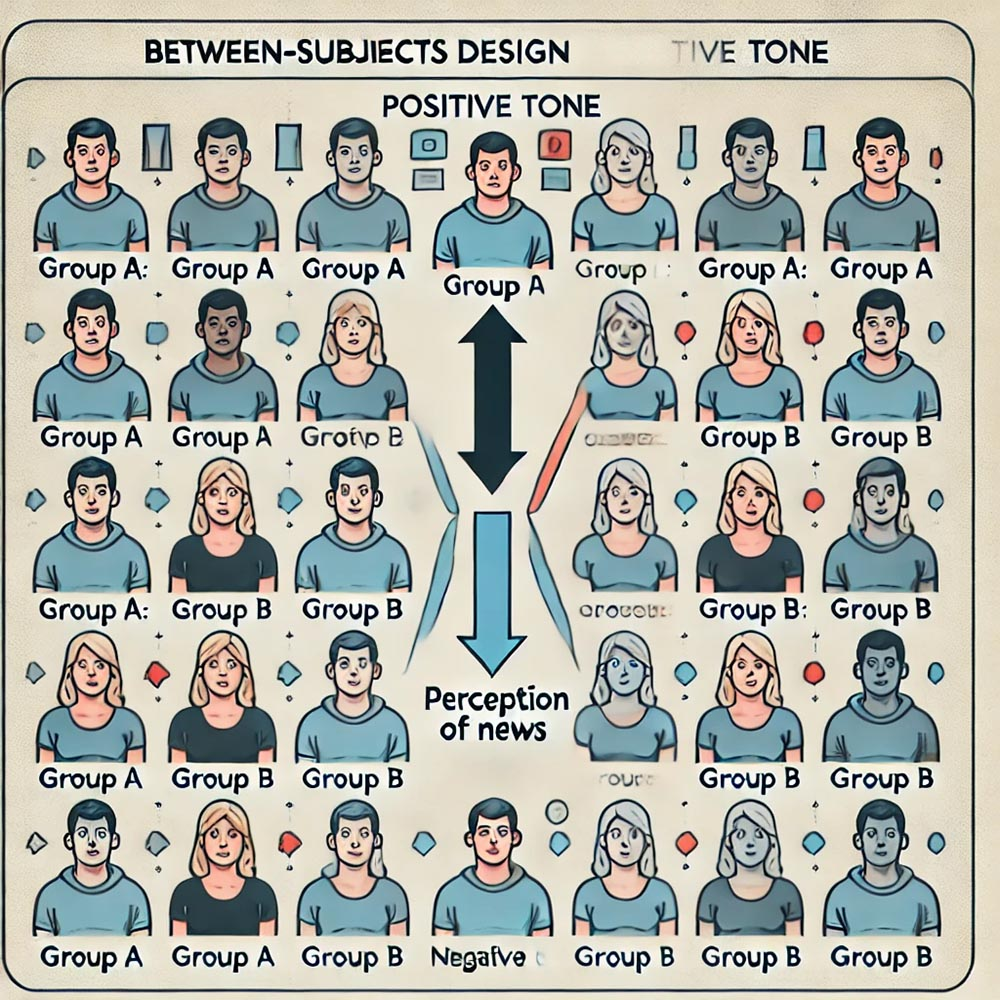
\includegraphics[width=1\textwidth,height=\textheight]{images/fig029.jpg}

\emph{Figure 029. A diagram illustrating a between-subjects design. The image could show two groups of participants, with one group labeled ``Group A: Positive Tone'' and the other ``Group B: Negative Tone.'' Arrows could point from each group to a measurement outcome, such as ``Perception of News.'' This visual would help students understand how different conditions are applied to different groups in a between-subjects design.}

In contrast to the between-subjects design, a \textbf{within-subjects design} involves exposing the same participants to all levels of the independent variable. This design allows for direct comparison within the same group, making it easier to observe how changes in the independent variable affect participants. For instance, you might have participants first watch a positive news broadcast and then a negative one, measuring their reactions after each. Because the same individuals experience both conditions, you can more accurately assess the impact of the variable by comparing their responses.

Within-subjects designs are particularly useful when you want to control for individual differences, as each participant serves as their own control. However, this design can also introduce potential issues like order effects, where the sequence in which conditions are presented affects the results. For example, participants might become more critical or fatigued after watching multiple broadcasts, which could influence their responses. To mitigate these effects, researchers often use techniques such as counterbalancing, where the order of conditions is varied across participants.

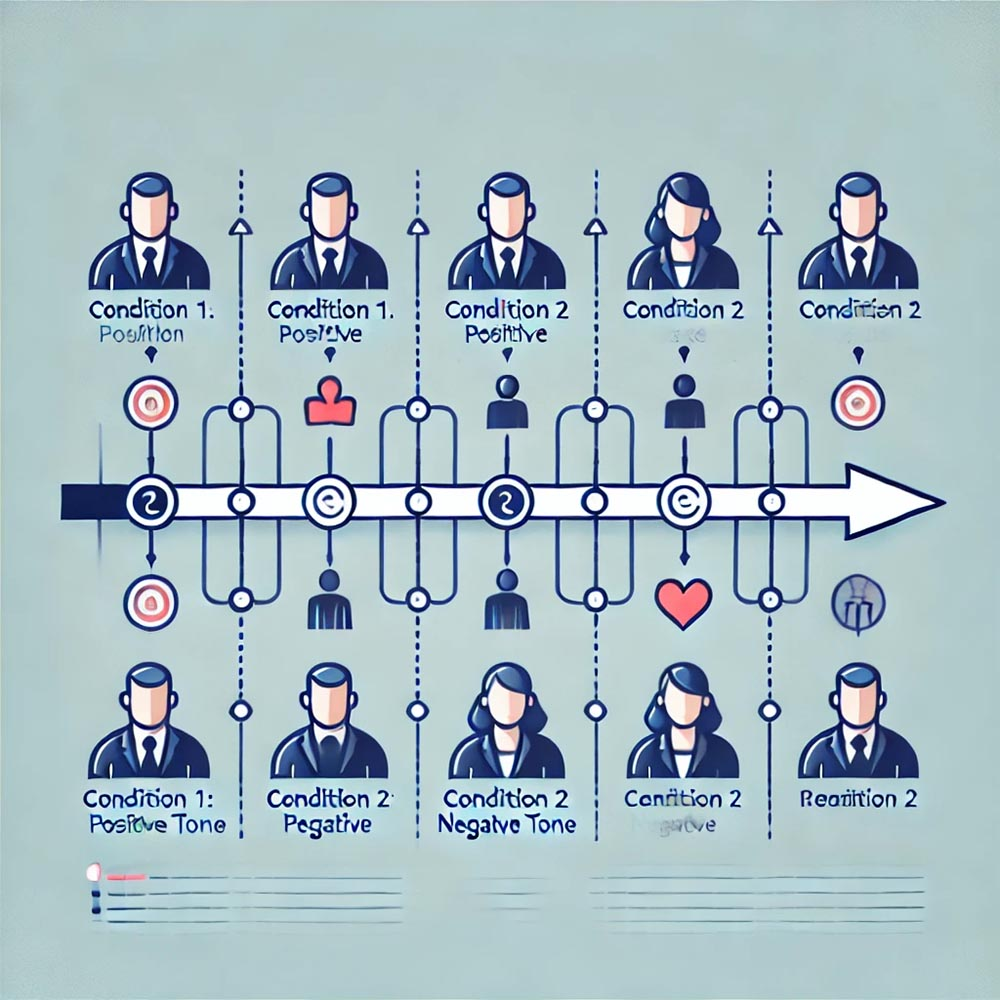
\includegraphics[width=1\textwidth,height=\textheight]{images/fig030.jpg}

\emph{Figure 030. A timeline showing a within-subjects design. The image could depict a single group of participants experiencing two conditions in sequence, labeled ``Condition 1: Positive Tone'' followed by ``Condition 2: Negative Tone.'' Arrows could point to their measured reactions after each condition. This visual would help students see how within-subjects designs allow for direct comparison within the same group.}

A crucial component of any experimental design is the inclusion of a \textbf{control group}. The control group is composed of participants who do not receive the experimental treatment and serve as a baseline for comparison. In a study on media influence, for example, the control group might be exposed to neutral media content, while the experimental groups receive content with a specific bias. By comparing the responses of the control group to those of the experimental groups, you can determine whether the independent variable (in this case, the media bias) has a significant effect.

Control groups are essential for isolating the effect of the independent variable and ruling out alternative explanations for your findings. Without a control group, it would be difficult to determine whether observed changes are due to the manipulation or other factors. For instance, if both the experimental and control groups show similar changes in perception, this might suggest that factors other than the media content are at play.

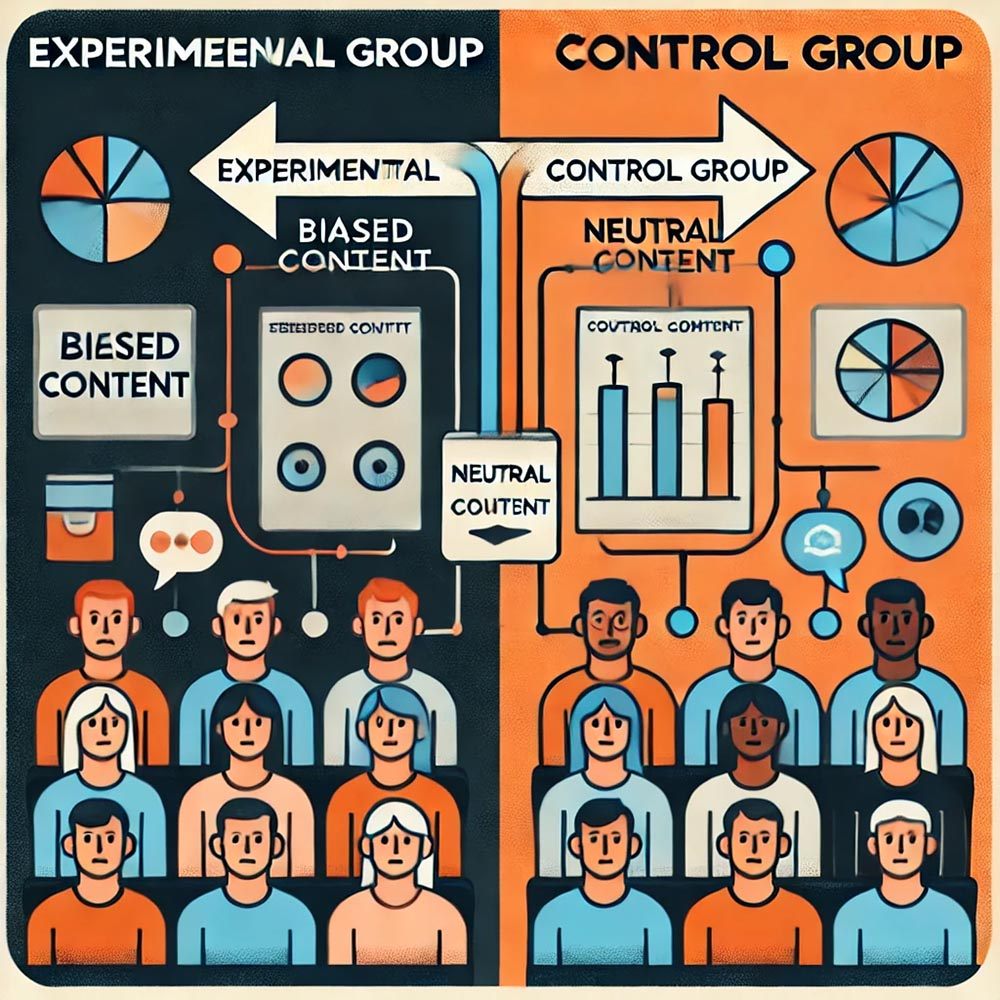
\includegraphics[width=1\textwidth,height=\textheight]{images/fig031.jpg}

\emph{Figure 031. A side-by-side comparison of an experimental group and a control group. The image could show one group labeled ``Experimental Group: Biased Content'' and another labeled ``Control Group: Neutral Content,'' with arrows leading to different outcome measures. This visual would help students understand the role of a control group in providing a baseline for comparison in experimental research.}

In the classroom, we will explore these concepts through case studies and practical exercises. We will begin by examining examples from mass media research where between-subjects designs have been applied, helping you understand how different conditions can be tested across groups. We will also conduct a classroom experiment where you are split into groups and exposed to different media stimuli. Afterward, we will discuss the results, focusing on how the different designs affected the outcomes.

To further illustrate within-subjects designs, we will use simple examples, such as testing the effect of different headlines on the same group's perception of a news story. You will be assigned a project where you design your own within-subjects experiment, identifying potential issues like order effects and discussing strategies to counter them.

Finally, we will delve into the importance of control groups by discussing real-world examples and having you design an experiment where you implement a control group. You will also discuss why control groups are necessary and how they contribute to the validity of your findings.

By mastering these experimental designs, you will be better equipped to conduct rigorous and reliable research, allowing you to draw meaningful conclusions about the effects of media on audiences. This foundational knowledge is essential for any researcher in mass communications and will serve you well in your future studies and professional work.

\subsection{Non-experimental Designs}\label{non-experimental-designs}

In research, not all studies require or even allow for experimental manipulation. In many cases, researchers must rely on non-experimental designs to observe and analyze data as it naturally occurs. Two common non-experimental designs used in mass media research are cross-sectional designs and longitudinal designs. Each of these approaches offers distinct advantages and challenges, and understanding their applications is essential for conducting meaningful research when experiments are not feasible.

\textbf{Cross-sectional designs} are one of the most frequently used non-experimental approaches. This design involves observing a specific population at a single point in time. By collecting data from participants all at once, researchers can identify patterns, trends, and relationships between variables. For example, you might conduct a survey to assess the public's opinion on the influence of social media at a particular moment. The data collected in a cross-sectional study can provide a snapshot of the current state of a population's views, behaviors, or characteristics.

One of the primary advantages of cross-sectional designs is their efficiency. Because data is collected at a single point in time, these studies can be completed relatively quickly and are often less expensive than other research designs. They are particularly useful for descriptive studies that aim to understand the prevalence or distribution of a phenomenon within a population.

However, while cross-sectional designs are excellent for identifying relationships between variables, they have significant limitations when it comes to inferring causality. Since the data is collected at only one point in time, it is difficult to determine the direction of relationships between variables or to establish cause-and-effect relationships. For instance, if you find that individuals who spend more time on social media have higher levels of anxiety, a cross-sectional study cannot tell you whether social media use causes anxiety, whether anxiety leads to increased social media use, or whether another factor influences both.

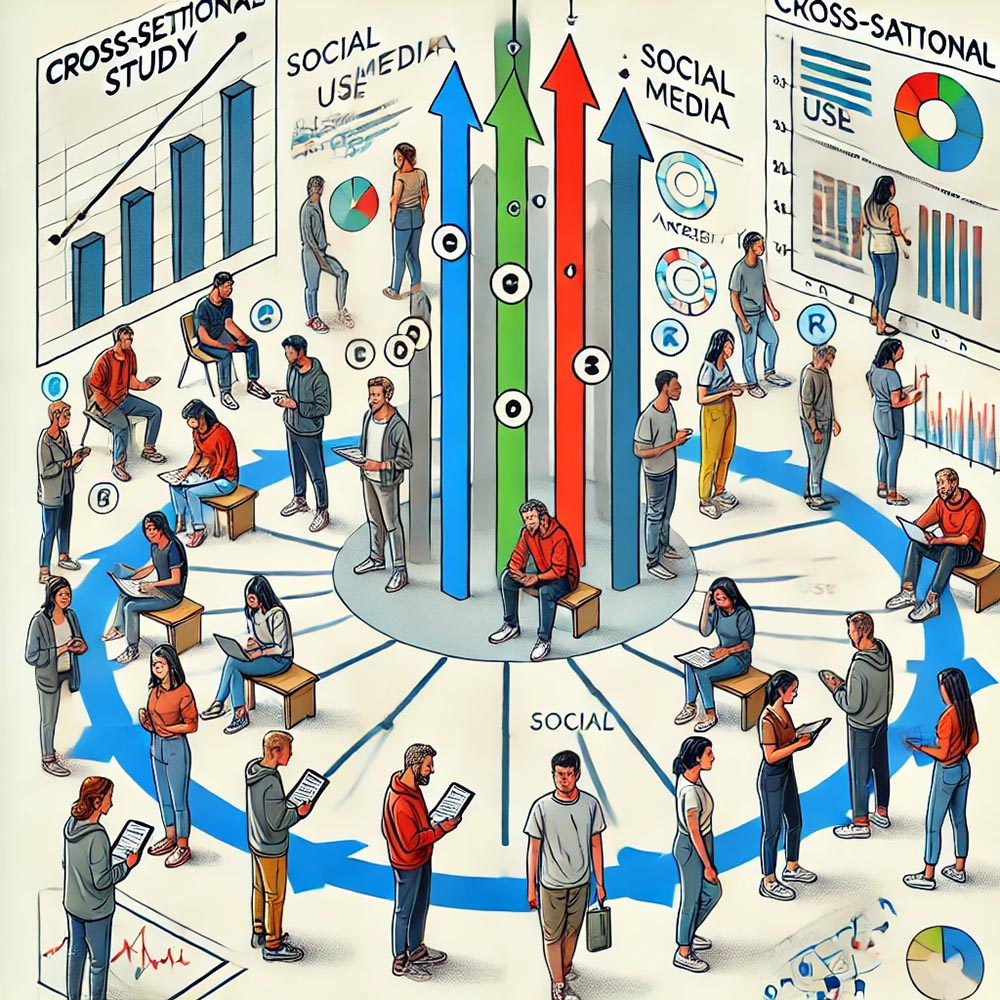
\includegraphics[width=1\textwidth,height=\textheight]{images/fig032.jpg}

\emph{Figure 032. A visual representation of a cross-sectional study. The image could depict a single point in time with a large group of diverse participants responding to a survey. Arrows might show the relationships being studied, such as the link between social media use and anxiety levels. This visual would help students understand the nature of cross-sectional designs and their focus on capturing data at one moment.}

In contrast, \textbf{longitudinal designs} involve observing the same participants over an extended period. By tracking changes in the same group of individuals over time, researchers can study developments, trends, and causal relationships more effectively than with cross-sectional designs. For example, you might follow a group of participants over several years to study the impact of media exposure on their political attitudes. By collecting data at multiple points in time, longitudinal studies allow you to see how variables evolve and how earlier events or exposures might influence later outcomes.

Longitudinal designs are particularly valuable for studying changes and developments that occur over time. They can provide insights into long-term effects and help establish causality by showing how one variable influences another across different time points. For instance, a longitudinal study might reveal that increased media exposure during adolescence leads to changes in political attitudes during adulthood, providing evidence of a causal relationship.

However, longitudinal research also presents several challenges. One of the most significant is participant dropout, also known as attrition. Over the course of a long-term study, some participants may drop out due to various reasons, such as losing interest, moving away, or experiencing life changes that make continued participation difficult. This can lead to biased results if the individuals who remain in the study differ in important ways from those who drop out. Additionally, longitudinal studies are typically more time-consuming and costly than cross-sectional studies, requiring careful planning and sustained resources.

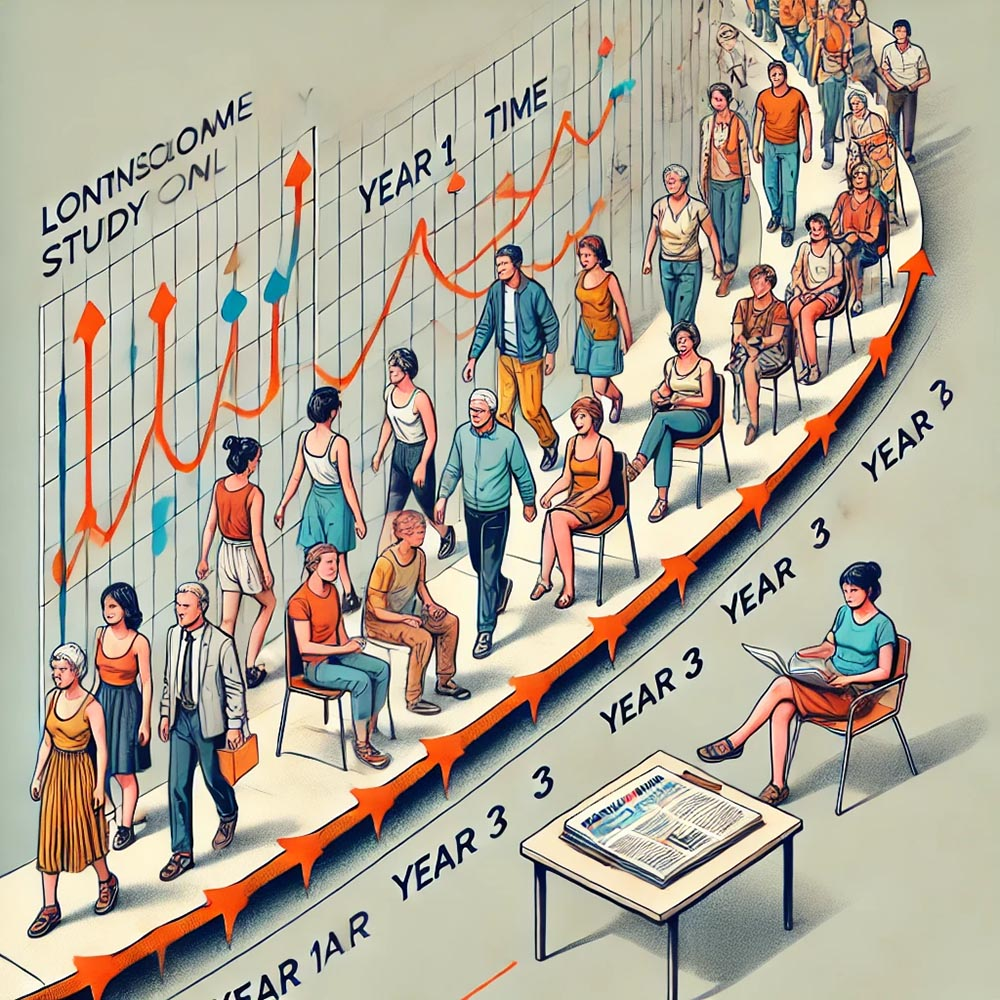
\includegraphics[width=1\textwidth,height=\textheight]{images/fig033.jpg}

\emph{Figure 033. A timeline illustrating a longitudinal study. The image could show a group of participants being observed at multiple time points (e.g., Year 1, Year 3, Year 5), with arrows indicating how data is collected and tracked over time. The visual could highlight the concept of tracking changes and developments in variables, such as political attitudes, across these time points. This image would help students visualize the extended nature of longitudinal designs and their ability to capture change.}

In the classroom, we will discuss the advantages and limitations of cross-sectional designs. Through examples and case studies, you will explore how these designs are used in real-world research, particularly in mass media studies. You will also have the opportunity to analyze a dataset from a cross-sectional study, interpreting the findings and considering how the design influences the conclusions that can be drawn.

We will also delve into longitudinal studies by examining famous examples, such as long-term media effect studies that have tracked changes in media consumption and its impact on behavior and attitudes over decades. These discussions will help you understand the value of longitudinal research in uncovering long-term trends and causal relationships.

To further your understanding, we will engage in a discussion on the challenges of longitudinal research, such as participant dropout. You will brainstorm potential solutions to these challenges, such as strategies for retaining participants or adjusting analyses to account for attrition. By the end of this section, you will be equipped to choose the appropriate non-experimental design for your research questions and to understand the implications of each approach for your findings.

By mastering both cross-sectional and longitudinal designs, you will be prepared to conduct research that is both insightful and methodologically sound, even when experimental manipulation is not possible. These non-experimental designs are essential tools in the researcher's toolkit, particularly in fields like mass media where long-term effects and broad population trends are often of interest.

\subsection{Sampling Methods}\label{sampling-methods}

In research, the method you use to select your sample can significantly impact the validity and generalizability of your findings. Sampling methods determine how participants are chosen from the larger population and are crucial in ensuring that your study accurately represents the group you intend to study. There are various sampling methods, each with its own advantages and limitations. Understanding these methods will help you make informed decisions about how to design your study and interpret your results.

One of the most effective and widely used sampling methods is \textbf{random sampling}. In random sampling, participants are selected in such a way that every member of the population has an equal chance of being chosen. This method is considered the gold standard in sampling because it minimizes selection bias and enhances the generalizability of your study results. For example, imagine you are conducting a survey to understand viewer preferences for television programs. By randomly selecting viewers from a television network's subscriber list, you ensure that each subscriber, regardless of their viewing habits, has an equal chance of being included in the study. This randomness helps ensure that your sample is representative of the larger population, allowing you to generalize your findings more confidently.

Random sampling is particularly valuable when you need to draw conclusions that apply broadly to the entire population. However, it requires careful planning and sometimes a larger sample size to ensure that the random selection truly reflects the diversity of the population. Additionally, while random sampling reduces bias, it does not eliminate it entirely; factors such as non-response can still introduce some degree of bias.

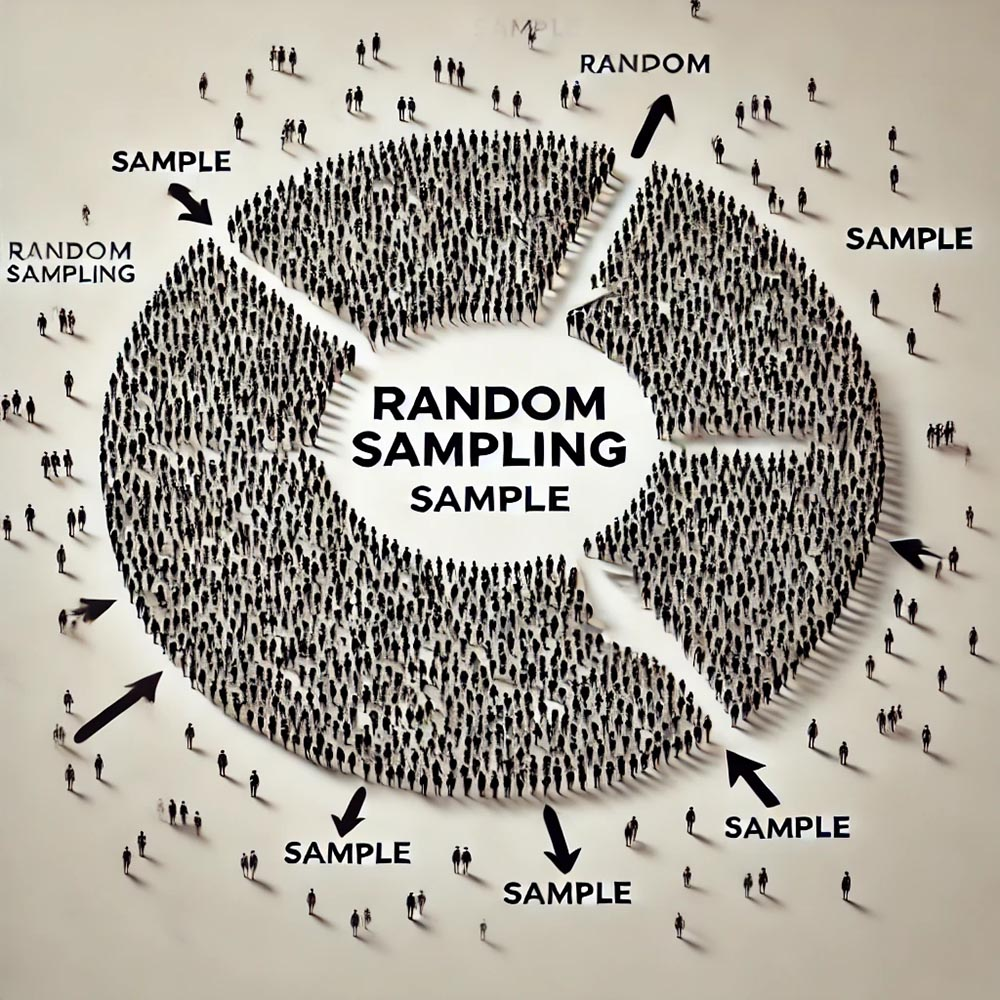
\includegraphics[width=1\textwidth,height=\textheight]{images/fig034.jpg}

\emph{Figure 034. A visual diagram showing the process of random sampling. The image could depict a large circle representing the entire population, with small dots inside representing individuals. Arrows could point from different parts of the population to a smaller circle labeled ``Sample,'' indicating that individuals are selected at random. This visual would help students understand how random sampling works and its role in ensuring representativeness.}

Another method is \textbf{stratified sampling}, which involves dividing the population into distinct subgroups, or strata, and then randomly sampling from each group. This approach ensures that each subgroup is represented in the sample, which is particularly useful when certain characteristics (such as age, gender, or income level) are important for the research. For instance, if you are studying media preferences across different age groups, you might divide the population into age strata (e.g., 18-29, 30-49, 50+) and then randomly select participants from each age group. This way, you ensure that each age group is adequately represented in your sample, allowing for more precise comparisons between groups.

Stratified sampling is especially beneficial when the population is heterogeneous, meaning that there are significant differences between subgroups. By ensuring that each subgroup is proportionately represented, stratified sampling improves the accuracy of your estimates and reduces sampling error. However, it also requires more detailed knowledge of the population and can be more complex to implement than simple random sampling.

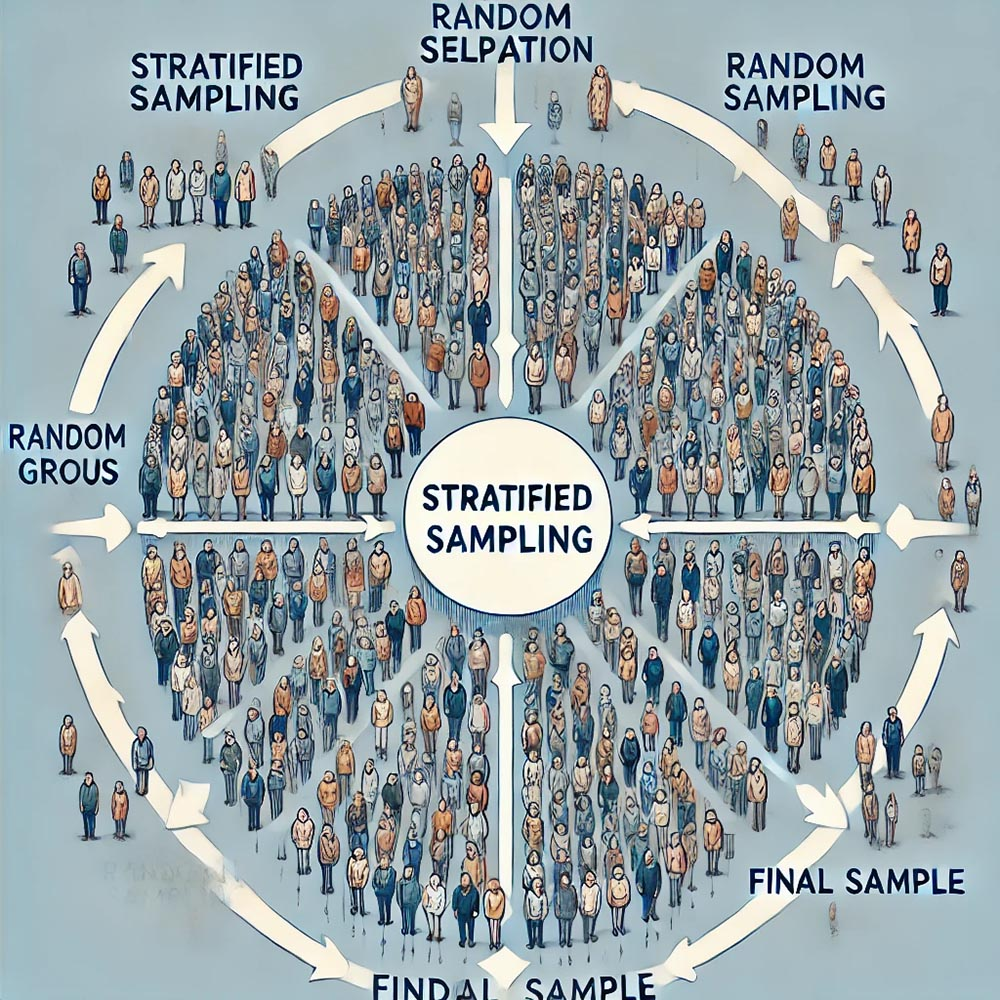
\includegraphics[width=1\textwidth,height=\textheight]{images/fig035.jpg}

\emph{Figure 035. An illustration of stratified sampling. The image could show a large population divided into several subgroups (e.g., different age groups), with arrows indicating random selection from each subgroup into the final sample. This visual would help students visualize how stratified sampling ensures representation from all relevant subgroups.}

In contrast, \textbf{convenience sampling} involves selecting participants who are readily available and easy to recruit. While this method is often used because of its practicality, it comes with significant limitations in terms of representativeness and generalizability. For example, if you are studying media habits among students and decide to survey students in your classroom, you are using convenience sampling. While this approach is easy and cost-effective, the sample may not be representative of all students or of the general population, leading to potential biases in your findings.

Convenience sampling is often used in exploratory research, pilot studies, or situations where other sampling methods are not feasible. However, it is crucial to recognize its limitations. Since the sample is not randomly selected, the results may not be generalizable beyond the specific group studied. To mitigate some of these drawbacks, researchers can combine convenience sampling with other techniques, such as increasing the sample size or using quota sampling to ensure some level of diversity within the sample.

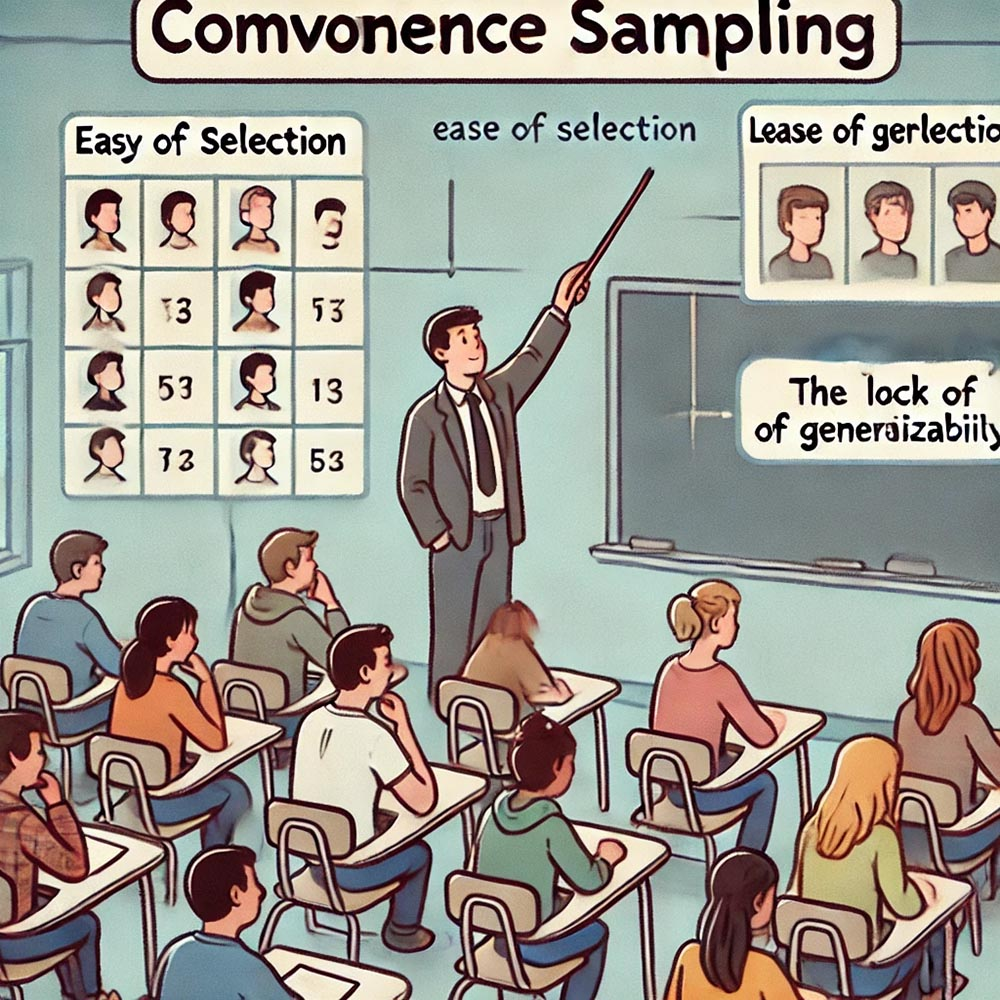
\includegraphics[width=1\textwidth,height=\textheight]{images/fig036.jpg}

\emph{Figure 036. A simple diagram showing convenience sampling. The image could depict a researcher standing in front of a classroom, selecting participants from the students present, with a text box highlighting the ease of selection but also noting the lack of generalizability. This visual would help students understand the trade-offs involved in convenience sampling.}

In the classroom, we will explore these sampling methods through practical examples and activities. For random sampling, we will discuss real-world cases where this method was used to enhance the validity of the research findings. You will also participate in a classroom activity where you create a simple random sampling plan for a hypothetical study, helping you grasp the practical application of this method.

We will also delve into stratified sampling by having you design a stratified sampling plan for a research project. This exercise will involve determining the appropriate strata and deciding how to sample from each subgroup to ensure a representative sample. This hands-on approach will solidify your understanding of how to implement stratified sampling in your own research.

Finally, we will discuss the practical benefits and limitations of convenience sampling. You will be assigned to identify situations where convenience sampling might be the only feasible method and to discuss ways to mitigate its drawbacks. By understanding when and how to use convenience sampling, you will be better prepared to make informed decisions about your research design.

By mastering these sampling methods, you will be equipped to select the most appropriate method for your research questions and to understand the implications of each method for your findings. This knowledge is essential for conducting rigorous and credible research, whether in mass media studies or other fields.

\section{Data Collection Techniques}\label{data-collection-techniques}

\subsection{Surveys and Questionnaires}\label{surveys-and-questionnaires}

Surveys and questionnaires are among the most common tools used in research to gather data from a large number of participants efficiently. These tools allow researchers to collect information on attitudes, behaviors, preferences, and other variables of interest. However, the design of survey questions is crucial to ensure that the data collected is accurate, meaningful, and reflective of the respondents' true opinions. Understanding the different types of survey questions---such as Likert-type items, closed-ended questions, and open-ended questions---will equip you with the skills to design effective surveys for your research.

One of the most widely used types of survey questions is the \textbf{Likert-type item}. A Likert-type item is a statement to which respondents indicate their level of agreement on a scale, typically ranging from ``strongly disagree'' to ``strongly agree.'' For example, you might ask respondents to rate their agreement with the statement, ``Social media has a positive impact on society,'' using a scale from 1 (strongly disagree) to 5 (strongly agree). This type of question is particularly useful for measuring attitudes and opinions because it provides a clear, quantifiable way to capture the strength of respondents' feelings on an issue.

Likert-type items are advantageous because they offer a simple and standardized way to measure complex attitudes, allowing for easy comparison across respondents. Additionally, because the scale is consistent across items, Likert-type questions can be used to create composite scores that reflect overall attitudes toward a topic. However, careful attention must be paid to the wording of the statements to avoid bias. For instance, a poorly worded statement could lead respondents to answer in a way that does not accurately reflect their true opinions.

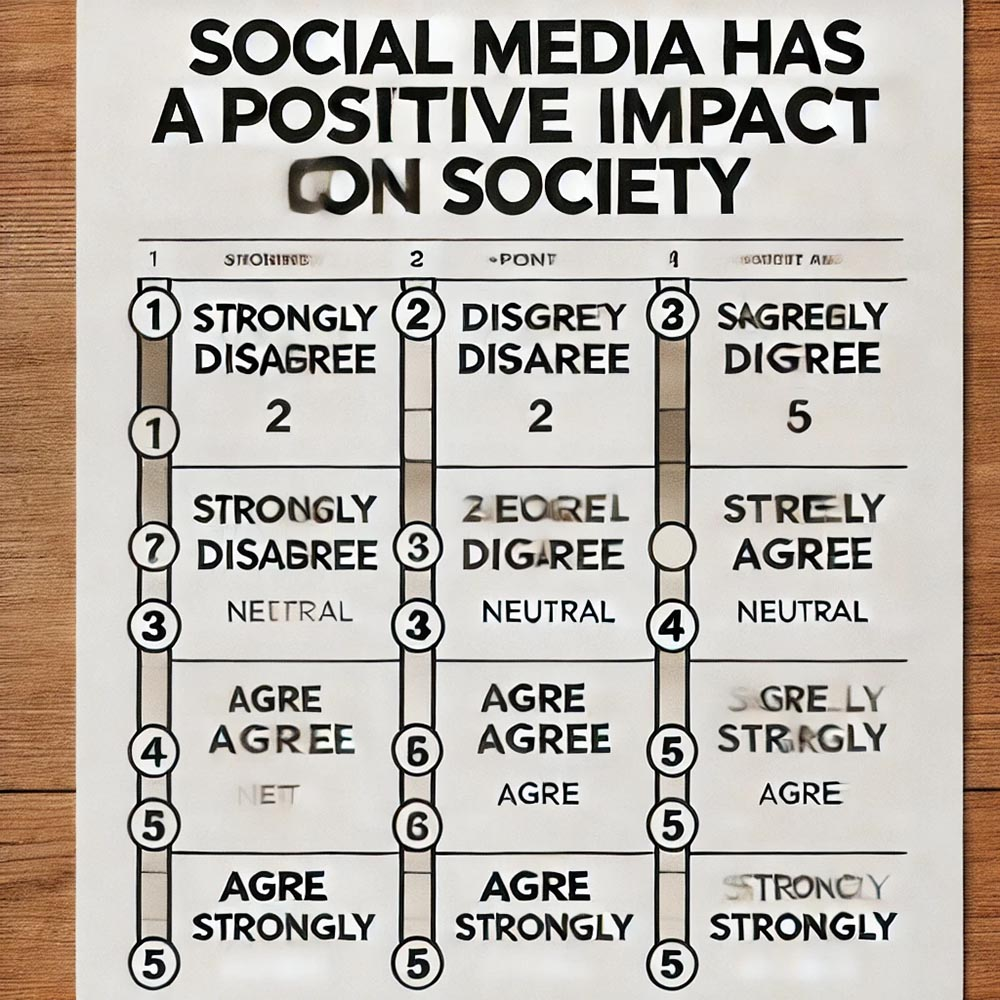
\includegraphics[width=1\textwidth,height=\textheight]{images/fig037.jpg}

\emph{Figure 037. An example of a Likert scale question. The image could show the statement ``Social media has a positive impact on society'' with a five-point scale ranging from 1 (Strongly Disagree) to 5 (Strongly Agree). Each point on the scale could be labeled to emphasize the gradation of agreement. This visual would help students understand how Likert-type items are structured and how they are used to measure attitudes.}

In our classroom discussions, we will explore examples from existing surveys to see how Likert-type items are employed effectively. You will also have the opportunity to create your own Likert-type items based on a research question of your choice. This exercise will be followed by a class discussion on the importance of clear and unbiased wording in survey design, helping you refine your skills in crafting effective survey questions.

Another common type of survey question is the \textbf{closed-ended question}. Closed-ended questions provide respondents with a set of predefined responses to choose from. For example, you might ask, ``How often do you use social media?'' with response options like ``Daily,'' ``Weekly,'' ``Monthly,'' or ``Never.'' Closed-ended questions are highly efficient for collecting data because they are easy to answer, straightforward to analyze, and allow for quick comparisons across different respondents.

The main advantage of closed-ended questions is their simplicity and ease of analysis. Since the responses are predefined, you can quickly categorize and quantify the data, making it easier to identify patterns and trends. However, one limitation of closed-ended questions is that they may constrain respondents' answers, potentially leading to a loss of nuanced information. For instance, if the predefined options do not fully capture the respondents' true behaviors or opinions, the data collected may not be entirely accurate.

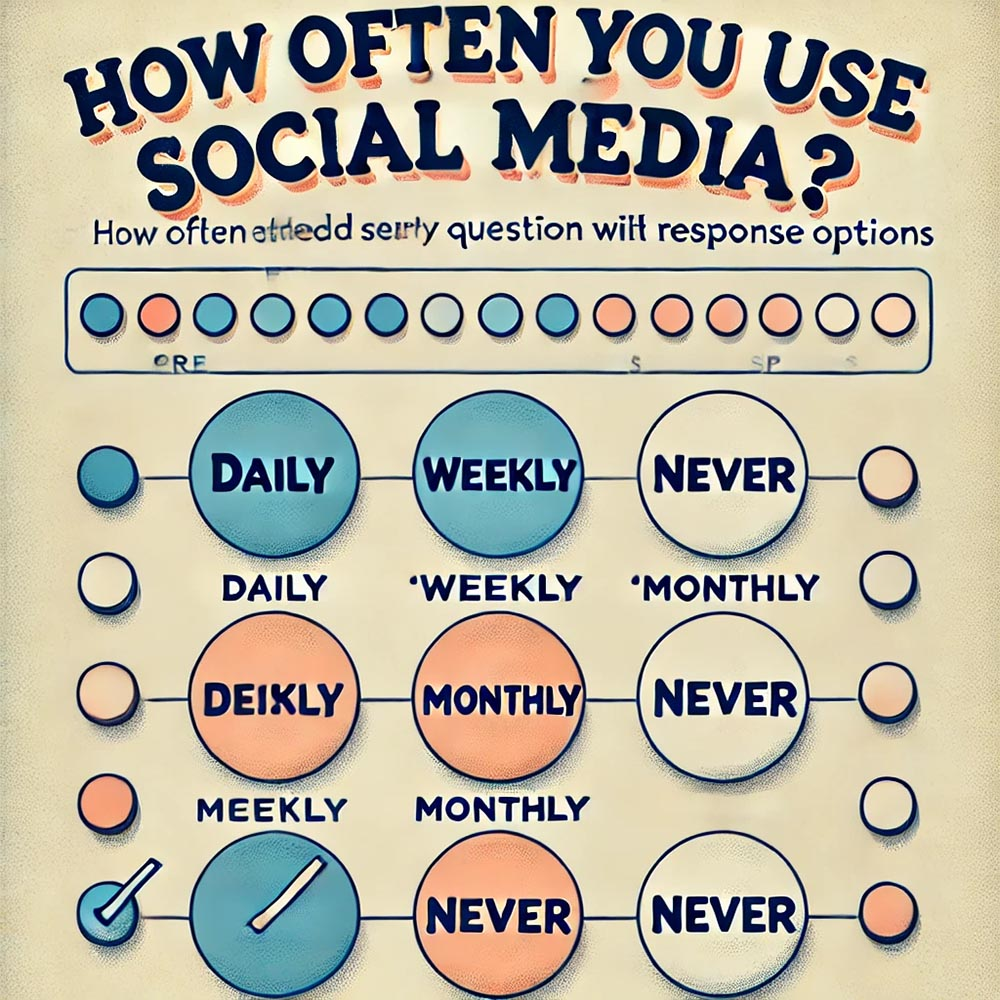
\includegraphics[width=1\textwidth,height=\textheight]{images/fig038.jpg}

\emph{Figure 038. A sample closed-ended question with response options. The image could show the question ``How often do you use social media?'' followed by the options ``Daily,'' ``Weekly,'' ``Monthly,'' and ``Never.'' The visual could highlight how the predefined responses make it easy to quantify and analyze the data. This visual would help students understand the structure of closed-ended questions and their advantages in survey design.}

To deepen your understanding, we will discuss the advantages and limitations of closed-ended questions, particularly in terms of how they affect the richness and accuracy of the data collected. You will engage in designing closed-ended questions for a survey, and we will discuss potential biases in the answer choices. This discussion will help you consider how the framing of questions and the selection of response options can influence the results of your survey.

In contrast to closed-ended questions, \textbf{open-ended questions} allow respondents to answer in their own words, providing richer and more detailed data. For example, you might ask, ``What do you think is the most significant impact of social media on society?'' This type of question gives respondents the freedom to express their thoughts and opinions without being confined to predefined responses.

Open-ended questions are valuable because they can uncover insights that might be missed with closed-ended questions. They allow respondents to provide more nuanced and personal responses, which can reveal underlying attitudes, motivations, or concerns. However, the trade-off is that open-ended questions can be more challenging to analyze. Since responses are often varied and complex, coding and interpreting the data requires careful consideration and may be time-consuming.

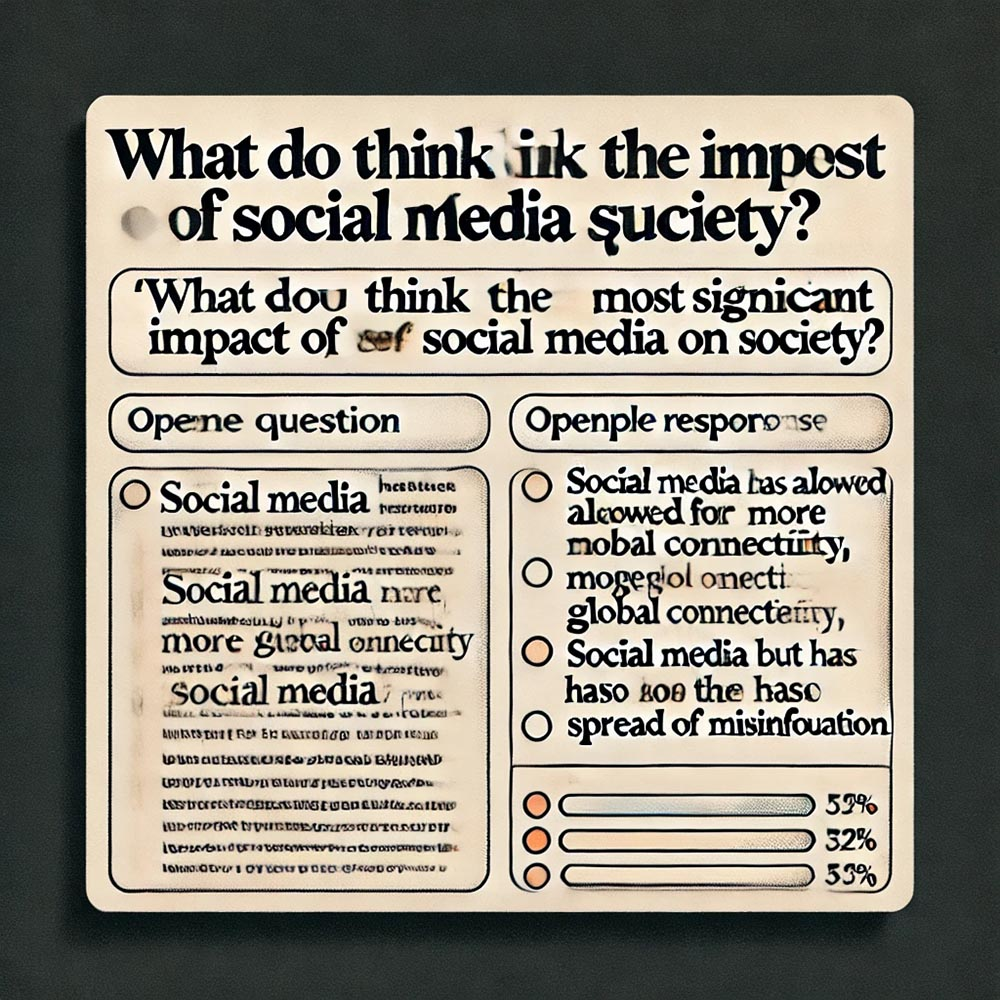
\includegraphics[width=1\textwidth,height=\textheight]{images/fig039.jpg}

\emph{Figure 039. An illustration of an open-ended question response. The image could show the question ``What do you think is the most significant impact of social media on society?'' with a blank space for respondents to write their answers. The visual could also include a snippet of a sample response, highlighting the depth and richness of the data collected through open-ended questions. This visual would help students appreciate the value of open-ended questions in capturing detailed and nuanced information.}

In our lessons, we will illustrate how open-ended questions can uncover insights that closed-ended questions might miss. You will be assigned a task where you analyze responses from open-ended questions, identifying common themes and discussing the challenges in coding the data. This exercise will help you understand the strengths and limitations of open-ended questions and develop your skills in qualitative data analysis.

By mastering the use of Likert-type items, closed-ended questions, and open-ended questions, you will be well-equipped to design surveys and questionnaires that effectively gather the information you need for your research. Understanding the appropriate context for each type of question and the implications for data analysis is essential for conducting rigorous and insightful research in the field of mass communications.

\subsection{Observation Methods}\label{observation-methods}

Observation methods are a key component of qualitative research, particularly when studying behaviors, interactions, and environments in their natural settings. Unlike surveys or experiments, which often involve some degree of control or intervention, observation methods allow researchers to gather data in a more organic and unstructured way. There are various observation methods, each with its own approach to the research process. Understanding these methods---such as participant observation, complete observation, and direct observation---will enhance your ability to design and conduct qualitative research that captures the complexity of human behavior.

\textbf{Participant observation} is a method where the researcher actively engages in the environment or group being studied while simultaneously observing behaviors. This method is particularly useful when studying social interactions and cultural practices because it allows the researcher to gain a deeper, insider's perspective. For example, a researcher might join an online forum dedicated to discussing news events to observe how users interact and share information. By becoming a participant in the forum, the researcher can experience the dynamics of the group firsthand and gain insights that might not be accessible through more detached observation methods.

However, participant observation comes with its own set of challenges, particularly related to ethical considerations and the potential for observer bias. As a participant, the researcher's presence and actions can influence the behavior of those being observed, known as the observer effect. Additionally, the researcher's own beliefs and experiences may color their observations, leading to bias in the data collection process. To address these challenges, it is important to maintain a balance between engagement and objectivity, and to be aware of how your participation might affect the data.

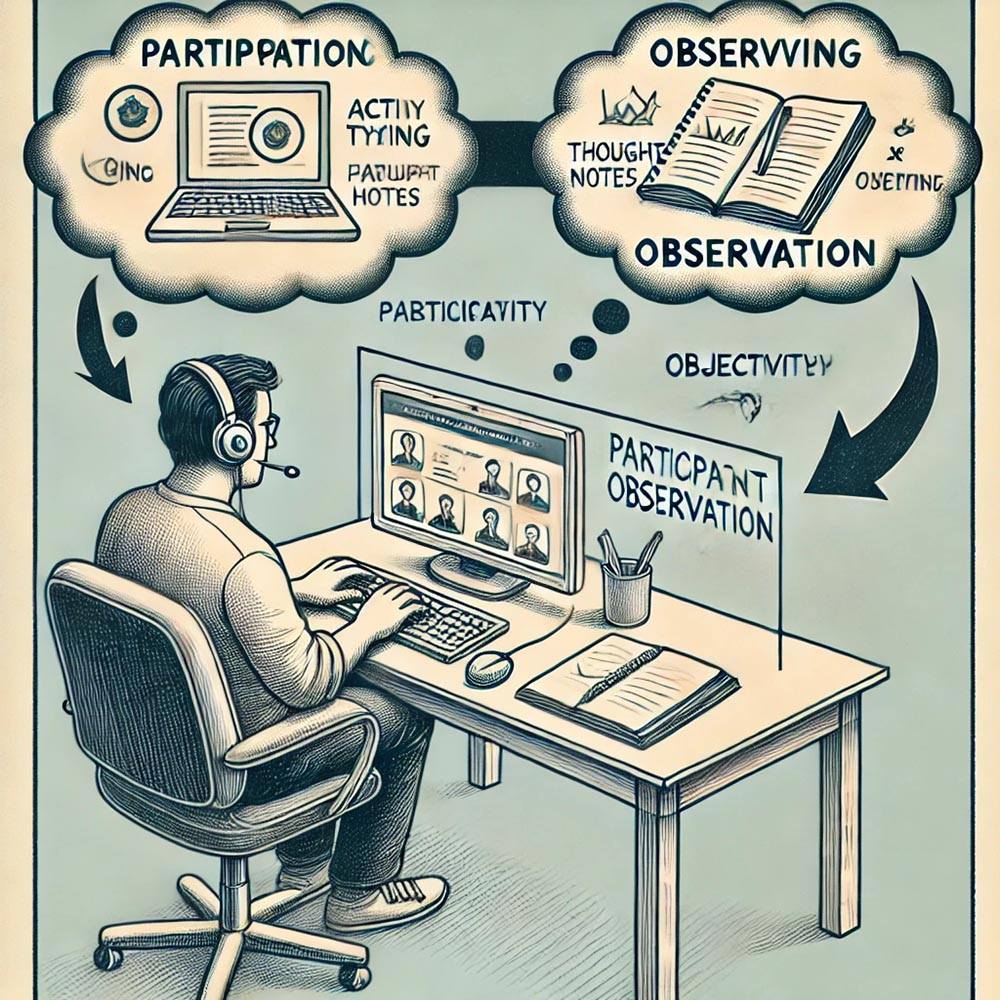
\includegraphics[width=1\textwidth,height=\textheight]{images/fig040.jpg}

\emph{Figure 040. A diagram illustrating participant observation in action. The image could depict a researcher sitting at a computer, engaged in an online forum discussion, with a thought bubble showing them taking notes on the interaction. Arrows might indicate the dual roles of participating and observing, emphasizing the challenge of maintaining objectivity. This visual would help students understand the unique aspects of participant observation and the complexities involved in this method.}

In our classroom discussions, we will explore the ethical considerations and challenges of participant observation. We will engage in a simulation where you will role-play as participant observers in a hypothetical scenario, allowing you to experience firsthand the difficulties of balancing participation with observation. After the simulation, we will reflect on these experiences and discuss how to mitigate potential biases in your research.

On the other end of the spectrum is the \textbf{complete observer} method, where the researcher observes the environment without interacting or participating in it. This approach minimizes the researcher's influence on the subjects being studied, as the participants are often unaware that they are being observed. For example, you might conduct a study where you observe interactions in a public place, such as a park or café, without engaging with the people you are observing. By maintaining a distance, you can capture behaviors as they naturally occur, reducing the risk of altering the dynamics of the environment.

While the complete observer role reduces the risk of the observer effect, it also comes with limitations. One of the main drawbacks is the potential for a lack of depth in the data collected. Since the researcher does not engage with the participants, they may miss out on the context or motivations behind certain behaviors. Additionally, this method can lead to ethical concerns, particularly regarding the right to privacy and informed consent, especially in settings where participants are unaware that they are being observed.

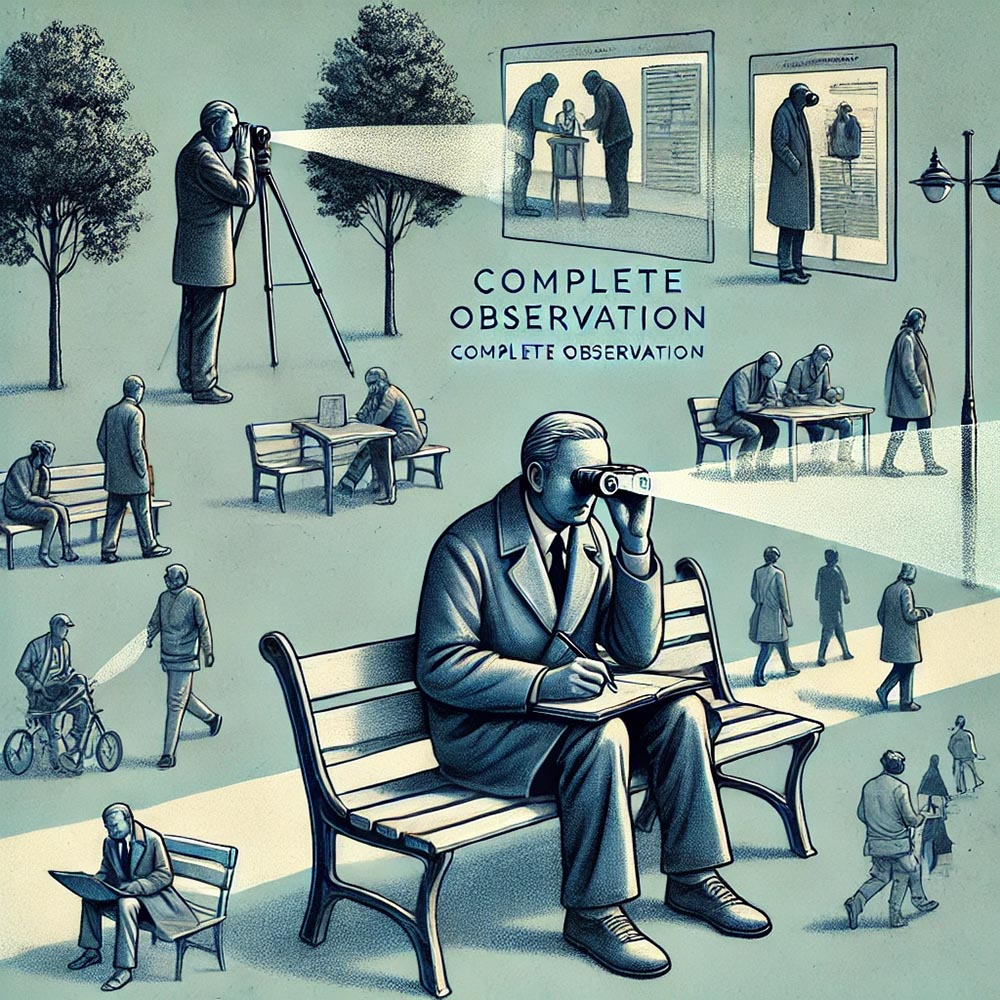
\includegraphics[width=1\textwidth,height=\textheight]{images/fig041.jpg}

\emph{Figure 041. An illustration of a researcher conducting complete observation. The image could show a researcher sitting discreetly in a public place, such as a park bench, taking notes on the interactions they observe without engaging with the participants. The visual might highlight the unobtrusive nature of complete observation, while also noting potential ethical concerns. This image would help students grasp the concept of complete observation and its implications for research.}

To help you understand the complete observer role, we will discuss its pros and cons, particularly in relation to the richness of the data and the potential for ethical issues. You will be assigned to perform a complete observation in a real or simulated environment, after which you will report your findings. This exercise will give you practical experience in observing without intervening, helping you develop the skills needed to conduct complete observations effectively.

\textbf{Direct observation} is another method that involves systematically watching and recording behaviors or events as they naturally occur. Unlike participant observation, where the researcher engages with the environment, or complete observation, where the researcher remains detached, direct observation focuses on the systematic and structured recording of specific behaviors. For example, you might conduct a study where you observe and record the frequency of certain types of media consumption in a public space, such as how often people check their phones while sitting in a café.

Direct observation is particularly useful for studies that require precise and quantifiable data on specific behaviors. It allows researchers to collect data that is directly observable, reducing the reliance on self-reported information, which can sometimes be inaccurate or biased. However, the challenge with direct observation is maintaining consistency in how behaviors are recorded and ensuring that the observation process does not become intrusive or influence the behaviors being studied.

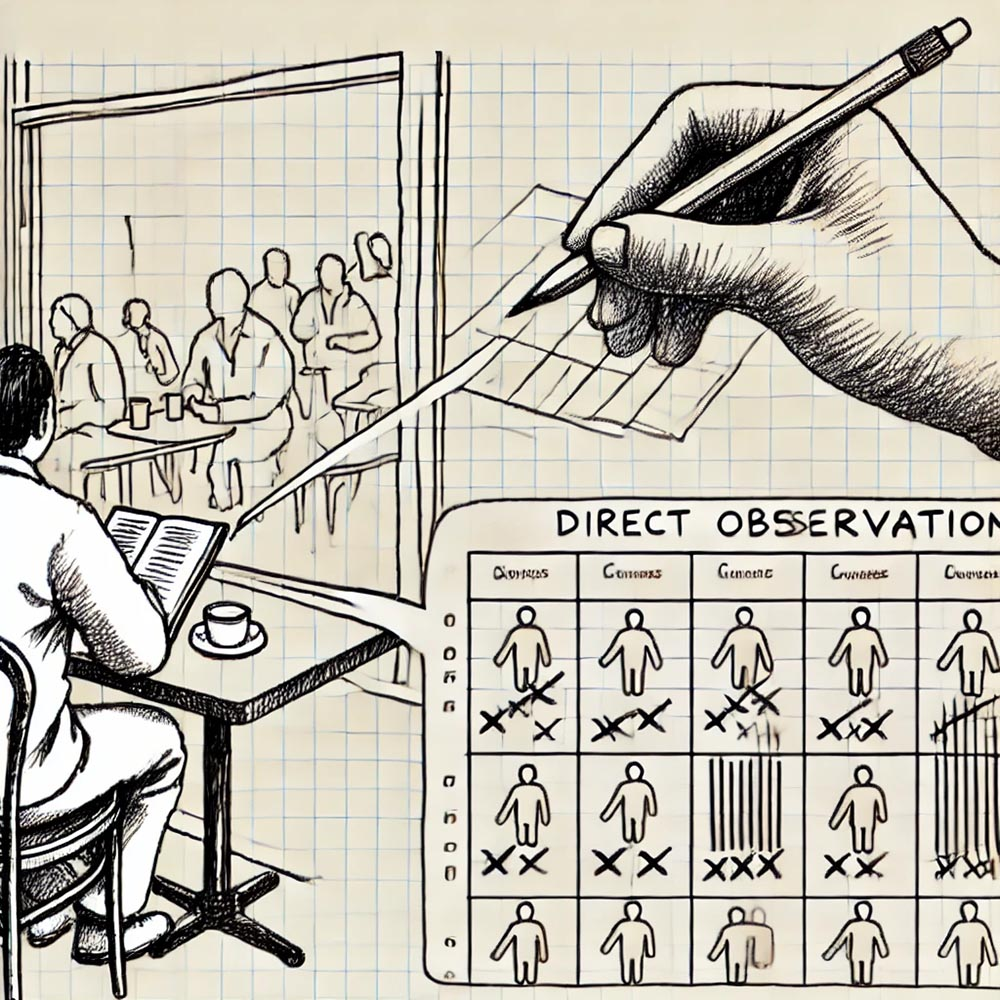
\includegraphics[width=1\textwidth,height=\textheight]{images/fig042.jpg}

\emph{Figure 042. A chart or grid used by a researcher during direct observation. The image could show a researcher systematically recording behaviors, such as phone usage in a café, using a tally or checklist. The visual might highlight the structured nature of direct observation and the importance of consistency in recording data. This image would help students understand how direct observation is conducted and the attention to detail required for this method.}

In our lessons, we will provide examples where direct observation has been effectively used in media research, such as studies on media consumption patterns or public behavior in response to media stimuli. You will participate in a direct observation exercise, where you will observe and record specific behaviors in a given environment. After the exercise, we will discuss the challenges you faced, such as maintaining objectivity and consistency in your observations, and how these challenges can be addressed in your research.

By mastering these observation methods---participant observation, complete observation, and direct observation---you will be equipped to choose the most appropriate method for your research questions and to conduct qualitative research that captures the complexity of human behavior. Each method offers unique insights and challenges, and understanding when and how to use them will enhance your ability to gather meaningful and reliable data in your studies.

\subsection{Content Analysis}\label{content-analysis}

Content analysis is a research method used to systematically analyze media content by breaking down the communication into categories and examining the presence, meanings, and relationships of certain words, themes, or concepts. This method is particularly useful in mass media research for studying patterns, trends, and the influence of media messages on audiences. Content analysis can be divided into two main types: manifest content analysis, which focuses on the tangible and observable elements of the content, and latent content analysis, which delves into the underlying meanings and themes that are not immediately obvious.

\textbf{Manifest content} refers to the explicit, surface-level elements of media content that can be directly observed and quantified. This might include the frequency of certain words, phrases, or images in a text. For example, you could conduct a manifest content analysis to count the number of times the phrase ``climate change'' appears in news articles over a specified period. By quantifying these occurrences, you can identify trends in how often certain topics are covered or how frequently specific terms are used in the media.

Manifest content analysis is advantageous because it provides clear, objective data that can be easily replicated and compared across different studies. However, it is important to remember that while manifest content analysis can tell you what is present in the media, it does not necessarily explain the deeper meanings or implications behind the content. For instance, knowing that ``climate change'' is mentioned frequently does not reveal whether the coverage is positive, negative, or neutral, or what underlying messages are being conveyed.

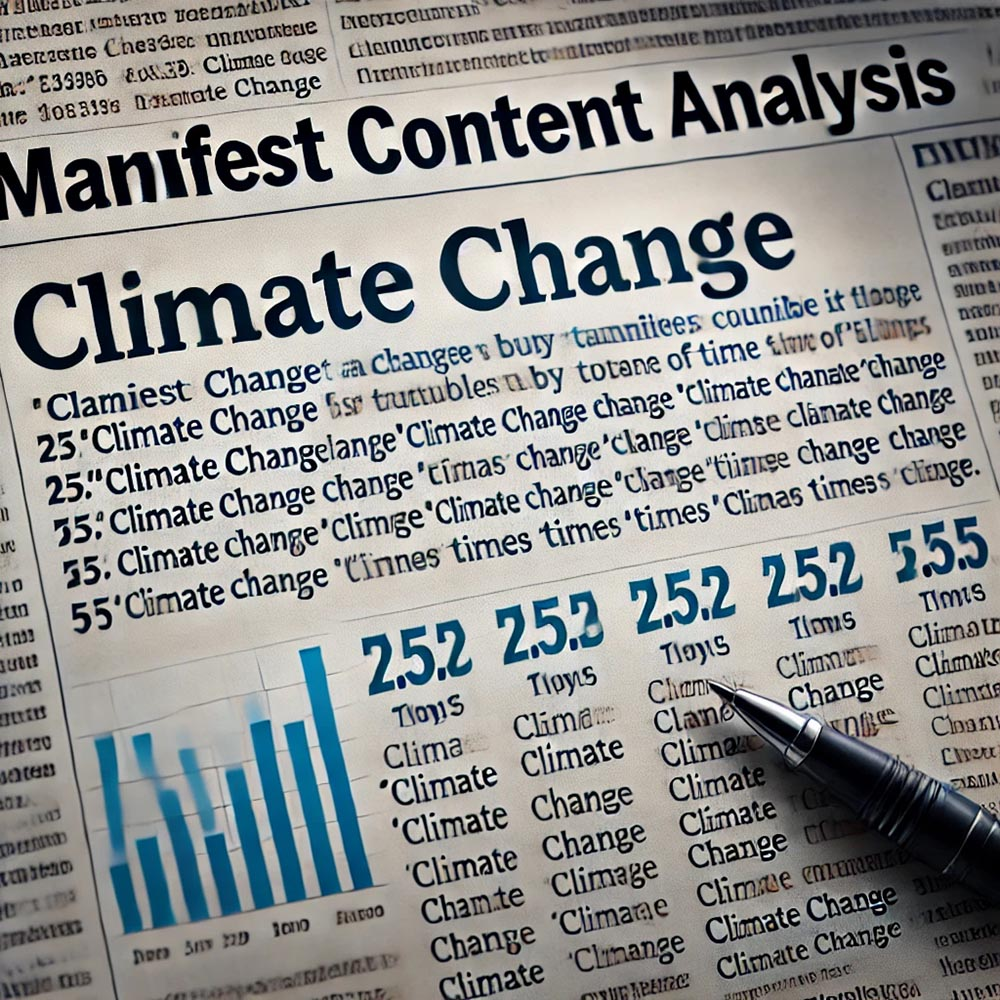
\includegraphics[width=1\textwidth,height=\textheight]{images/fig043.jpg}

\emph{Figure 043. A screenshot of a news article with the word ``climate change'' highlighted each time it appears. This visual could include a tally at the side showing the total count, illustrating how manifest content analysis quantifies observable elements in media content. This image would help students understand how manifest content analysis focuses on counting tangible aspects of media.}

To help you grasp the application of manifest content analysis, we will explore examples from various media forms, such as newspapers, television broadcasts, and social media posts. You will have the opportunity to practice coding manifest content from a sample media text, where you will count and categorize specific elements, such as keywords or images. This exercise will also include a discussion on the importance of clear coding guidelines, which are essential to ensure consistency and accuracy in your analysis.

In contrast to manifest content, \textbf{latent content} refers to the underlying meanings, themes, or messages embedded within media content. Latent content analysis goes beyond the surface to explore the deeper significance of the content, such as the tone, bias, or ideological perspectives that may not be immediately apparent. For example, when analyzing a news article about political events, you might examine the underlying tone or bias of the coverage---whether it subtly favors one political party over another or presents the events in a positive or negative light.

Identifying and interpreting latent content is more complex than analyzing manifest content because it involves subjective judgment and interpretation. The same piece of content might be interpreted differently by different researchers, which can lead to variability in the findings. For this reason, latent content analysis often requires a more nuanced approach, including a thorough understanding of the context in which the content was produced and consumed.

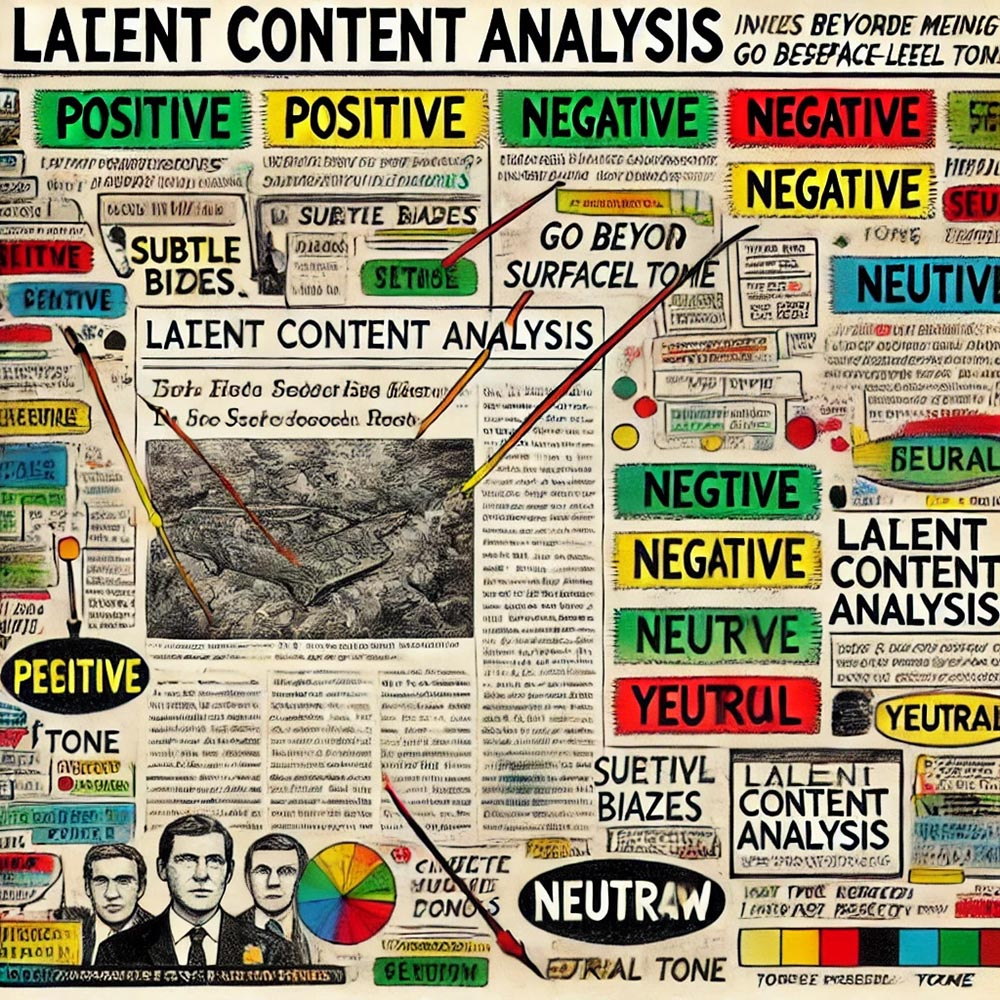
\includegraphics[width=1\textwidth,height=\textheight]{images/fig044.jpg}

\emph{Figure 044. A news article with color-coded highlights indicating different tones (e.g., positive, negative, neutral) and annotations pointing out subtle biases or underlying themes. This visual would help students see how latent content analysis requires interpretation beyond just counting words or phrases. The image could also include a legend explaining the color-coding used in the analysis.}

We will discuss the complexities of identifying and interpreting latent content through case studies, where you will analyze media samples to uncover hidden themes or biases. You will participate in a group activity designed to identify latent themes in a media sample, followed by a discussion on the subjectivity of such analysis. This exercise will help you appreciate the challenges and intricacies of latent content analysis, as well as the critical thinking required to conduct it effectively.

Central to both manifest and latent content analysis is the process of \textbf{coding}. Coding involves categorizing and tagging content to identify patterns, themes, or trends within qualitative data. Coding is essential because it allows you to systematically organize and interpret large amounts of data, making it easier to draw meaningful conclusions from your analysis. For example, you might develop a coding scheme to tag different types of media content as ``informative,'' ``persuasive,'' or ``entertainment.'' By applying this coding scheme to a sample of media texts, you can analyze the prevalence and distribution of these content types across different platforms or time periods.

Developing a coding scheme is a critical step in content analysis, as it defines how you will categorize and interpret the data. A well-defined coding scheme should be clear, consistent, and applicable across different texts. Additionally, achieving inter-coder reliability---where multiple researchers independently code the same content and reach similar conclusions---is essential to ensure the validity of your findings.

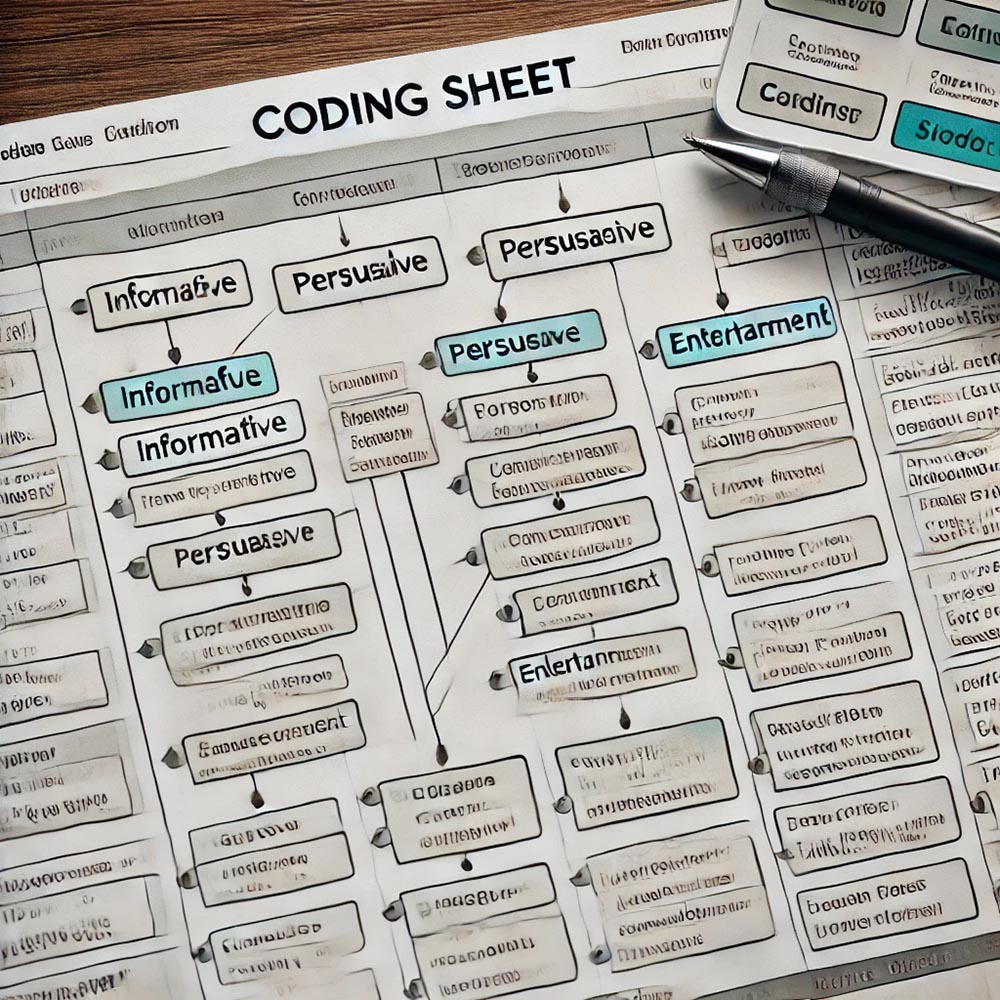
\includegraphics[width=1\textwidth,height=\textheight]{images/fig045.jpg}

\emph{Figure 045. A coding sheet or software interface showing a list of categories (e.g., ``informative,'' ``persuasive,'' ``entertainment'') with examples of how different media content is tagged under each category. This visual would help students understand how coding organizes content for analysis and the importance of having a well-defined coding scheme.}

In our lessons, you will learn how to develop a coding scheme by working on a project where you create one for a specific type of media, such as news articles, advertisements, or social media posts. You will then apply your coding scheme to a sample of content, analyzing the patterns that emerge. This hands-on project will conclude with a discussion of your findings and the challenges you encountered, such as ambiguities in the content or discrepancies in coding decisions.

By mastering the techniques of content analysis---including both manifest and latent content analysis and the coding process---you will be equipped to conduct rigorous and insightful research into media content. These skills will allow you to uncover the visible and hidden messages within media, contributing to a deeper understanding of how media shapes and reflects societal values, beliefs, and behaviors.

\chapter{Data Analysis and Statistical Techniques}\label{data-analysis-and-statistical-techniques}

\section{Descriptive Statistics}\label{descriptive-statistics}

\subsection{Measures of Central Tendency}\label{measures-of-central-tendency}

When analyzing data, it is essential to summarize the data set in a way that provides meaningful insights into the overall trends. Measures of central tendency---mean, median, and mode---are statistical tools that help us identify the central point around which the data tends to cluster. These measures offer different perspectives on what might be considered ``typical'' or ``average'' in a data set, and understanding how and when to use each one is crucial for effective data analysis.

The \textbf{mean} is one of the most commonly used measures of central tendency. It is calculated by adding together all the values in a data set and then dividing the sum by the number of values. The mean provides a straightforward and useful way to determine the average value in a data set. For example, if you wanted to calculate the average time spent on social media per day by a group of participants, you would sum up the total number of hours reported by all participants and then divide that sum by the number of participants. The result would give you the mean, or average, time spent on social media.

However, while the mean is useful, it is important to recognize its limitations. The mean is sensitive to outliers---values that are significantly higher or lower than the rest of the data. For instance, if most participants report spending 2 to 3 hours on social media daily, but one participant reports spending 12 hours, the mean will be skewed higher, potentially misrepresenting the typical social media usage for the group. In such cases, the mean might not accurately reflect the central tendency of the data.

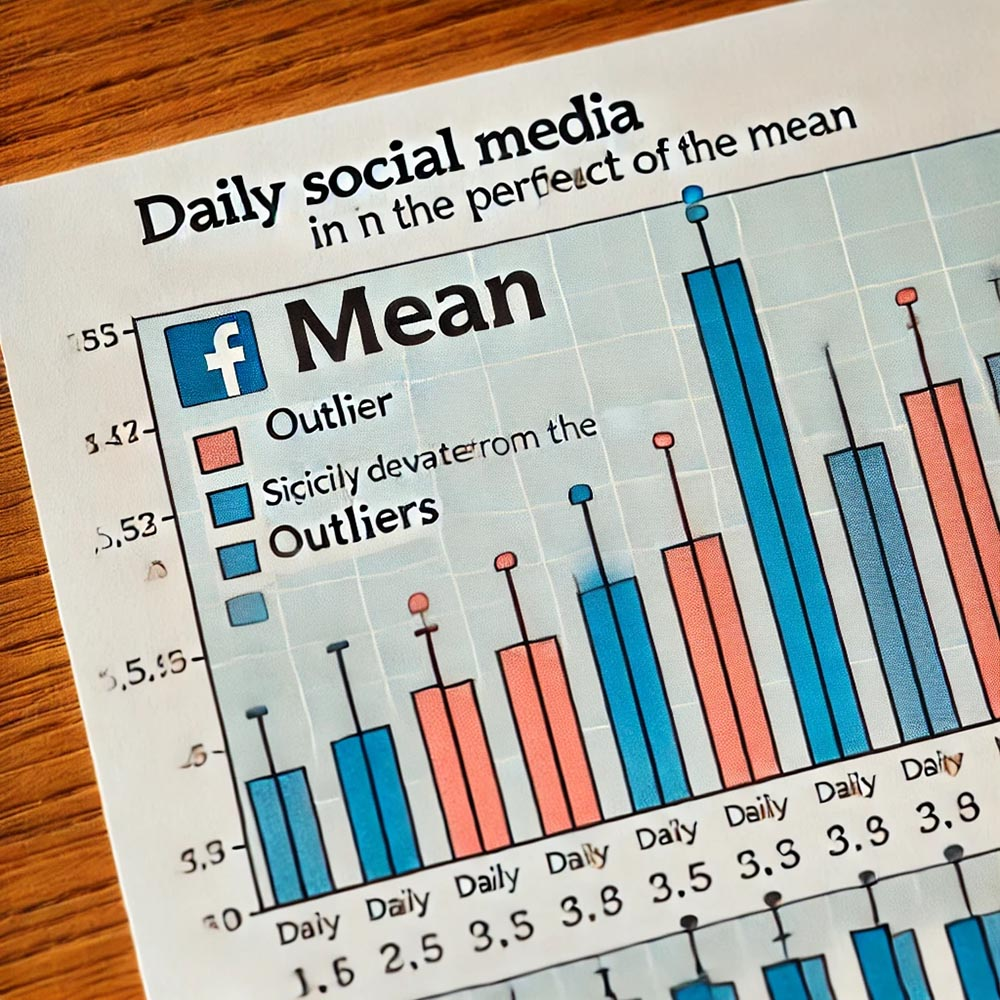
\includegraphics[width=1\textwidth,height=\textheight]{images/fig046.jpg}

\emph{Figure 046. A bar graph depicting the daily social media usage of a group of participants, with the mean highlighted by a horizontal line across the graph. The graph could include an outlier bar that significantly deviates from the others, visually illustrating how outliers can affect the mean. This image would help students understand the calculation and interpretation of the mean, especially in the presence of outliers.}

To further your understanding, we will use real-world examples to demonstrate how the mean is calculated and interpreted in various contexts. You will participate in a class exercise where you calculate the mean from a given dataset and then discuss situations where the mean may not be the best measure of central tendency, particularly when the data includes outliers.

The \textbf{median} is another measure of central tendency, representing the middle value in a data set when the values are arranged in ascending or descending order. If there is an even number of values, the median is calculated by averaging the two middle numbers. The median is particularly useful in skewed distributions, where the mean might be distorted by outliers. For example, if you wanted to find the median income of households in a particular city, you would list all household incomes in order and identify the middle value. The median provides a better representation of central tendency in cases where the data is not symmetrically distributed.

Unlike the mean, the median is not affected by outliers. In a skewed distribution, where a few extremely high or low values could distort the mean, the median offers a more accurate reflection of the typical value in the data set. For instance, in a city where a few households have exceptionally high incomes, the median income will give you a better sense of what the ``middle'' income is, rather than the mean, which could be inflated by the high-income outliers.

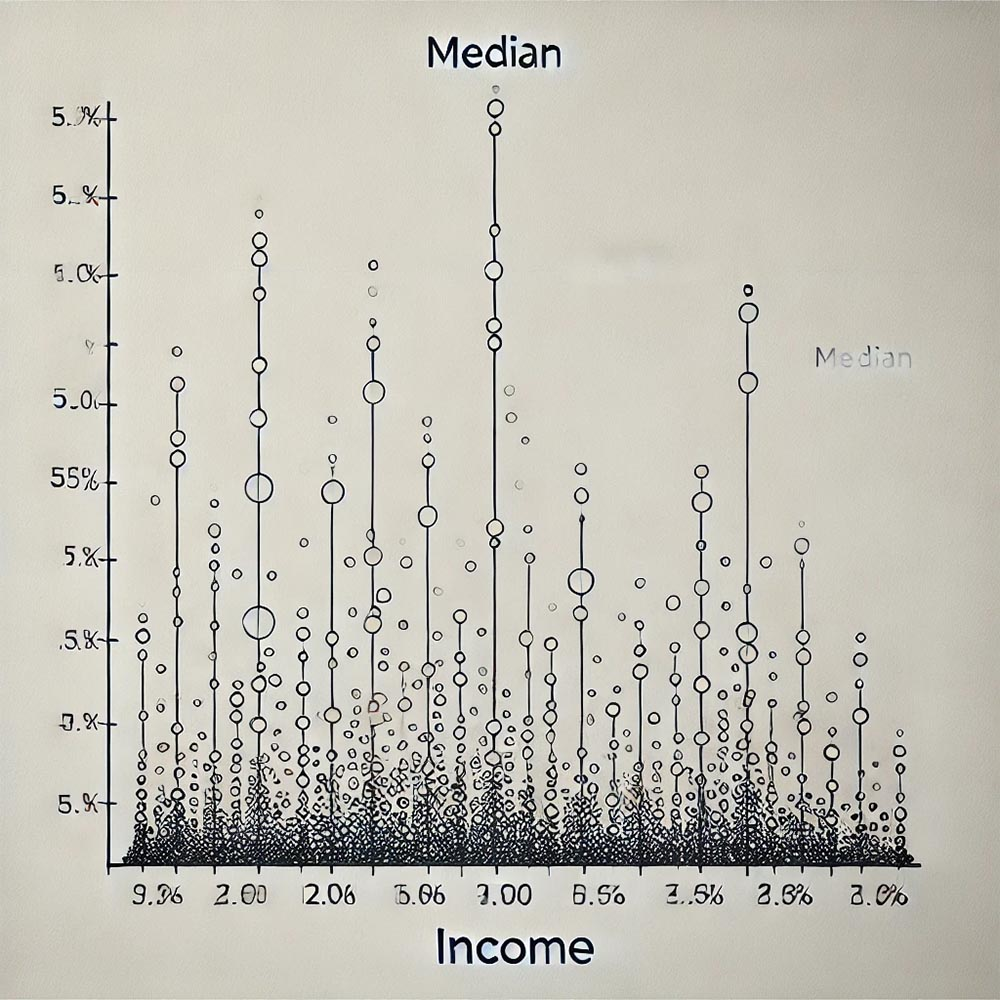
\includegraphics[width=1\textwidth,height=\textheight]{images/fig047.jpg}

\emph{Figure 047. A line plot or dot plot showing a series of income values arranged in order, with the median highlighted. The plot could show a few extreme values (outliers) at the higher end, demonstrating how the median remains unaffected by these outliers. This image would help students visualize how the median is calculated and why it is sometimes a better measure than the mean in skewed distributions.}

In class, we will explore examples of how the median can serve as a better measure of central tendency than the mean, especially in data sets with skewed distributions. You will calculate the median from a dataset provided and discuss its significance compared to the mean, considering when it might be more appropriate to use the median in your analyses.

The \textbf{mode} is the measure of central tendency that identifies the most frequently occurring value in a data set. Unlike the mean and median, which are based on mathematical calculations, the mode is simply the value that appears most often. For example, if you were to survey a group of people about their favorite news source and the most common response was ``CNN,'' then ``CNN'' would be the mode of that data set.

The mode is particularly useful when dealing with categorical data, where the data points are divided into distinct categories. It helps identify the most popular or common category in the data. For instance, in a survey asking participants to choose their preferred social media platform, the mode would reveal the platform that the majority of respondents prefer.

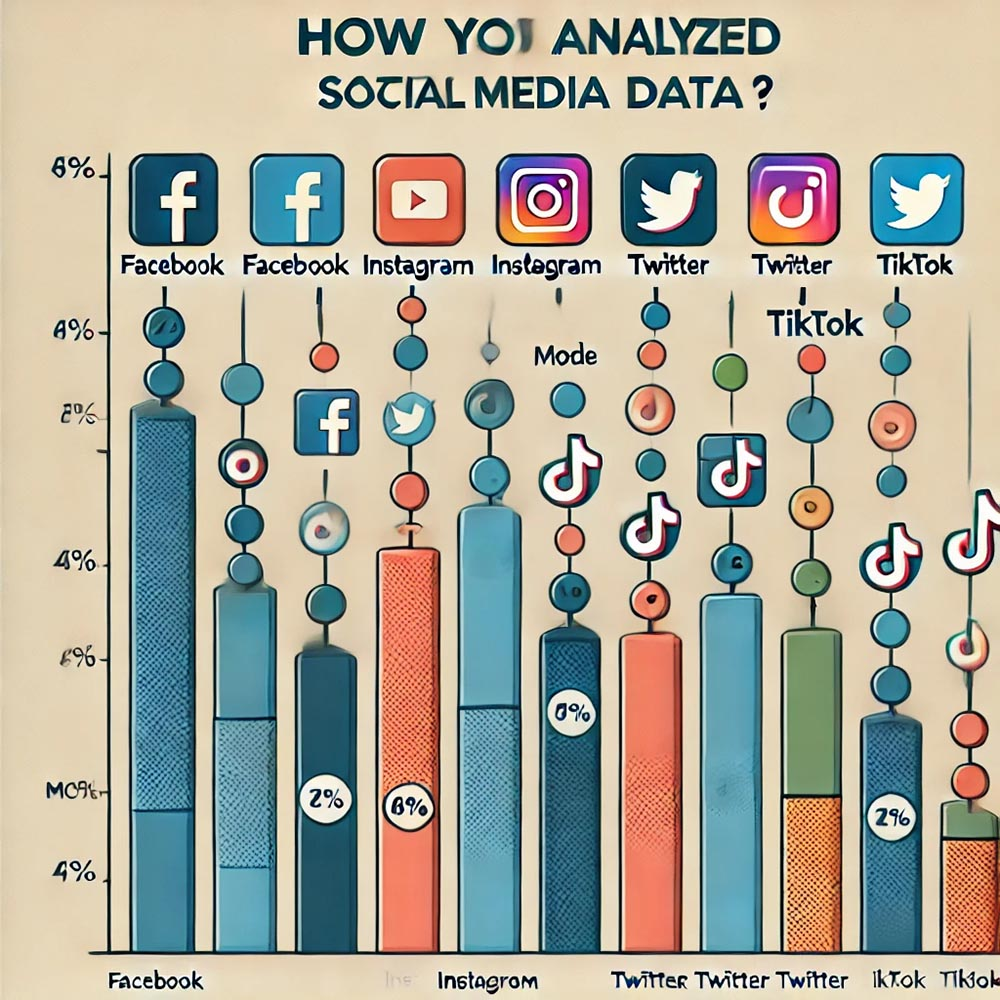
\includegraphics[width=1\textwidth,height=\textheight]{images/fig048.jpg}

\emph{Figure 048. A pie chart or bar chart showing the distribution of responses to a survey question about preferred social media platforms, with the mode (the most frequently chosen platform) clearly highlighted. This visual would help students understand how the mode is determined and why it is useful for analyzing categorical data.}

We will discuss the usefulness of the mode in understanding the most popular categories in a dataset, particularly in situations where you want to identify the most common value or category. You will engage in an activity where you identify the mode from various datasets, followed by a discussion on when it is appropriate to use the mode as a measure of central tendency.

Understanding the mean, median, and mode, and knowing when to use each measure, is crucial for accurately summarizing and interpreting data. Each measure offers a different perspective on the data, and choosing the right one depends on the characteristics of your data set and the specific research questions you are addressing. By mastering these measures of central tendency, you will be better equipped to analyze data in a way that accurately reflects the patterns and trends within your research.

\subsection{Measures of Dispersion}\label{measures-of-dispersion}

Measures of dispersion are statistical tools that provide insight into the spread or variability of data within a dataset. While measures of central tendency, such as the mean, median, and mode, offer information about the central point of the data, measures of dispersion help us understand how spread out the data points are around this central point. Understanding these measures---range, standard deviation, and variance---enables you to gain a fuller picture of your data, particularly in terms of how much variation exists within the dataset.

The \textbf{range} is the simplest measure of dispersion and is calculated as the difference between the highest and lowest values in a dataset. It provides a quick snapshot of the spread of the data. For example, if you were to survey a group of participants about their ages in a study on media consumption habits, and the youngest participant was 18 years old while the oldest was 60, the range would be 42 years. This tells you that there is a 42-year span between the youngest and oldest participants in your study.

The range is easy to calculate and gives a basic indication of variability. However, it has significant limitations, particularly its sensitivity to outliers---extremely high or low values that can skew the range. For instance, if most participants in the media consumption study are between 20 and 30 years old, but one participant is 60, the range would still be 42, which might not accurately reflect the overall age distribution of the group. Therefore, while the range can be informative, it should be used with caution and in conjunction with other measures of dispersion.

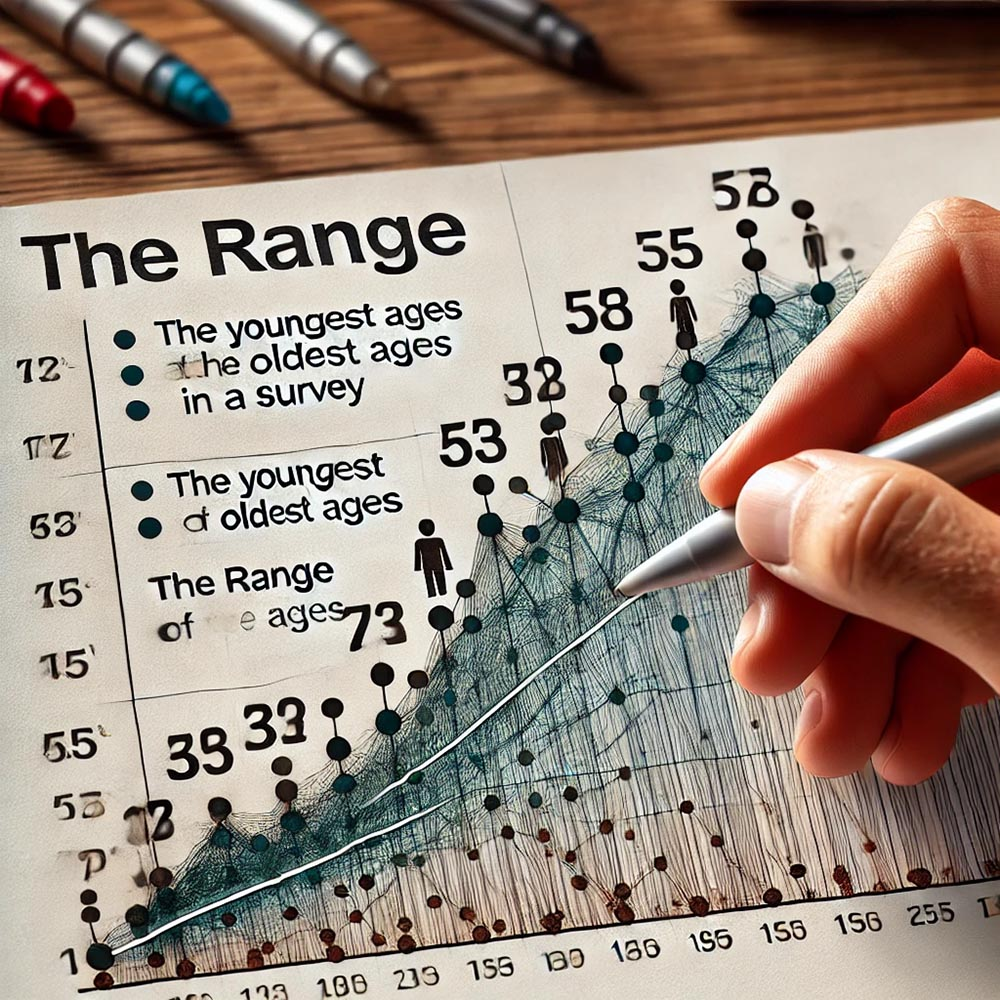
\includegraphics[width=1\textwidth,height=\textheight]{images/fig049.jpg}

\emph{Figure 049. A line graph or number line displaying the range of ages in a survey, with the youngest and oldest ages marked and the range highlighted. The visual could include an outlier to show how it affects the range. This image would help students visualize how the range is calculated and why it might not always be the best measure of dispersion when outliers are present.}

In our lessons, we will explore how the range provides a simple measure of variability. You will participate in an activity where you calculate the range for different datasets, including those with outliers, and discuss how these outliers can affect the range. This exercise will help you understand both the utility and the limitations of using range as a measure of dispersion.

The \textbf{standard deviation} is a more sophisticated measure of dispersion that indicates the amount of variation or spread in a set of values. Specifically, it tells you how much individual data points differ from the mean of the dataset. For example, if you were studying the daily time spent on social media among teenagers, calculating the standard deviation would help you understand whether most teenagers spend a similar amount of time on social media each day or whether there is a wide variation in their usage patterns.

The standard deviation is calculated by taking the square root of the variance (which we will discuss shortly). It provides a clear sense of the spread of the data around the mean: a low standard deviation indicates that the data points are close to the mean, while a high standard deviation suggests that the data points are spread out over a wider range of values. Understanding standard deviation is crucial because it allows you to assess the reliability and consistency of your data. In many research scenarios, particularly those involving large datasets, standard deviation is a key indicator of how much individual values deviate from the average.

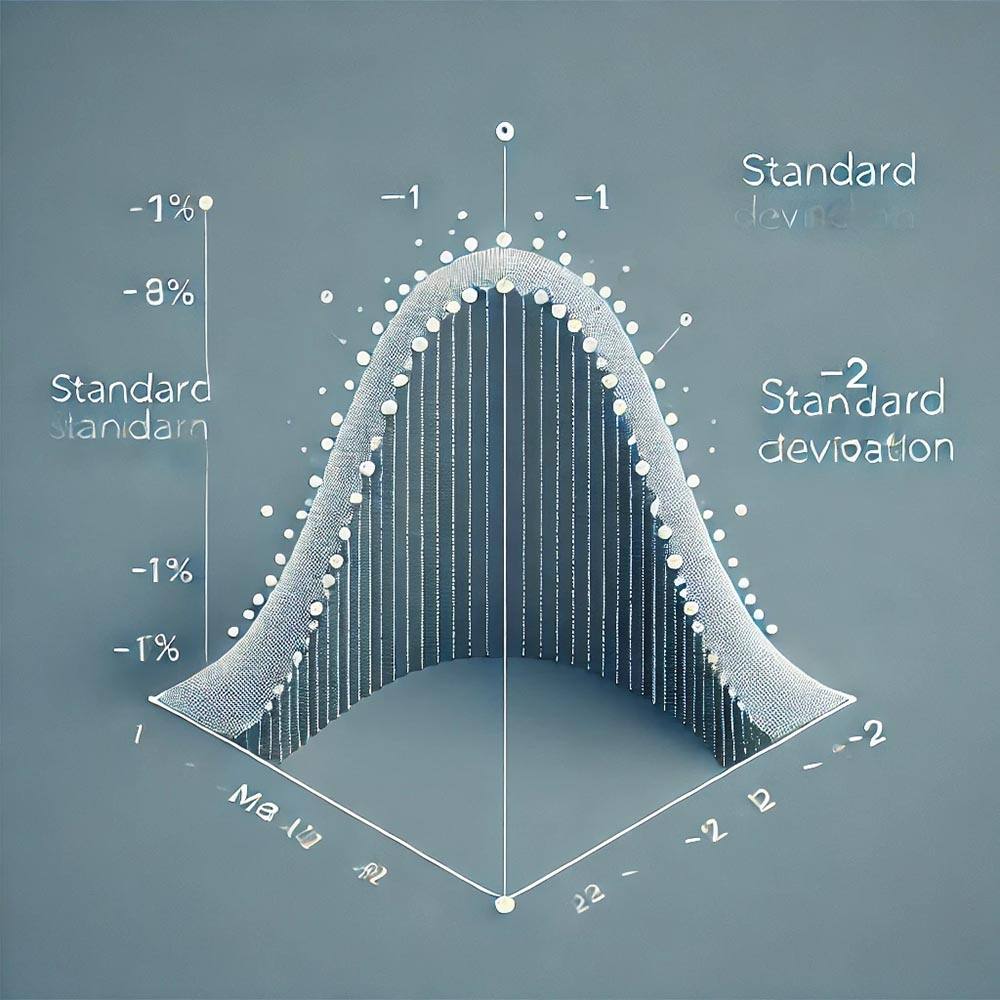
\includegraphics[width=1\textwidth,height=\textheight]{images/fig050.jpg}

\emph{Figure 050. A bell curve (normal distribution) with the mean marked in the center and standard deviations shown on either side of the mean (e.g., ±1, ±2 standard deviations). The visual could illustrate how data points are distributed around the mean and how standard deviation captures the spread of these data points. This image would help students grasp the concept of standard deviation and its significance in measuring data dispersion.}

To further your understanding, we will break down the formula for standard deviation and use visual aids to illustrate how it measures spread around the mean. You will be assigned an exercise where you calculate the standard deviation for a given dataset and interpret what it reveals about the dataset. This hands-on practice will deepen your understanding of standard deviation and its application in real-world research.

\textbf{Variance} is another important measure of dispersion, representing the average of the squared differences from the mean. Essentially, variance is the square of the standard deviation. While the standard deviation provides a measure of spread in the same units as the data itself, variance is expressed in squared units, making it less intuitive but very useful in statistical modeling and analysis.

Variance helps you understand the overall variability within your data and is particularly important in contexts where you need to compare the spread of different datasets or analyze data that is used in predictive models, such as regression analysis. For example, if you were examining the variance in viewer ratings for a TV show across different demographics, calculating the variance would give you insight into how consistent or varied these ratings are within each demographic group.

Although variance can sometimes seem abstract because it is expressed in squared units, it is fundamental to many statistical methods and models. It provides a foundation for understanding how data points are distributed and helps in making inferences about the broader population from which your sample is drawn.

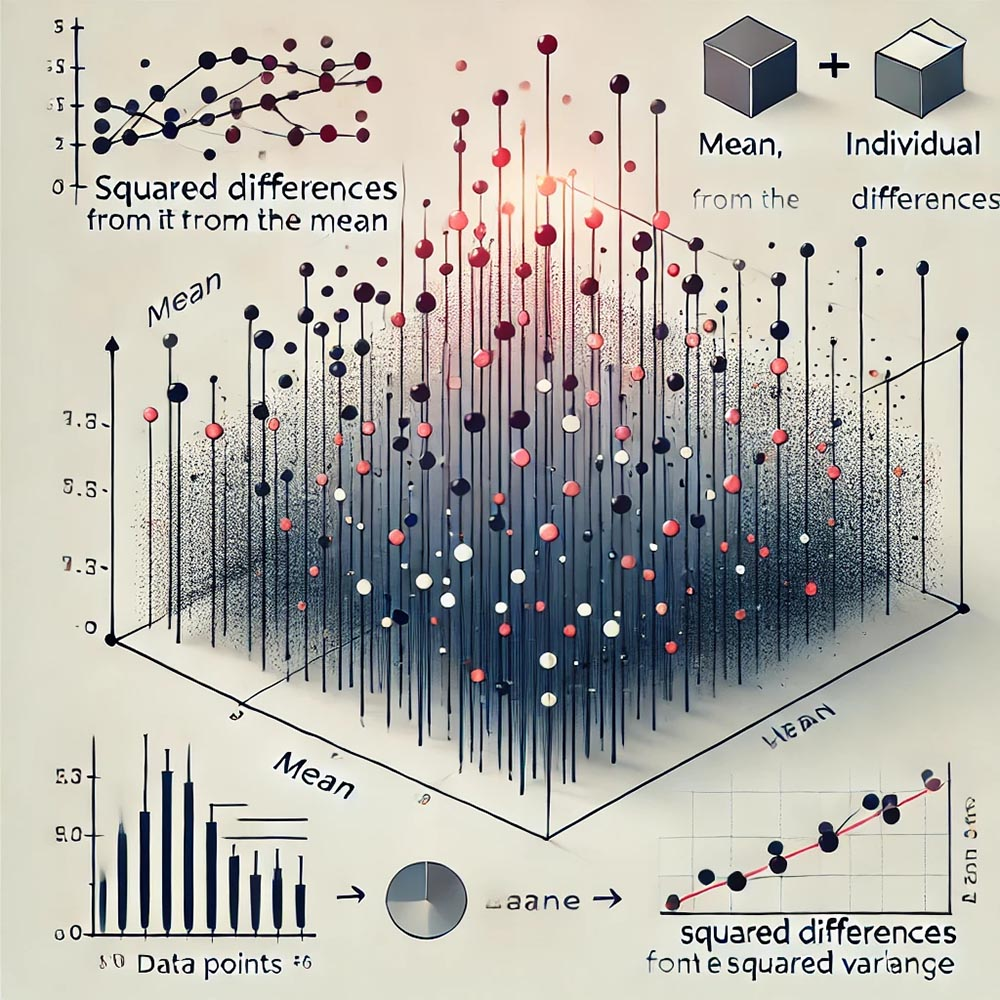
\includegraphics[width=1\textwidth,height=\textheight]{images/fig051.jpg}

\emph{Figure 051. A graphical representation of a dataset showing the mean, individual data points, and the squared differences from the mean. The visual could include the calculation steps for variance, illustrating how each squared difference contributes to the overall variance. This image would help students see how variance is calculated and why it is a crucial measure in statistical analysis.}

In our lessons, we will explore the relationship between variance and standard deviation and discuss why variance is often used in statistical models. You will calculate the variance for different datasets and compare it to the standard deviation to see how these measures of dispersion complement each other. This exercise will help you appreciate the role of variance in understanding data variability and its application in more advanced statistical analyses.

By mastering the concepts of range, standard deviation, and variance, you will be equipped to analyze the variability within your data, providing a more comprehensive understanding of your research findings. Each of these measures offers unique insights into the spread of data, and knowing when and how to use them is essential for conducting rigorous and meaningful research.

\section{Inferential Statistics}\label{inferential-statistics}

\subsection{Hypothesis Testing}\label{hypothesis-testing}

Hypothesis testing is a fundamental process in statistical analysis, allowing researchers to make inferences about a population based on sample data. The process involves making a hypothesis---a statement about a population parameter---and then using statistical methods to determine whether the data supports or contradicts this hypothesis. Understanding the components of hypothesis testing, such as p-values, Type I and Type II errors, and the distinction between one-tailed and two-tailed tests, is crucial for conducting rigorous and reliable research.

The \textbf{p-value} is a key concept in hypothesis testing. It represents the probability that the observed results are due to chance, assuming that the null hypothesis is true. In other words, the p-value helps you determine whether the evidence against the null hypothesis is strong enough to reject it. For example, if you were testing the difference in political views between two groups exposed to different news sources, the p-value would indicate the likelihood that any observed difference is simply due to random variation rather than a real effect of the news source on political views.

A low p-value (typically less than 0.05) suggests that the observed results are unlikely to have occurred by chance, leading researchers to reject the null hypothesis in favor of the alternative hypothesis. Conversely, a high p-value indicates that the data does not provide sufficient evidence to reject the null hypothesis, meaning any observed difference could be due to chance. Understanding p-values is crucial for interpreting the results of hypothesis tests accurately and making informed decisions about the validity of your research findings.

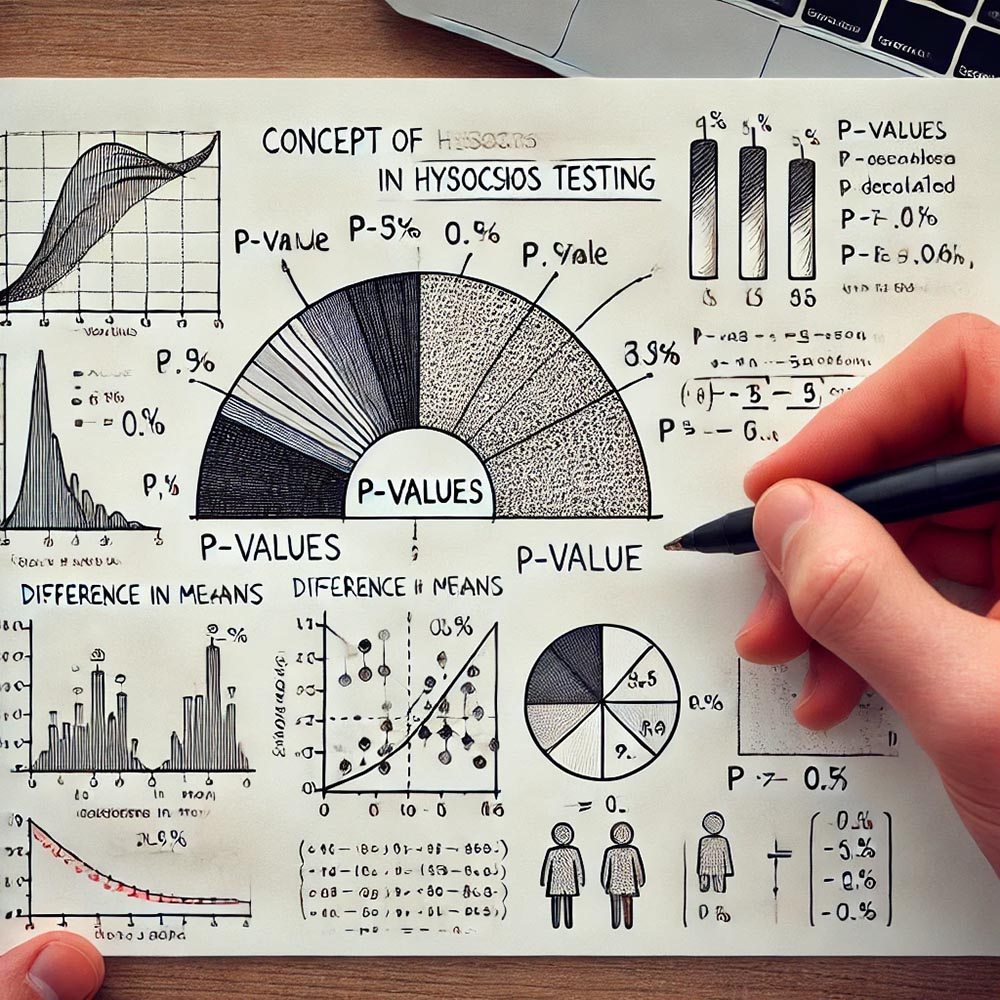
\includegraphics[width=1\textwidth,height=\textheight]{images/fig052.jpg}

\emph{Figure 052. A diagram illustrating the concept of p-values in hypothesis testing. The diagram could show a bell curve (normal distribution) with areas under the curve shaded to represent different p-value ranges (e.g., p \textless{} 0.05). The visual could also include an example scenario where p-values are calculated for a difference in means, helping students understand how p-values are derived and interpreted in the context of hypothesis testing.}

In our lessons, we will use real-life scenarios to explain what the p-value represents and how it is used in hypothesis testing. You will calculate p-values from sample data and interpret the results in the context of rejecting or failing to reject the null hypothesis. This hands-on approach will help you understand the role of p-values in making evidence-based decisions in research.

A \textbf{Type I error} occurs when a true null hypothesis is incorrectly rejected, also known as a false positive. This means that the researcher concludes there is an effect or difference when, in reality, there is none. For example, if a study concludes that a new social media feature increases user engagement when it actually does not, the researcher has made a Type I error. The consequences of Type I errors can be significant, leading to false conclusions and potentially misleading further research or practical applications based on those findings.

Minimizing Type I errors is important, especially in fields where false positives could lead to wasted resources or incorrect policy decisions. In hypothesis testing, the significance level (usually denoted as alpha, α) is set to control the likelihood of making a Type I error. A common alpha level is 0.05, meaning there is a 5\% chance of rejecting a true null hypothesis. However, this is a balance, as setting a very low alpha level to reduce Type I errors increases the risk of making Type II errors.

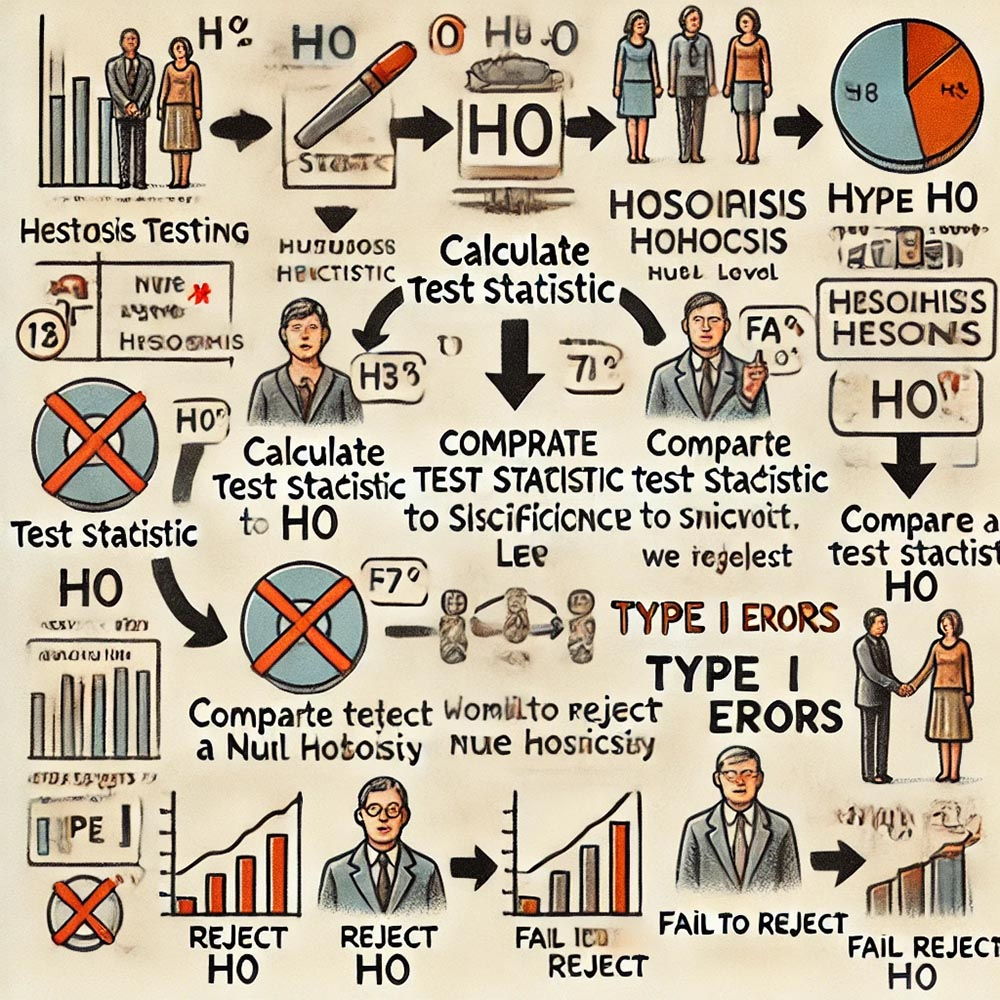
\includegraphics[width=1\textwidth,height=\textheight]{images/fig053.jpg}

\emph{Figure 053. A flowchart showing the decision-making process in hypothesis testing, highlighting where Type I errors occur. The chart could start with the null hypothesis, moving through the steps of calculating the test statistic and comparing it to the significance level, ending with either rejecting or failing to reject the null hypothesis. Annotations could point out the possibility of Type I errors when rejecting a true null hypothesis. This visual would help students understand how Type I errors arise and the importance of significance levels in controlling them.}

We will explore the consequences of Type I errors with examples from research and discuss strategies to minimize this error. You will engage in exercises where you identify potential Type I errors in hypothetical research scenarios, enhancing your ability to recognize and avoid these errors in your own research.

A \textbf{Type II error} occurs when a false null hypothesis is not rejected, also known as a false negative. This means that the researcher concludes there is no effect or difference when there actually is one. For example, if a study fails to detect that a change in advertising strategy actually improves sales, the researcher has made a Type II error. The implications of Type II errors can be equally significant, as they may lead to missed opportunities for effective interventions or incorrect assumptions that a treatment or strategy is ineffective.

The risk of Type II errors is related to the power of the statistical test, which is the probability of correctly rejecting a false null hypothesis. Factors such as sample size, effect size, and significance level all influence the power of a test. Researchers must balance the risk of Type I and Type II errors by choosing an appropriate significance level and ensuring their study is adequately powered to detect meaningful effects.

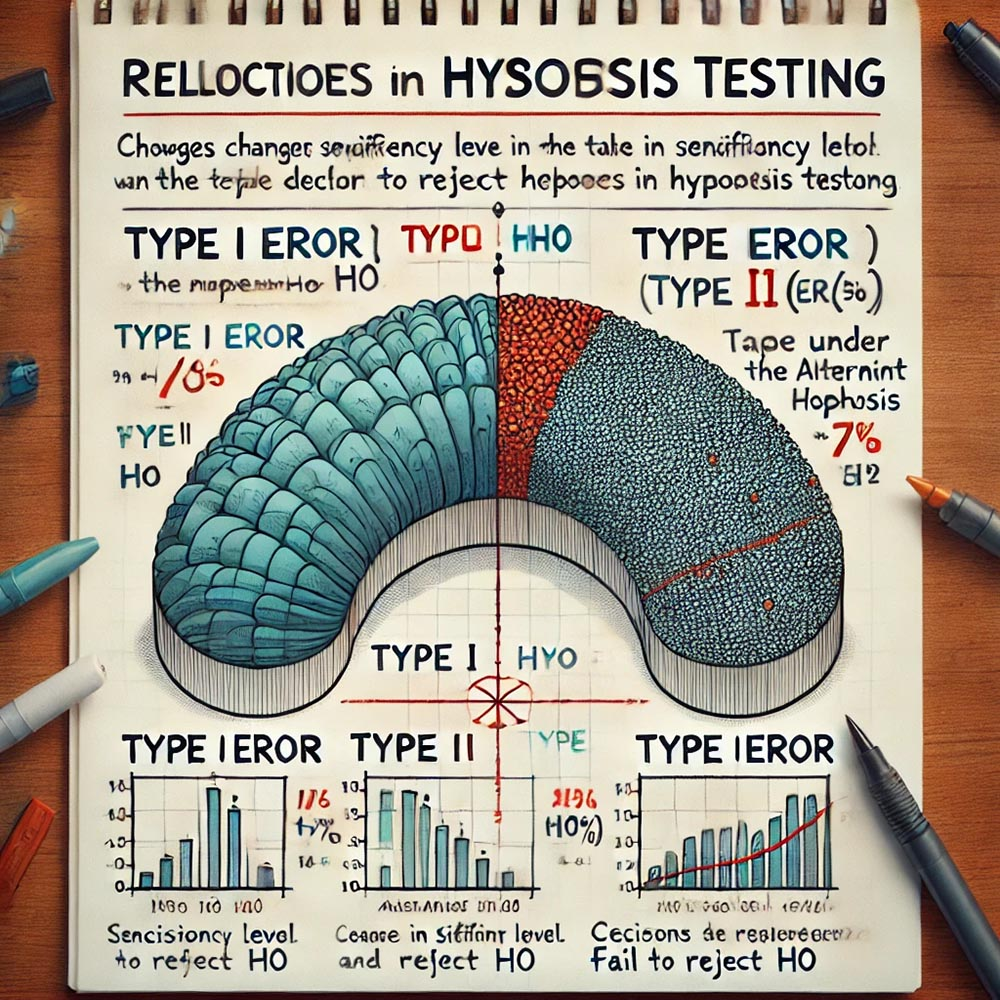
\includegraphics[width=1\textwidth,height=\textheight]{images/fig054.jpg}

\emph{Figure 054. A graph showing the relationship between Type I and Type II errors, with overlapping distributions representing the null and alternative hypotheses. The graph could include shaded areas to indicate where Type I and Type II errors occur, helping students visualize the trade-offs involved in hypothesis testing. This visual would aid in understanding how changes in significance level and sample size affect the likelihood of these errors.}

In class, we will discuss the trade-off between Type I and Type II errors and their implications in research. You will be assigned tasks where you calculate and interpret the potential for Type II errors in different experimental setups. This exercise will help you appreciate the importance of balancing these errors in your research design.

In hypothesis testing, the choice between a \textbf{one-tailed} and a \textbf{two-tailed} test depends on the nature of the research question. A one-tailed test is used when the research hypothesis specifies a direction of the effect (e.g., testing whether one group has a higher score than another). For example, if you are testing whether a new educational program increases test scores, you would use a one-tailed test because you are only interested in whether the program leads to higher scores, not lower scores.

A two-tailed test, on the other hand, is used when the research hypothesis does not specify a direction and simply tests for any difference, regardless of direction. For instance, if you are testing whether a new educational program affects test scores in any way (either increasing or decreasing them), a two-tailed test would be appropriate. The choice between one-tailed and two-tailed tests has implications for the significance level and the interpretation of results, as a one-tailed test focuses on one end of the distribution while a two-tailed test considers both ends.

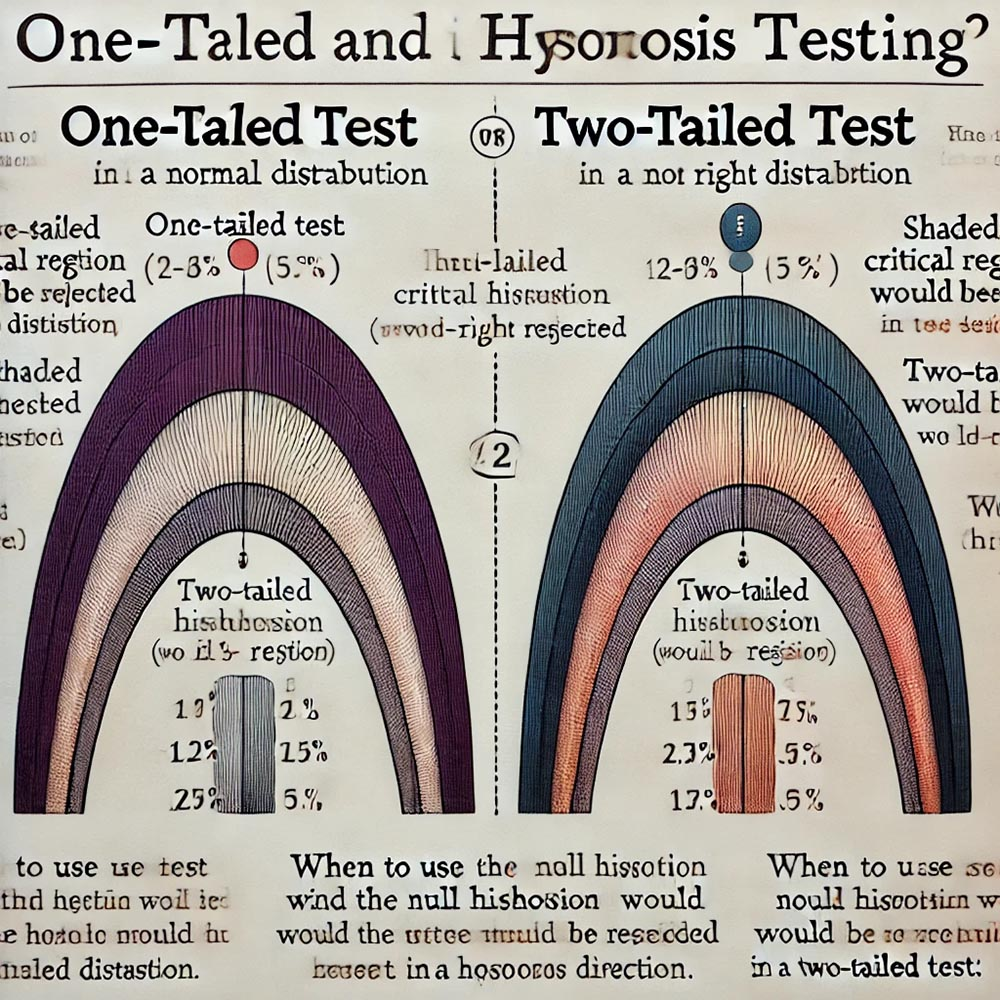
\includegraphics[width=1\textwidth,height=\textheight]{images/fig055.jpg}

\emph{Figure 055. A diagram comparing one-tailed and two-tailed tests, with bell curves showing the critical regions for each test. The one-tailed test could have a shaded area at one end of the distribution, while the two-tailed test could have shaded areas at both ends. This visual would help students understand the difference between the two types of tests and when to use each one based on their research question.}

We will use examples to illustrate when to use one-tailed versus two-tailed tests, and you will conduct an exercise where you choose between one-tailed and two-tailed tests based on specific research questions and justify your choice. This hands-on practice will help you develop the skills to select the appropriate test for your research and interpret the results accurately.

By mastering the concepts of p-values, Type I and Type II errors, and the distinction between one-tailed and two-tailed tests, you will be well-equipped to conduct hypothesis testing that is both rigorous and meaningful. These tools are essential for making informed decisions in research, allowing you to draw valid conclusions from your data and contribute to the advancement of knowledge in your field.

\subsection{Comparing Groups}\label{comparing-groups}

In research, comparing groups is a fundamental process that allows us to explore differences and draw meaningful conclusions about the relationships between variables. Various statistical tests are designed for this purpose, each suited to different types of data and research questions. Understanding how and when to use these tests---such as the t-test, ANOVA, Chi-Square Test, and ANCOVA---is essential for accurately interpreting data and making informed decisions based on research findings.

The \textbf{t-test} is one of the most commonly used statistical tests, particularly when the goal is to compare the means of two groups to determine if they are significantly different from each other. This test is especially useful in situations where you want to see if there is a difference between two distinct groups on some continuous outcome. For instance, if you are comparing the average time spent on social media between males and females, the t-test can help you determine whether the observed difference in means is statistically significant or if it might have occurred by chance.

The t-test operates by calculating the difference between the group means and determining whether this difference is large enough to be considered statistically significant, given the variability in the data and the sample sizes. The result is a t-statistic, which is then compared to a critical value from the t-distribution to determine the significance of the result.

\includegraphics[width=1\textwidth,height=\textheight]{images/fig056.jpg}

\emph{Figure 056. A graph showing the distributions of two groups (e.g., males and females) with their respective means marked, alongside the calculation of the t-statistic. The image could include a depiction of the overlap between the two distributions, helping students visualize how the t-test assesses whether the means are significantly different. This visual would aid in understanding the concept of the t-test and its application to comparing group means.}

In our lessons, we will explain the concept of the t-test with concrete examples and walk you through the calculation process step by step. You will have the opportunity to perform t-tests using sample data, interpret the results, and discuss potential sources of error, such as unequal variances or small sample sizes, that could affect the reliability of your conclusions.

When research involves comparing the means of three or more groups, the \textbf{Analysis of Variance (ANOVA)} becomes the appropriate statistical test. ANOVA extends the logic of the t-test to multiple groups, allowing you to determine whether at least one group mean is different from the others. For example, if you were interested in comparing average TV viewing times across different age groups---say, teenagers, adults, and seniors---ANOVA would help you assess whether the observed differences in viewing times are statistically significant.

The ANOVA process involves calculating the variance within each group and the variance between groups to produce an F-ratio. This ratio is then compared to a critical value from the F-distribution to determine whether the group means differ significantly. If the ANOVA indicates significant differences, post-hoc tests are often conducted to pinpoint which specific groups differ from each other.

\includegraphics[width=1\textwidth,height=\textheight]{images/fig057.jpg}

\emph{Figure 057. A diagram showing the concept of variance within groups and between groups, leading to the calculation of the F-ratio. The visual could include a simple example with three groups and their means, illustrating how ANOVA partitions the total variance to assess group differences. This image would help students grasp the concept of ANOVA and its application to comparing multiple group means.}

We will break down the ANOVA process, explaining how it extends the t-test to more than two groups. You will conduct an ANOVA on a dataset and discuss the interpretation of F-ratios and the results of post-hoc tests, which are critical for identifying specific group differences after finding a significant overall effect.

The \textbf{Chi-Square Test} is another valuable statistical tool, particularly when dealing with categorical data. This test is used to examine the association between categorical variables, helping researchers understand whether the distribution of one variable differs significantly across the levels of another variable. For instance, if you wanted to analyze the relationship between gender and preferred news source, the Chi-Square Test would allow you to determine whether the distribution of news source preferences differs significantly between males and females.

The Chi-Square Test works by comparing the observed frequencies of each category combination with the frequencies that would be expected if there were no association between the variables. The result is a chi-square statistic, which is then compared to a critical value from the chi-square distribution to assess the significance of the association.

\includegraphics[width=1\textwidth,height=\textheight]{images/fig058.jpg}

\emph{Figure 058. A contingency table showing the observed frequencies of gender by preferred news source, alongside the expected frequencies if there were no association. The visual could include the calculation of the chi-square statistic, helping students understand how the test compares observed and expected frequencies. This image would help clarify how the Chi-Square Test assesses associations between categorical variables.}

We will explain the Chi-Square Test using contingency tables and real-life examples, helping you understand how to conduct and interpret the test in your own research. You will practice conducting chi-square tests and interpreting the results, focusing on the implications of significant associations for your research questions.

Finally, the \textbf{Analysis of Covariance (ANCOVA)} combines the principles of ANOVA with regression to compare group means while adjusting for the effects of covariates. This makes ANCOVA particularly useful when you need to control for potential confounding variables that might influence the outcome of interest. For example, if you were comparing the effectiveness of different advertising strategies across various media while controlling for viewer income levels, ANCOVA would allow you to adjust the group means for income differences before making comparisons.

ANCOVA operates by first using regression to remove the influence of the covariate on the dependent variable, then performing an ANOVA on the adjusted means. This allows for a more accurate comparison of group effects, accounting for the variance explained by the covariate.

\includegraphics[width=1\textwidth,height=\textheight]{images/fig059.jpg}

\emph{Figure 059. A diagram illustrating the steps of ANCOVA, showing how the covariate is used to adjust group means before conducting ANOVA. The visual could include a simple example with a covariate (e.g., income) and its effect on the outcome (e.g., advertising effectiveness), helping students understand the process of adjusting for covariates in group comparisons. This image would aid in understanding how ANCOVA controls for confounding variables and allows for more accurate group comparisons.}

We will introduce ANCOVA by discussing how it adjusts for potential confounding variables and when it is appropriate to use this test. You will analyze a dataset using ANCOVA and interpret the adjusted group means, deepening your understanding of how to control for confounds in research.

By mastering these statistical tests---t-test, ANOVA, Chi-Square Test, and ANCOVA---you will be well-equipped to compare groups in your research and draw valid, meaningful conclusions. Each test serves a specific purpose and is essential for analyzing different types of data, allowing you to explore relationships and differences with precision and confidence.

\subsection{Correlation and Regression}\label{correlation-and-regression}

Understanding the relationship between variables is central to conducting research and making informed predictions. Two key statistical tools used for this purpose are correlation and regression. These methods allow researchers to explore and quantify the relationships between variables, assess the strength and direction of these relationships, and make predictions based on observed data.

\textbf{Correlation} is a statistical measure that describes the strength and direction of a relationship between two variables. It helps you understand whether and how strongly pairs of variables are related. The most commonly used correlation measure is \textbf{Pearson's r}, which ranges from -1 to 1. A Pearson's r value of 1 indicates a perfect positive linear relationship, meaning that as one variable increases, the other also increases proportionally. A value of -1 indicates a perfect negative linear relationship, where an increase in one variable corresponds to a decrease in the other. A value of 0, on the other hand, indicates no linear relationship between the variables.

For instance, if you wanted to examine the relationship between time spent on social media and self-reported stress levels, you might calculate the Pearson's r correlation coefficient. A positive correlation would suggest that as time on social media increases, stress levels also increase, while a negative correlation would indicate the opposite. No significant correlation would imply that time on social media and stress levels are not linearly related.

\includegraphics[width=1\textwidth,height=\textheight]{images/fig060.jpg}

\emph{Figure 060. A scatter plot showing the relationship between two variables, such as time spent on social media and stress levels, with a line of best fit indicating the direction of the correlation. The plot could include examples of different correlation strengths (e.g., strong positive, strong negative, and no correlation) to help students visually understand what Pearson's r values represent. This image would clarify how correlation coefficients reflect the strength and direction of relationships between variables.}

In our lessons, we will use scatter plots to visually explain correlation and introduce Pearson's r. You will calculate correlation coefficients for different datasets and discuss what the values indicate about the relationships. This hands-on practice will help you understand how correlation is used to explore relationships between variables and the limitations of this method, such as its inability to imply causation.

\textbf{Regression} is another powerful statistical tool used to predict the value of a dependent variable based on one or more independent variables. While correlation measures the strength and direction of a relationship, regression goes further by modeling this relationship mathematically. \textbf{Linear regression} is the simplest form of regression, where the relationship between the dependent and independent variables is modeled as a straight line (y = mx + b). The coefficients in this equation (m and b) represent the slope of the line and the y-intercept, respectively, providing insights into how changes in the independent variable(s) affect the dependent variable.

For example, if you wanted to predict the likelihood of someone sharing news articles based on their social media habits, you might use logistic regression, which is a form of regression used when the dependent variable is binary (e.g., yes/no, success/failure). Logistic regression would allow you to model the probability that a given individual will share news articles based on factors like time spent on social media, frequency of news consumption, and other relevant variables.

\includegraphics[width=1\textwidth,height=\textheight]{images/fig061.jpg}

\emph{Figure 061. A diagram illustrating the concept of linear regression, showing a scatter plot with a regression line (line of best fit) and the equation of the line. The visual could also include examples of how changing the slope and intercept affects the predictions. This image would help students understand the basics of linear regression and how it is used to make predictions based on data.}

In class, we will explain the basics of linear regression, including the interpretation of coefficients and how these coefficients reflect the relationship between variables. You will conduct simple and multiple regression analyses and interpret the results in terms of prediction and variance explained. This will give you a strong foundation in using regression analysis to make informed predictions in your research.

An important concept related to regression is \textbf{regression toward the mean}. This phenomenon occurs when an extreme value on one measurement tends to be closer to the average on a subsequent measurement. For example, students who score very high or very low on an initial test are likely to score closer to the mean on a retest. This can happen due to the natural variability in data and the influence of random factors that are less likely to recur on a second measurement.

Understanding regression toward the mean is crucial because it can affect the interpretation of research findings, especially in longitudinal studies where the same individuals are measured multiple times. If not accounted for, this phenomenon can lead researchers to incorrectly attribute changes to an intervention or treatment when they are simply due to natural variability.

\includegraphics[width=1\textwidth,height=\textheight]{images/fig062.jpg}

\emph{Figure 062. A graph showing a set of initial scores and subsequent scores, with a regression line indicating the movement of extreme scores toward the mean on the retest. The visual could highlight how scores that were initially high or low tend to be closer to the average on the second measurement. This image would help students visualize the concept of regression toward the mean and understand its implications in research.}

We will discuss regression toward the mean with visual examples, such as tracking performance over time, to help you recognize this phenomenon in your research. You will engage in identifying scenarios where regression toward the mean might affect research findings and learn strategies to account for it in your analyses.

By mastering the concepts of correlation, regression, and regression toward the mean, you will be well-equipped to explore relationships between variables, make accurate predictions, and avoid common pitfalls in data analysis. These tools are essential for conducting robust and insightful research, allowing you to draw meaningful conclusions from your data.

\section{Advanced Statistical Techniques}\label{advanced-statistical-techniques}

\subsection{Multivariate Analysis}\label{multivariate-analysis}

In research, particularly when dealing with complex datasets, it's often necessary to analyze multiple dependent variables simultaneously or to simplify large sets of variables into more manageable components. This is where multivariate analysis techniques like MANOVA (Multivariate Analysis of Variance) and factor analysis become invaluable. These methods allow researchers to gain deeper insights into their data by examining relationships between multiple variables and by reducing the dimensionality of complex data sets.

\textbf{MANOVA}, or Multivariate Analysis of Variance, is an extension of the ANOVA technique. While ANOVA compares means across groups for a single dependent variable, MANOVA allows researchers to compare means across multiple dependent variables simultaneously. This method is particularly useful when you are interested in understanding how different groups differ across several related outcomes. For instance, if you wanted to examine how different media consumption habits affect both political knowledge and civic engagement, MANOVA would enable you to analyze these two outcomes together rather than separately.

One of the key advantages of MANOVA over conducting multiple ANOVAs is that it accounts for the potential correlations between dependent variables. This reduces the likelihood of committing a Type I error (false positive) that can occur when multiple tests are run independently. By considering the combined variance in the dependent variables, MANOVA provides a more comprehensive understanding of group differences.

\includegraphics[width=1\textwidth,height=\textheight]{images/fig063.jpg}

\emph{Figure 063. A flowchart illustrating the MANOVA process, starting with the identification of multiple dependent variables and moving through to the comparison of means across groups. The chart could also highlight how MANOVA handles correlations between dependent variables, offering a visual explanation of why this method is preferred over multiple independent ANOVAs. This image would help students grasp the concept of MANOVA and understand its application in research.}

In our lessons, we will introduce MANOVA by explaining its advantages over multiple ANOVAs. You will conduct a MANOVA on a dataset and interpret the multivariate test results, focusing on what these results mean for your research findings. This hands-on experience will help you appreciate the power of MANOVA in analyzing complex data and making nuanced comparisons across multiple outcomes.

\textbf{Factor analysis} is another powerful tool used in multivariate analysis. This technique is designed to reduce a large number of variables into a smaller set of underlying factors. These factors represent the shared variance among the variables, effectively identifying patterns or dimensions within the data. For example, if you conducted a survey with multiple questions aimed at measuring audience engagement, factor analysis could help you identify key dimensions of engagement, such as attention, interaction, and satisfaction, by grouping related questions together.

There are two main types of factor analysis: exploratory and confirmatory. \textbf{Exploratory factor analysis (EFA)} is used when you want to uncover the underlying structure of your data without prior hypotheses about how the variables are related. It is a data-driven approach that helps you identify possible factors that explain the observed correlations among variables. \textbf{Confirmatory factor analysis (CFA)}, on the other hand, is used when you have specific hypotheses about the factor structure and want to test how well your data fits this predefined model.

\includegraphics[width=1\textwidth,height=\textheight]{images/fig064.jpg}

\emph{Figure 064. A diagram showing the process of factor analysis, from the initial data with many variables to the extraction of a few key factors. The visual could include a matrix of variable correlations and the resulting factors that group related variables together. This image would help students understand how factor analysis simplifies complex data by identifying underlying relationships between variables.}

We will explain the concepts of exploratory and confirmatory factor analysis using visual aids to show how factors are extracted from a dataset. You will perform a factor analysis on a dataset, interpreting the resulting factors and discussing how these can be used to simplify complex data. This exercise will provide you with practical experience in reducing data complexity and uncovering the hidden structure within your data.

By mastering MANOVA and factor analysis, you will gain the ability to handle complex datasets with multiple dependent variables or large numbers of variables that need to be distilled into core dimensions. These multivariate analysis techniques are essential for conducting sophisticated research that can reveal deeper insights and more nuanced understandings of the phenomena you study.

\section{Controlling for Confounds}\label{controlling-for-confounds}

When conducting research, one of the most critical tasks is ensuring that the relationships you observe between variables are valid and not influenced by other, unaccounted-for factors. These unaccounted-for factors, known as confounds, can lead to incorrect conclusions if not properly managed. Understanding how to identify and control for confounds is essential for any researcher aiming to produce accurate and reliable results.

\textbf{Confounds} are variables that might influence the dependent variable in your study but are not the primary focus of your research. For instance, if you are studying the effect of media exposure on anxiety levels, a potential confound could be the participants' baseline anxiety levels before the media exposure. If these baseline levels vary significantly across participants and are not accounted for, they could skew your results, leading you to incorrectly attribute changes in anxiety to media exposure rather than to the pre-existing differences in anxiety.

To illustrate how confounds can distort research findings, consider a hypothetical study where you measure anxiety levels before and after participants watch a news broadcast. If some participants have high baseline anxiety levels due to unrelated factors (such as personal stressors), these levels could increase after watching the broadcast, not necessarily because of the broadcast itself but because of their pre-existing condition. If you don't account for this confound, you might wrongly conclude that the news broadcast has a greater effect on anxiety than it actually does.

\includegraphics[width=1\textwidth,height=\textheight]{images/fig065.jpg}

\emph{Figure 065. A flowchart depicting the research process with and without controlling for confounds. The flowchart could show a simple research design where a confound influences the dependent variable, leading to incorrect conclusions, alongside a design where the confound is identified and controlled, resulting in a more accurate interpretation of the results. This visual would help students understand the importance of identifying and managing confounds in their research.}

To address this issue, researchers use various strategies to identify potential confounds during the study design phase and apply methods to control for them during analysis. For example, in the design phase, you might use random assignment to ensure that potential confounds are evenly distributed across experimental groups. Alternatively, during the analysis phase, you can apply \textbf{statistical control} techniques to hold constant the effects of confounding variables while examining the relationship between your independent and dependent variables.

\textbf{Statistical control} involves using techniques like ANCOVA (Analysis of Covariance) or regression to adjust for the influence of confounding variables. For instance, if you are comparing media consumption habits across different income groups but suspect that age might be a confounding factor, you could use ANCOVA to control for age. This technique would adjust the group means for age differences before comparing them, allowing you to isolate the effect of income on media consumption more accurately.

By controlling for confounds, you reduce the likelihood that your results are influenced by extraneous variables, thereby increasing the internal validity of your study. This process is critical in ensuring that the relationships you observe truly reflect the influence of the independent variable on the dependent variable rather than the impact of confounding factors.

\includegraphics[width=1\textwidth,height=\textheight]{images/fig066.jpg}

\emph{Figure 066. A diagram showing the process of statistical control using ANCOVA, with an example dataset where age is controlled while comparing media consumption across income groups. The diagram could include before-and-after visuals, showing the comparison of group means without control and with ANCOVA applied. This image would help students understand how statistical control works and why it's important in research.}

In our lessons, we will discuss the concept of statistical control and how it can be implemented using methods like ANCOVA or regression. You will be assigned to design a study where you apply statistical control techniques and interpret the adjusted results. This hands-on experience will help you appreciate the importance of controlling for confounds in producing accurate and reliable research findings.

Another important concept to understand when analyzing the effects of variables is \textbf{interaction}. An interaction occurs when the effect of one independent variable on the dependent variable differs depending on the level of another independent variable. For example, consider a study examining how media literacy training affects the ability to identify fake news. The effect of the training might differ based on the participants' education level; in other words, the effectiveness of the training could be greater for those with higher education levels compared to those with lower education levels. This is an example of an interaction effect, where the impact of media literacy training is not uniform across all participants but varies depending on another factor (education level).

Understanding interactions is crucial because they reveal the complexity of relationships between variables. Without considering interaction effects, you might miss important nuances in your data and draw incomplete or misleading conclusions.

\includegraphics[width=1\textwidth,height=\textheight]{images/fig067.jpg}

\emph{Figure 067. A graph showing an interaction effect, with two lines representing the impact of media literacy training on identifying fake news at different education levels. The graph could show how the lines diverge, indicating that the effect of the training varies depending on education. This visual would help students grasp the concept of interaction effects and how they reveal complex relationships between variables.}

We will use examples to demonstrate how interactions are tested and interpreted in statistical analyses. You will engage in performing interaction analyses using regression or ANOVA, and discuss the implications of significant interactions in your research findings. This exercise will deepen your understanding of how variables interact in complex ways and how to account for these interactions in your analyses.

By mastering the concepts of confounds, statistical control, and interaction, you will be better equipped to design rigorous studies and analyze data in a way that yields accurate and meaningful results. These skills are essential for any researcher committed to producing high-quality research that can withstand critical scrutiny.

\chapter{Data Management and Visualization}\label{data-management-and-visualization}

\section{RStudio}\label{rstudio}

\subsection{Introduction to RStudio}\label{introduction-to-rstudio}

RStudio is an integrated development environment (IDE) that makes working with the R programming language more user-friendly, providing a powerful platform for statistical computing and data analysis. Understanding how to code in R, import and export data, and handle errors effectively are fundamental skills that will enhance your ability to conduct sophisticated data analyses and produce reliable research findings.

\textbf{Coding in R} is the first step toward unlocking the full potential of this powerful tool. R is a programming language designed specifically for data manipulation, statistical analysis, and graphical representation. To get started, it's essential to familiarize yourself with the basics of R syntax. This includes understanding how to assign variables, recognize different data types (such as numeric, character, and factor), and perform basic operations like arithmetic calculations and logical comparisons.

For example, you might write a simple R script to calculate summary statistics for a dataset. This script could include commands to calculate the mean, median, and standard deviation of a numeric variable. By learning how to write such scripts, you will be able to automate repetitive tasks and perform complex analyses with ease.

\includegraphics[width=1\textwidth,height=\textheight]{images/fig068.jpg}

\emph{Figure 068. A screenshot of the RStudio interface with a basic R script visible in the script editor. The script might include simple commands for variable assignment, basic arithmetic operations, and the calculation of summary statistics. This image would help students visualize the coding environment and understand where to write and execute their code in RStudio.}

We will begin with the basics of R syntax, starting with variable assignment and data types, and then move on to basic operations. Hands-on exercises will allow you to write and execute simple R scripts in RStudio, helping you become comfortable with the coding environment. To support your learning, you will have access to resources like R cheat sheets or coding snippets for common tasks. These resources will be invaluable as you build your coding confidence and begin to tackle more complex analyses.

Once you are comfortable with basic coding, it's crucial to learn how to \textbf{import and export data} in RStudio. In research, data often comes in various formats, such as CSV files, Excel spreadsheets, or even databases. RStudio allows you to import data from these sources using functions like \texttt{read.csv()} for CSV files or \texttt{read\_excel()} for Excel files. Similarly, once you've completed your analysis, you may need to export your results for further use, which can be done with functions like \texttt{write.csv()}.

For instance, you might import a CSV file containing survey data into RStudio for analysis. After performing basic data manipulations, such as cleaning up missing values or transforming variables, you would then export the cleaned dataset to share with colleagues or use in further analyses.

\includegraphics[width=1\textwidth,height=\textheight]{images/fig069.jpg}

\emph{Figure 069. A flowchart showing the steps to import data into RStudio, perform data manipulation, and then export the results. The chart could include visual cues like CSV file icons, RStudio interface elements, and a final output file. This image would help students understand the workflow of data handling in RStudio, from import to export.}

We will demonstrate how to use the \texttt{read.csv()} function to import data and the \texttt{write.csv()} function to export results. You will be assigned an activity where you import a dataset, perform basic data manipulation, and then export the cleaned dataset. During this process, we will discuss common issues that arise during data import/export, such as dealing with missing values or formatting inconsistencies, and how to resolve them effectively.

Another important skill to develop when working with RStudio is \textbf{error handling}. In coding, errors are inevitable, but learning how to identify, diagnose, and correct them is a critical part of becoming proficient in R. Errors in R can range from syntax errors (e.g., forgetting a parenthesis) to logical errors (e.g., using the wrong formula for a calculation). Understanding how to interpret error messages and debug your code will save you time and frustration.

For example, you might encounter an error in your script due to incorrect data types---such as trying to perform arithmetic operations on character data. Debugging this issue would involve checking the data type of the variable and converting it to a numeric type if necessary.

\includegraphics[width=1\textwidth,height=\textheight]{images/fig070.jpg}

\emph{Figure 070. A screenshot of RStudio displaying an error message in the console, with the corresponding line of code highlighted in the script editor. The image could also include annotations explaining the error and the steps needed to correct it. This visual would help students understand how to troubleshoot errors and learn from the error messages provided by R.}

We will introduce you to common types of errors in R, such as syntax and logical errors, and teach you how to interpret the error messages generated by RStudio. You will engage in troubleshooting exercises where you debug pre-written scripts that contain intentional errors. These exercises will help you develop the skills needed to diagnose and fix issues in your own code. We will also discuss best practices for writing error-free code, such as using comments to document your code, keeping your code modular (breaking it down into small, manageable sections), and testing small sections of code before running larger scripts.

By mastering these fundamental aspects of using RStudio---coding in R, importing and exporting data, and handling errors---you will be well-equipped to perform sophisticated data analyses and contribute to high-quality research. These skills will serve as the foundation for more advanced topics in data science and statistical analysis, empowering you to explore and analyze data with confidence and precision.

\subsection{Data Management in R}\label{data-management-in-r}

Effective data management is crucial for ensuring the integrity and reliability of your analysis in R. Whether you are dealing with large datasets or small ones, the principles of data accuracy, coding of data, and understanding dataset variability are essential components of the research process. This section will guide you through the fundamental steps of managing data in R, helping you to ensure that your analyses are based on accurate, well-organized, and appropriately coded data.

\textbf{Data Accuracy} is the cornerstone of any reliable analysis. Before you can perform any meaningful statistical tests or draw conclusions from your data, you must ensure that the data itself is accurate and free from errors. This involves thoroughly checking the dataset for issues such as incorrect data entries, missing values, and outliers that could skew your results. For example, if you are working with survey responses, you might encounter data entry errors where a respondent's age is listed as ``150'' instead of ``15.'' Identifying and correcting such errors is essential to maintain the integrity of your analysis.

To assist in this process, R provides several functions that allow you to inspect and clean your dataset. The \texttt{summary()} function, for example, provides a quick overview of the dataset, showing the minimum, maximum, mean, and other statistics for each variable. Similarly, the \texttt{str()} function offers a detailed look at the structure of the dataset, including the type and class of each variable. By using these tools, you can identify potential inaccuracies in your data and take steps to correct them before proceeding with your analysis.

\includegraphics[width=1\textwidth,height=\textheight]{images/fig071.jpg}

\emph{Figure 071. A screenshot of RStudio showing the output of the \texttt{summary()} and \texttt{str()} functions applied to a sample dataset. The image could highlight areas where data anomalies (such as outliers or missing values) are visible, with annotations explaining how these might affect analysis if not addressed. This visual would help students understand how to use these functions to assess and ensure data accuracy.}

We will start by teaching you how to use functions like \texttt{summary()} and \texttt{str()} to inspect datasets for accuracy. You will then be assigned tasks where you clean and verify the accuracy of a dataset by identifying and correcting errors such as duplicates, outliers, or missing values. This hands-on practice will help you develop the skills needed to maintain data accuracy in your own research.

After ensuring that your data is accurate, the next step is the \textbf{Coding of Data}. Coding involves categorizing and assigning numerical or categorical labels to your data, which is particularly important when dealing with qualitative data that needs to be converted into a format suitable for quantitative analysis. For instance, if your dataset includes open-ended survey responses where participants expressed their level of agreement with a statement, you might code these responses as numerical values (e.g., 1 = ``Agree'', 2 = ``Disagree'').

Accurate coding is essential because it directly affects the outcomes of your statistical analyses. Inconsistent or incorrect coding can lead to misleading results, so it's important to approach this task with care. Consistency is key: each category should be clearly defined, and all data points should be coded according to these definitions. This ensures that your analyses are based on standardized data, which in turn leads to more reliable conclusions.

\includegraphics[width=1\textwidth,height=\textheight]{images/fig072.jpg}

\emph{Figure 072. A table showing a small dataset of qualitative survey responses before and after coding. The image could include annotations that explain the coding process and highlight the importance of consistency in coding, such as ensuring all ``Agree'' responses are coded as ``1'' across the entire dataset. This visual would help students understand the practical aspects of coding qualitative data for quantitative analysis.}

We will provide examples of how to code qualitative data for quantitative analysis, and you will practice coding data by categorizing and labeling a small dataset. This exercise will be followed by a discussion on the importance of consistency and accuracy in coding, ensuring that you understand the impact of these practices on your overall research.

Finally, understanding \textbf{Dataset Variability} is crucial for interpreting your data and making informed conclusions. Variability refers to the spread or dispersion of data points within a dataset, and it provides insights into the consistency and reliability of the data. For example, if you are analyzing test scores among students from different schools, variability can tell you how much the scores differ within and between schools. High variability might indicate significant differences in performance, while low variability could suggest more uniform outcomes.

In R, variability can be measured using statistics like variance and standard deviation, which quantify the extent to which data points deviate from the mean. Additionally, visual tools like boxplots or histograms can help you to visualize variability, making it easier to interpret the data and identify any patterns or anomalies.

\includegraphics[width=1\textwidth,height=\textheight]{images/fig073.jpg}

\emph{Figure 073. A side-by-side comparison of a boxplot and a histogram of a dataset in RStudio, showing the distribution of data points and highlighting the variability. The image could include annotations explaining how to interpret the spread of the data and what it suggests about the dataset's reliability. This visual would help students grasp the concept of variability and how to measure and interpret it using statistical and visual tools.}

We will explain the concept of variability and how it can be measured using statistics like variance and standard deviation. You will use visual tools like boxplots or histograms to help understand and interpret variability in datasets. Through exercises, you will calculate and analyze variability in different datasets, discussing the implications for your research and learning how to make informed decisions based on these insights.

By mastering data accuracy, coding of data, and understanding dataset variability, you will be well-prepared to manage your data effectively in R, laying the foundation for rigorous and reliable research. These skills are essential not only for conducting your analyses but also for ensuring that your findings are based on solid, well-managed data.

\section{Data Visualization}\label{data-visualization}

\subsection{Advanced Visualization Techniques}\label{advanced-visualization-techniques}

As you advance in your understanding of data visualization, it's essential to move beyond basic charts and graphs to more sophisticated tools that allow for greater customization and interactivity. This section introduces you to advanced visualization techniques, focusing on the use of \texttt{ggplot2} and interactive visualizations, which are powerful tools for creating more nuanced and user-engaging data displays.

\textbf{ggplot2} is a widely-used package in R that enables the creation of complex and customized visualizations. Unlike basic plotting functions, ggplot2 operates on the principle of ``The Grammar of Graphics,'' which allows you to build plots layer by layer. This approach not only gives you more control over the visual aspects of your data but also makes it easier to create multi-faceted and detailed visualizations. For example, you can use ggplot2 to create a multi-layered scatter plot where different groups in your data are represented by various colors and shapes. This type of visualization is particularly useful when you need to highlight relationships or differences between multiple variables simultaneously.

To get started with ggplot2, you will be guided through a step-by-step process. We will begin with basic plots, such as simple scatter plots or bar charts, and gradually introduce more complex features like faceting, theming, and layering. Faceting allows you to create multiple plots based on a factor variable, while theming enables you to customize the overall appearance of your plots to match specific aesthetic requirements. This flexibility makes ggplot2 an indispensable tool for creating visualizations that are both informative and visually appealing.

\includegraphics[width=1\textwidth,height=\textheight]{images/fig076.jpg}

\emph{Figure 076. A multi-layered scatter plot created using ggplot2, with annotations highlighting the different layers (e.g., points, colors, shapes) and explaining how each layer contributes to the overall visualization. This visual will help students understand the modular approach of ggplot2 and how to build complex plots by adding layers.}

As part of your learning, you will be assigned a project to create a customized plot using ggplot2. This project will encourage you to incorporate multiple variables and aesthetic elements, allowing you to explore the full capabilities of ggplot2. We will also discuss how the grammar of graphics framework in ggplot2 facilitates the creation of flexible and sophisticated visualizations tailored to specific research needs.

Another critical aspect of advanced data visualization is the use of \textbf{Interactive Visualizations}. These visualizations go beyond static images, allowing users to engage with the data by interacting with the visual elements. For instance, you might create an interactive dashboard using R Shiny that enables users to filter and view data based on different criteria, such as selecting a specific time range or focusing on a particular subgroup within your dataset. This interactivity can be particularly valuable in exploratory data analysis, where the ability to explore data from multiple angles can lead to deeper insights.

We will introduce the concept of interactive visualizations by discussing their advantages, particularly in making data more accessible and engaging for your audience. Interactive visualizations allow users to explore data on their own terms, leading to a more personalized and impactful understanding of the information presented.

\includegraphics[width=1\textwidth,height=\textheight]{images/fig077.jpg}

\emph{Figure 077. A screenshot of an interactive dashboard created in R Shiny, showing how users can filter data and update the visualizations in real-time. Annotations should explain the different interactive elements, such as dropdown menus, sliders, and dynamically updating charts, to illustrate the added value of interactivity in data exploration.}

To help you develop these skills, we will demonstrate how to create simple interactive plots using tools like \texttt{plotly} in R or the built-in interactive features in jamovi. You will then be assigned a task to develop an interactive visualization based on a dataset, focusing on both usability and the insights that users can gain through their interactions with the data. This exercise will challenge you to think critically about how to design interactive elements that enhance the user experience and effectively communicate your data's story.

By mastering these advanced visualization techniques, including the use of ggplot2 and interactive tools, you will be well-equipped to create data visualizations that not only convey complex information but also engage your audience in meaningful ways. These skills are essential for any researcher looking to present their data compellingly and accessibly.

\subsection{Creating Infographics}\label{creating-infographics}

Infographics are a powerful tool for summarizing and presenting complex information in a way that is visually appealing and easy to understand. By combining data with visual design elements, infographics can quickly convey key messages, making them an essential skill for any researcher looking to communicate their findings effectively. In this section, we will explore the principles of designing effective infographics, customizing visualizations to match specific needs, and using tools like Adobe Express to bring your designs to life.

\textbf{Designing Infographics} is about more than just placing data on a page---it's about telling a story. When creating an infographic, your goal should be to distill complex information into a clear, concise, and engaging format. This involves making strategic decisions about what data to include, how to organize it, and how to visually represent it. For example, imagine you need to create an infographic that summarizes the key findings from a media consumption survey. The challenge is to present the data in a way that highlights the most important insights without overwhelming the viewer.

To achieve this, you should follow several principles of good infographic design. Clarity is paramount; your infographic should communicate its message at a glance. This means avoiding clutter, using simple language, and ensuring that your visual elements are easy to interpret. Simplicity is also crucial---select a clean, minimalistic layout that helps guide the viewer's eye through the information logically and intuitively. Additionally, the effective use of color and space can make a significant difference in how your infographic is perceived. Colors should not only make the infographic visually appealing but also help differentiate between different sections or data points. Similarly, strategic use of white space can help prevent the design from feeling crowded and can make the content easier to read.

\includegraphics[width=1\textwidth,height=\textheight]{images/fig078.jpg}

\emph{Figure 078. An example infographic that summarizes the results of a media consumption survey. The infographic should include clear headings, well-organized data points, simple icons or charts, and a consistent color scheme. Annotations can point out how clarity, simplicity, and effective use of color contribute to the overall effectiveness of the design.}

Once you understand these principles, tools like Adobe Express or Canva can be incredibly helpful in bringing your designs to life. These platforms provide pre-designed templates and user-friendly interfaces that allow you to focus on the content and design of your infographic without needing extensive graphic design skills. In class, we will demonstrate how to use these tools to create professional-looking infographics. You will then be assigned a project where you will design an infographic based on the results of a research project, emphasizing the importance of visual storytelling and the balance between text and visuals.

Customizing visualizations is another essential aspect of effective data communication. Customization involves tailoring the appearance and elements of a visualization to better match the data's message and the intended audience. For example, you might need to adjust the color schemes and fonts in a ggplot2 plot to align with a publication's style guidelines or to make the visualization more accessible to a broader audience. Customization can significantly enhance the effectiveness of your data visualizations, helping to ensure that your message is clear and impactful.

\includegraphics[width=1\textwidth,height=\textheight]{images/fig079.jpg}

\emph{Figure 079. A side-by-side comparison of two visualizations of the same dataset---one basic and the other customized. The customized version should demonstrate improved clarity, aesthetic appeal, and alignment with the intended message. Annotations should explain the specific changes made, such as color adjustments, font changes, and layout refinements, and how they improve the visualization.}

In the classroom, we will explore examples of how customization can enhance the effectiveness of data visualizations. You will engage in exercises where you customize your plots using tools like ggplot2 or other visualization software. We will discuss how different design choices---such as color palettes, fonts, and layout---affect the interpretation of the data. Additionally, we will cover important considerations for accessibility, such as choosing colorblind-friendly palettes and ensuring clear labeling, which are crucial for making your visualizations inclusive and understandable to all viewers.

Finally, \textbf{Adobe Express} is introduced as a practical tool for creating infographics and other visual content. Adobe Express offers a range of pre-designed templates and easy customization options, making it accessible to non-designers. For instance, you might use Adobe Express to create an infographic that summarizes a study's key findings. The platform's drag-and-drop interface allows you to experiment with different layouts, colors, and fonts, making it easier to design visually compelling infographics without the need for advanced design skills.

\includegraphics[width=1\textwidth,height=\textheight]{images/fig080.jpg}

\emph{Figure 080. A screenshot of the Adobe Express interface, showing a user creating an infographic. The image should highlight the drag-and-drop functionality, template options, and customization tools available in Adobe Express. Annotations can explain how these features help streamline the design process for users of all skill levels.}

In class, we will walk through the features of Adobe Express, highlighting how it simplifies the design process. You will then be tasked with creating your own infographic using Adobe Express, experimenting with different templates and customization options. This exercise will not only help you develop your design skills but also reinforce the importance of visual hierarchy and aesthetics in enhancing the impact of your research findings.

By mastering the art of creating infographics and customizing visualizations, you will be equipped to present your research in a way that is both visually appealing and highly effective in communicating complex information. These skills are invaluable for any researcher aiming to engage and inform their audience through data.

\chapter{Writing and Presenting Research}\label{writing-and-presenting-research}

\section{Writing the Research Report}\label{writing-the-research-report}

\subsection{Structure of a Research Report}\label{structure-of-a-research-report}

When writing a research report, it is essential to structure your work in a way that clearly communicates your study's purpose, methods, findings, and conclusions. Each section of the report plays a specific role in this process, guiding the reader through your research journey. This chapter will help you understand how to craft each part of your research report effectively.

\subsubsection{Abstract}\label{abstract}

The abstract is a concise summary of your entire research report, typically between 150-250 words. It should highlight the purpose of your study, the methods you used, the key findings, and the conclusions you drew. An abstract is often the first (and sometimes only) part of your report that others will read, so it must be clear and informative.

In teaching this section, you will start by reviewing well-written abstracts from published research. These examples will help you see the balance between brevity and completeness. Afterward, you will be asked to write an abstract based on a provided research report. This exercise will be followed by peer reviews, where you can learn from each other's strengths and identify areas for improvement. Common pitfalls to avoid include being too vague or overly detailed, both of which can detract from the abstract's purpose of providing a clear snapshot of the study.

\includegraphics[width=1\textwidth,height=\textheight]{images/fig081.jpg}

\emph{Figure 081. The good abstract is clear, concise, and relevant, providing key details about the study. The bad abstract is vague, lacks focus, and is overly general.}

\subsubsection{Introduction}\label{introduction}

The introduction of your research report sets the context for your study. It explains the research problem, why it is significant, and what the study aims to achieve. A good introduction engages the reader by linking the research question to broader issues or debates in the field, setting the stage for the rest of the report.

To help you write an effective introduction, you will be shown examples from academic journals. These examples will demonstrate how introductions frame the research problem and justify the study's relevance. You will then draft an introduction for a hypothetical study, focusing on clearly stating the research question and objectives. The exercise will emphasize the importance of capturing the reader's interest while providing enough background to understand the significance of your research.

\includegraphics[width=1\textwidth,height=\textheight]{images/fig082.jpg}

\emph{Figure 082. An annotated introduction from a published research article. Annotations should highlight key elements, such as the research question, the significance of the study, and the clear statement of objectives.}

\subsubsection{Method Section}\label{method-section}

The method section details how the research was conducted. It should include descriptions of the participants, materials used, procedures followed, and methods of data analysis. The goal of this section is to provide enough detail so that another researcher could replicate the study.

To guide you in writing this section, a template or checklist will be provided, ensuring that all necessary details are included. You will write a method section based on a described experiment or survey, and then review it in class for completeness and clarity. The discussion will focus on the importance of transparency in the method section, as it allows others to replicate your study, a key aspect of scientific rigor.

\includegraphics[width=1\textwidth,height=\textheight]{images/fig083.jpg}

\emph{Figure 083. A sample method section template, with placeholders for participants, materials, procedures, and data analysis methods. Annotations should explain the purpose of each section and what information should be included.}

\subsubsection{Results Section}\label{results-section}

The results section presents the findings of your study. This section typically includes tables, graphs, and statistical analyses to summarize the data. The results should be presented clearly and without bias, allowing the data to speak for itself.

\subsection{APA Formatting and Citation}\label{apa-formatting-and-citation}

Mastering APA formatting and citation is crucial for producing a polished and professional research report. This section will guide you through the key elements of APA style, including the literature review, reference list, and appendix. Each component plays a vital role in ensuring that your work is well-organized, properly cited, and adheres to academic standards.

\subsubsection{Literature Review}\label{literature-review}

The literature review is a critical component of your research report, serving as a synthesis of existing research on your topic. It identifies gaps in the literature, situates your study within the broader academic context, and justifies the need for your research. A well-crafted literature review not only demonstrates your understanding of the field but also lays the groundwork for your research question.

To help you conduct and structure a literature review effectively, you will be provided with guidelines that emphasize the importance of critically evaluating and synthesizing sources. The goal is not merely to summarize existing studies but to connect them in a way that highlights their relevance to your research. As part of your learning, you will write a literature review on a given topic, focusing on identifying key themes, gaps in the literature, and the relevance of each source to your study. This exercise will be followed by discussions on how to organize the literature review logically, ensuring that it leads naturally to the formulation of your research question.

\includegraphics[width=1\textwidth,height=\textheight]{images/fig084.jpg}

\emph{Figure 084. A flowchart showing the steps in conducting a literature review, from searching for sources to synthesizing findings and identifying research gaps. The flowchart should visually connect these steps, demonstrating how they leadto the formulation of a research question.}

\subsubsection{Reference List}\label{reference-list}

The reference list is where you provide full citations for all the sources cited in your research report, formatted according to APA style. This section is essential for giving credit to the original authors and for allowing readers to locate the sources you used.

To familiarize you with APA formatting rules, you will be introduced to the APA Publication Manual and other online resources. A workshop will be conducted where you will practice formatting references for various types of sources, such as books, journal articles, and websites. During this workshop, common citation errors will be discussed, along with strategies to avoid them. The emphasis will be on maintaining consistency and accuracy in your references, as these are key to producing a credible and professional research report.

\includegraphics[width=1\textwidth,height=\textheight]{images/fig085.jpg}

\emph{Figure 085. A sample reference list formatted according to APA style, with annotations pointing out key formatting details such as the order of elements, use of italics, and punctuation. This image should serve as a visual guide for students when formatting their references.}

\subsubsection{Appendix}\label{appendix}

The appendix is where you include supplementary materials that support your research but are not essential to the main text. These materials might include survey instruments, raw data, detailed tables, or consent forms. While not every research report will require an appendix, it can be a valuable addition when you need to provide additional context or transparency.

To help you understand what to include in an appendix, examples from published research will be shown. These examples will illustrate the types of materials that are typically included and how they add value to the report without overwhelming the reader. You will then be assigned to create an appendix for your research report, incorporating materials such as raw data, consent forms, or detailed descriptions of your methodology. The class will discuss how to reference the appendix in the main text, ensuring that it complements the report rather than detracts from it.

\includegraphics[width=1\textwidth,height=\textheight]{images/fig086.jpg}

\emph{Figure 086. An annotated example of an appendix from a research report, showing different types of supplementary materials (e.g., survey questions, raw data tables) and how they are organized. Annotations should explain the purpose of each element and how it supports the main text.}

By mastering the elements of APA formatting and citation, you will be able to produce a research report that meets academic standards and clearly communicates your findings. Each section---the literature review, reference list, and appendix---plays a crucial role in supporting your research and enhancing its credibility. Through practice and feedback, you will develop the skills needed to apply APA style confidently in your academic work.

\subsection{Common Writing Challenges}\label{common-writing-challenges}

Writing a clear, concise, and unbiased research report is essential for effectively communicating your findings to a wide audience. This section will address common writing challenges---clarity, conciseness, and avoiding bias---and provide strategies for overcoming them.

\subsubsection{Clarity}\label{clarity}

Clarity in writing is about making your ideas easy to understand. This means avoiding jargon, using straightforward language, and structuring your sentences so that your meaning is immediately clear to the reader. When your writing is clear, you make your research accessible not only to experts in your field but also to a broader audience who may not be familiar with the technical details of your work.

To illustrate the impact of clarity on communication, you will be shown examples of both clear and unclear writing. These examples will demonstrate how unclear writing can obscure the meaning and lead to misunderstandings, while clear writing ensures that your message is conveyed effectively. Following this, a peer-review session will be conducted where you will critique each other's writing for clarity. This exercise will involve providing constructive feedback on how to improve clarity, focusing on the use of simple language, short sentences, and active voice.

\subsubsection{Conciseness}\label{conciseness}

Conciseness involves expressing your ideas in as few words as necessary, without sacrificing meaning or important detail. In academic writing, being concise helps to keep your reader engaged and makes your arguments more persuasive. It also avoids overwhelming your audience with unnecessary information, allowing them to focus on the key points of your research.

You will explore the importance of conciseness in academic writing by examining examples of both verbose and concise writing. These examples will show how cutting unnecessary words and redundancy can strengthen your arguments and improve the overall flow of your writing. An exercise will be assigned where you will revise a passage to make it more concise. This activity will focus on eliminating filler words, redundant phrases, and irrelevant details, with a discussion to follow on how conciseness contributes to a more engaging and readable research report.

\includegraphics[width=1\textwidth,height=\textheight]{images/fig087.jpg}

\emph{Figure 087. A highlighted passage showing edits from a verbose version to a more concise version. Annotations should explain why certain words or phrases were removed, emphasizing the importance of brevity in academic writing.}

\subsubsection{Avoiding Bias}\label{avoiding-bias}

Avoiding bias in your writing is critical to maintaining objectivity and credibility in your research. Bias can manifest in many forms, such as presenting data in a way that favors a particular outcome, using language that reflects personal opinions, or ignoring alternative perspectives. Writing objectively means presenting your findings and interpretations fairly and acknowledging different viewpoints.

To help you recognize and avoid bias in your writing, examples of biased and unbiased writing will be provided. These examples will illustrate the ethical implications of bias, such as how it can mislead readers and undermine the integrity of your research. You will then engage in an activity where you will rewrite biased statements to make them more objective. This exercise will focus on using neutral language, presenting evidence fairly, and acknowledging alternative interpretations. The class will also discuss the broader impact of bias on the credibility of research and the importance of striving for impartiality in your writing.

\includegraphics[width=1\textwidth,height=\textheight]{images/fig088.jpg}

\emph{Figure 088. A pair of sentences, one biased and the other unbiased, with annotations that highlight the differences in language and tone. The image should show how subtle changes in wording can shift the perception of the research and the importance of maintaining neutrality.}

By mastering these aspects of writing---clarity, conciseness, and objectivity---you will enhance the effectiveness of your research report and ensure that your findings are communicated clearly and fairly. Through practice, peer feedback, and revision, you will develop the skills needed to produce high-quality academic writing that stands up to scrutiny and contributes meaningfully to your field.

\section{Presenting Research Findings}\label{presenting-research-findings}

\subsection{Creating Effective Presentations}\label{creating-effective-presentations}

When it comes to presenting your research, the way you convey your findings is just as important as the content itself. A well-crafted presentation not only communicates your ideas clearly but also keeps your audience engaged and helps them understand the significance of your work. This section will guide you through the process of creating effective presentations, focusing on the use of visual aids and the construction of a compelling narrative.

\subsubsection{Visual Aids}\label{visual-aids}

Visual aids, such as slides, charts, and diagrams, are powerful tools that can enhance your presentation by making complex information easier to understand and more engaging for your audience. The key to effective visual aids is simplicity and clarity. When designing slides, you should aim to present information in a way that is easy to follow, avoiding clutter and focusing on the most important points.

For instance, when creating slides, use bullet points to break down information into manageable chunks and employ visuals like charts and graphs to illustrate data trends or comparisons. A well-designed slide should complement your spoken narrative without overwhelming your audience with too much text or too many images.

To help you develop these skills, you will be tasked with creating a presentation on a research topic of your choice. This exercise will focus on how effectively you use visual aids to support and enhance your narrative. Afterward, we will hold a critique session where you will present your work to the class and receive feedback on both your use of visuals and your overall presentation style.

\includegraphics[width=1\textwidth,height=\textheight]{images/fig089.jpg}

\emph{Figure 089. A comparison of two slides---one overly cluttered with text and images, and the other clean and well-organized. The image should highlight how the latter is more effective in conveying information clearly and maintaining audience focus.}

\subsubsection{Narrative Construction}\label{narrative-construction}

A well-constructed narrative is the backbone of any effective presentation. It involves organizing your content logically, guiding your audience through your research from the introduction to the conclusion. A clear narrative ensures that your audience understands the progression of your ideas and the significance of your findings.

Your presentation should have a clear beginning, middle, and end. Start by introducing your research question and explaining why it is important. Next, walk your audience through your methodology, highlighting the key steps you took in your research process. Present your findings clearly, using visual aids to help illustrate your points. Finally, conclude with a discussion of the implications of your research, tying it back to the original question and suggesting areas for future study.

To help you construct a compelling narrative, examples of well-structured presentations will be provided. These examples will demonstrate how a strong narrative can enhance the clarity and impact of a presentation. You will then be guided through the process of outlining your presentation, ensuring that your narrative is logical and flows smoothly from one section to the next. We will also discuss the importance of pacing and transitions, which are crucial for maintaining audience engagement and ensuring that your message is delivered effectively.

\includegraphics[width=1\textwidth,height=\textheight]{images/fig090.jpg}

\emph{Figure 090. A flowchart illustrating the structure of a well-organized presentation. The chart should show the progression from the introduction to the conclusion, with key points for each section and arrows indicating the flow of the narrative.}

By mastering the use of visual aids and constructing a clear narrative, you will be able to create presentations that not only communicate your research effectively but also captivate your audience and leave a lasting impression. Through practice and feedback, you will develop the skills necessary to present your work confidently and persuasively in any setting.

\subsection{Engaging Public Audiences}\label{engaging-public-audiences}

As researchers, it's important not only to conduct rigorous studies but also to effectively communicate findings to a broader audience. Engaging the public through accessible and relatable content can amplify the impact of your research, fostering greater understanding and appreciation of your work. This section will explore two powerful methods for reaching wider audiences: writing blog posts and developing social media strategies.

\subsubsection{Blog Posts}\label{blog-posts}

Blog posts are an excellent way to present your research findings to a general audience. Unlike academic papers, which are typically dense and jargon-heavy, blog posts should be written in a clear and engaging manner, making complex ideas understandable to non-specialists. The goal is to distill your research into key messages that are both informative and accessible.

When writing a blog post, focus on clarity, relevance, and engagement. Start with a catchy headline and a strong opening paragraph that captures the reader's attention. Use simple language and avoid unnecessary jargon. To make your post more relatable, include real-world examples or stories that illustrate your points. Additionally, using visuals such as images, graphs, or videos can help break up the text and make your content more engaging.

For your assignment, you will write a blog post summarizing your research findings for a general audience. This exercise will help you practice translating complex academic content into a format that is engaging and accessible. We will also discuss strategies for maintaining reader interest, such as using storytelling techniques and multimedia elements.

\includegraphics[width=1\textwidth,height=\textheight]{images/fig091.jpg}

\emph{Figure 091. A screenshot of a well-designed blog post about a scientific topic, featuring a catchy headline, engaging images, and a clear, readable layout. The image should highlight effective use of visuals and concise writing to communicate complex ideas.}

\subsubsection{Social Media Strategies}\label{social-media-strategies}

In today's digital age, social media platforms like Twitter, LinkedIn, and Instagram are essential tools for disseminating research and engaging with the public. A well-crafted social media strategy can help you reach diverse audiences, from fellow researchers to policy makers to the general public.

Social media posts should be concise and visually appealing. Use clear and engaging language, and include hashtags to make your content discoverable by a broader audience. For example, Twitter is ideal for sharing short, impactful statements or key findings from your research, accompanied by relevant hashtags. LinkedIn allows for more detailed discussions and networking with professionals in your field, while Instagram can be used to share visually-driven content, such as infographics or behind-the-scenes looks at your research process.

Your task will be to create a social media campaign for your research project. This will involve drafting posts for different platforms, selecting appropriate hashtags, and planning strategies for audience engagement. We will discuss best practices for ethical communication on social media, including the importance of respecting copyright, avoiding misinformation, and engaging in respectful dialogue.

\includegraphics[width=1\textwidth,height=\textheight]{images/fig092.jpg}

\emph{Figure 092. A collage of social media posts from different platforms (Twitter, LinkedIn, Instagram), showcasing how research findings can be communicated effectively through each medium. The collage should include examples of hashtags, visuals, and concise messaging tailored to each platform's audience.}

By mastering the art of writing blog posts and creating effective social media strategies, you will be well-equipped to engage public audiences and ensure that your research reaches and resonates with those who can benefit from it the most. These skills will not only enhance your ability to communicate your findings but also help you build a broader impact for your research in the wider community.

\subsection{Final Project: Feature Article or Infographic}\label{final-project-feature-article-or-infographic}

In the final project of this course, you will have the opportunity to synthesize everything you've learned about research and communication into a tangible piece of work that effectively conveys your findings. This project will not only test your understanding of research methods but also challenge your ability to communicate complex information in a way that is engaging and accessible to a broader audience. You will choose between creating a feature article or an infographic, each offering a different approach to presenting your research.

\subsubsection{Application of Learned Concepts}\label{application-of-learned-concepts}

The ability to translate research findings into a format that non-specialists can understand and appreciate is a crucial skill. Whether you choose to write a feature article or design an infographic, your goal will be to distill your research into a clear, engaging, and accurate representation of your work.

A feature article allows for a narrative approach, where you can explore your findings in depth, use storytelling techniques to engage the reader, and provide context for your research. Infographics, on the other hand, combine visual elements with concise text to convey key points quickly and effectively, making complex data accessible at a glance.

For this project, you will be assigned to either write a feature article or create an infographic based on your research project. In preparation, we will examine examples of well-crafted feature articles and infographics that have successfully communicated research findings to non-specialist audiences. These examples will serve as models for your work, showing how to balance detail with clarity and how to design content that resonates with a broader audience.

Peer-review sessions will be an integral part of this process. After completing your feature article or infographic, you will present it to your classmates, who will provide constructive feedback on the content, design, and overall effectiveness of your communication. This feedback will help you refine your work and ensure that it meets the highest standards of clarity and engagement.

\subsubsection{Future Directions}\label{future-directions}

After presenting your research findings, it is important to consider the broader implications of your work. Future directions are not just about what could be done next in terms of research; they also involve thinking critically about how your findings could be applied in practical contexts, how they might influence future studies, or how they could contribute to ongoing debates in your field.

Reflecting on future directions involves asking questions like: What new questions have emerged from your findings? How could your research be expanded or deepened? What are the potential real-world applications of your work? Addressing these questions will not only help you frame your research within a larger context but also demonstrate your ability to think strategically about the next steps in your academic or professional journey.

For this part of the project, you will be asked to write or present a reflection on the future directions of your research. This exercise will encourage you to think beyond the immediate findings and consider the broader impact and potential of your work. We will discuss strategies for framing future directions in a way that is both inspiring and grounded in the realities of your research.

\includegraphics[width=1\textwidth,height=\textheight]{images/fig093.jpg}

\emph{Figure 093. A flowchart or mind map illustrating possible future directions stemming from a research project. The image should include branches that represent new research questions, potential applications, and theoretical implications, visually demonstrating how research can evolve over time.}

By completing this final project, you will not only showcase your ability to conduct and communicate research but also position yourself to contribute meaningfully to your field, with a clear vision of how your work fits into the larger landscape of academic and practical inquiry.

\chapter{Special Topics in Research Methods}\label{special-topics-in-research-methods}

\section{Ethical Issues in Emerging Media Research}\label{ethical-issues-in-emerging-media-research}

\subsection{Digital Privacy and Research}\label{digital-privacy-and-research}

In the digital age, research increasingly involves collecting data from participants over the internet, whether through surveys, online studies, or participation in internet panels. While this method offers convenience and access to a broader participant pool, it also introduces significant ethical challenges, particularly concerning privacy and data security. Understanding these challenges and learning how to navigate them is crucial for conducting responsible and ethical research in the digital realm.

\subsubsection{Internet Panels}\label{internet-panels}

Internet panels are a common method of gathering data from participants who regularly engage in online surveys or studies. These panels involve recruiting individuals to participate in ongoing research, often with the promise of incentives such as monetary rewards or gift cards. While internet panels can provide valuable longitudinal data, they raise critical privacy concerns. Researchers must ensure that participants' personal information is protected and that data ownership is clearly defined.

Ethical considerations are paramount when designing and conducting research using internet panels. One must consider the informed consent process, where participants should fully understand how their data will be used, who will have access to it, and how it will be stored. Additionally, researchers must be aware of potential biases that can arise from self-selection, as individuals who choose to join internet panels may differ significantly from the general population.

To illustrate the importance of these issues, we will discuss several case studies where privacy concerns in internet panels were brought to light. For instance, one case might involve a breach of data security where participants' personal information was accessed by unauthorized parties. In another, participants may have been unaware of the extent to which their data was being shared with third parties, leading to concerns about data ownership and consent.

\includegraphics[width=1\textwidth,height=\textheight]{images/fig094.jpg}

\emph{Figure 094. A diagram showing the flow of data in an internet panel study, highlighting key points where privacy and security measures must be implemented, such as consent forms, data encryption, and storage protocols.}

As part of your learning, you will be tasked with designing an internet panel study. This exercise will focus on developing clear and robust privacy policies and consent procedures. You will need to consider how to communicate these policies to participants in a transparent and understandable way, ensuring that their privacy is respected throughout the research process.

\subsubsection{Internet Surveys}\label{internet-surveys}

Internet surveys are another widely used tool in digital research, offering a convenient way to collect data from a large and geographically diverse group of participants. However, conducting surveys online comes with its own set of privacy challenges. The risk of data breaches, unauthorized access, and the potential misuse of collected data are all concerns that researchers must address proactively.

To ensure the security of data collected through internet surveys, researchers should implement best practices such as encryption of data during transmission and storage, anonymization of responses to protect participant identities, and secure storage solutions that prevent unauthorized access. Additionally, the ethical implications of these practices must be considered, particularly in relation to the digital divide, where unequal access to technology can influence who participates in online surveys and how they respond.

\includegraphics[width=1\textwidth,height=\textheight]{images/fig095.jpg}

\emph{Figure 095. A flowchart illustrating the process of conducting an internet survey, from design to data collection, with emphasis on points where privacy and security measures should be implemented, such as data encryption and anonymization techniques.}

In class, we will discuss these best practices and review real-world examples where internet surveys have encountered privacy challenges. You will then engage in a project where you create your own internet survey, paying particular attention to how you address privacy concerns and ethical considerations in the design of your study.

\subsubsection{Social Desirability}\label{social-desirability}

Social desirability bias is a well-known issue in survey research, where participants may respond to questions in a manner they believe will be viewed favorably by others rather than how they truly feel. This bias can be particularly pronounced in online surveys, where the perceived anonymity of the internet might either diminish or exacerbate the effect.

For example, in surveys about socially sensitive topics, participants might alter their responses to align with what they perceive as socially acceptable opinions. This can lead to skewed data and misinterpretations of the research findings. Understanding and mitigating social desirability bias is essential for ensuring the accuracy and validity of your research.

We will explore this concept through examples of online surveys where social desirability bias may have influenced the results. For instance, consider a survey on political beliefs conducted online, where respondents may alter their answers depending on the political climate or the perceived anonymity of the platform.

\includegraphics[width=1\textwidth,height=\textheight]{images/fig096.jpg}

\emph{Figure 096. A comparison of survey responses on a sensitive topic, showing how social desirability bias might influence the difference between anonymous and non-anonymous responses.}

To deepen your understanding, we will conduct a classroom experiment where you will anonymously answer sensitive questions online. Afterward, we will discuss the results and how social desirability may have influenced your answers. This discussion will lead to strategies for minimizing this bias in your research, such as using indirect questioning techniques or ensuring complete anonymity for respondents.

By the end of this section, you should have a solid understanding of the ethical challenges and considerations associated with digital privacy in research. You will also be equipped with practical strategies for designing studies that respect participants' privacy, address potential biases, and produce reliable and valid data.

\section{Current Trends in Mass Media Research}\label{current-trends-in-mass-media-research}

\subsection{Data-Driven Journalism}\label{data-driven-journalism}

In the evolving landscape of journalism, data-driven journalism has emerged as a powerful tool for uncovering stories that might not be immediately apparent through traditional reporting methods. This approach involves the collection, analysis, and visualization of large datasets to reveal trends, patterns, and insights that inform public understanding.

\subsubsection{Data Collection}\label{data-collection}

Data-driven journalism begins with the meticulous collection of data. Unlike traditional reporting, which often relies on interviews and observations, data-driven journalism depends on gathering large datasets, which might include anything from government statistics to social media activity. The ability to uncover hidden stories and trends lies in the careful selection and collection of this data.

To help you understand the importance of data collection, we will explore the principles that guide this process, emphasizing accuracy, transparency, and ethical data use. You will engage in a hands-on project where you will collect and analyze a dataset related to a current news topic, such as economic trends or public health data. This project will illustrate how data can shape the narrative in journalism.

Ethical considerations are paramount in this process, particularly regarding issues of consent, privacy, and potential misuse of data. Journalists must navigate these challenges carefully to ensure that their work upholds the highest standards of integrity.

\includegraphics[width=1\textwidth,height=\textheight]{images/fig097.jpg}

\emph{Figure 097. A flowchart illustrating the data collection process in journalism, from identifying sources to ensuring data accuracy and addressing ethical considerations.}

\subsubsection{Data Analysis}\label{data-analysis}

Once the data has been collected, the next step is analysis. Data analysis in journalism involves using statistical techniques to interpret the data and draw meaningful conclusions. This process requires a balance between rigorous statistical methods and the ability to communicate findings in a way that is accessible to the general public.

In this section, we will cover basic statistical techniques commonly used in data journalism, such as frequency analysis, cross-tabulation, and regression. You will be assigned to analyze a dataset, identify key insights, and consider how these insights could inform a news story. The focus will be on maintaining accuracy and integrity in data interpretation, ensuring that the story told by the data is both truthful and compelling.

\includegraphics[width=1\textwidth,height=\textheight]{images/fig098.jpg}

*Figure 098. A bar chart showing the results of a data analysis, with annotations that highlight key findings and how they might inform a news story.

\subsubsection{Data Visualization}\label{data-visualization-1}

The final step in data-driven journalism is data visualization, which allows journalists to communicate complex data effectively through visual means. Data visualizations, such as charts, graphs, and interactive tools, help make data more accessible to the audience, enabling them to grasp complex information quickly.

You will be introduced to various tools and techniques for creating effective data visualizations. For instance, we will explore how to use \texttt{ggplot2} in R for creating customized visualizations, as well as platforms like Tableau and Datawrapper for more interactive and web-based visual content. The goal is to create a visualization that not only accurately represents the data but also engages and informs the audience.

We will also discuss the ethical implications of data visualization, such as the potential for creating misleading visuals. Transparency in design choices is critical to maintaining the credibility of the work.

\includegraphics[width=1\textwidth,height=\textheight]{images/fig099.jpg}

\emph{Figure 099. A sample data visualization created using \texttt{ggplot2}, showing a well-designed, clear, and engaging chart that effectively communicates a data-driven story.}

Through this process, you will gain a comprehensive understanding of how data-driven journalism is conducted, from data collection to the final presentation of the findings. By applying these skills, you will be able to contribute to the field of journalism with stories that are not only compelling but also grounded in robust data analysis.

\subsection{Critical Analysis and Rhetorical Criticism}\label{critical-analysis-and-rhetorical-criticism}

In the study of media and communication, critical analysis and rhetorical criticism play a crucial role in understanding how messages are constructed and how they influence audiences. This chapter will introduce you to key methods and theories used in the analysis of media texts, focusing on discourse analysis, conversation analysis, and standpoint theory.

\subsubsection{Discourse Analysis}\label{discourse-analysis}

Discourse analysis is a method used to examine how language in media texts constructs meaning, power relations, and social identities. By analyzing the words, phrases, and structures used in texts, researchers can uncover the underlying messages and assumptions that shape public perception and social norms.

In this section, we will explore examples of discourse analysis applied to various media texts, such as political speeches, news reports, and advertisements. You will engage in close reading exercises to identify key discursive strategies, such as framing, metaphor, and narrative, and discuss their implications for the audience.

You will also be assigned a project to conduct a discourse analysis on a chosen media text, such as a commercial, a political ad, or a news article. This project will help you develop the skills needed to critically evaluate how language shapes the audience's perception of reality.

\includegraphics[width=1\textwidth,height=\textheight]{images/fig100.jpg}

\emph{Figure 100. A visual breakdown of a political speech, highlighting key phrases, metaphors, and rhetorical strategies used to influence public opinion. The image should include annotations explaining how these elements contribute to the construction of meaning and power relations.}

\subsubsection{Conversation Analysis}\label{conversation-analysis}

Conversation analysis is a method focused on the structure and patterns of interactions in spoken or written communication. It often examines how participants take turns, manage pauses, and repair communication breakdowns. This method is particularly useful in understanding the subtleties of everyday communication and the underlying social norms and power dynamics present in interactions.

We will begin by introducing the basic principles of conversation analysis using examples from real-life interactions or media transcripts. You will participate in a classroom activity where you analyze a recorded conversation or media interview, identifying patterns such as turn-taking, interruptions, and pauses. Through this analysis, we will discuss the significance of these patterns and what they reveal about the social dynamics at play.

The insights gained from conversation analysis can help you better understand how media representations of conversations, such as those in talk shows or news interviews, reflect and reinforce social norms and power structures.

\includegraphics[width=1\textwidth,height=\textheight]{images/fig101.jpg}

\emph{Figure 101. A diagram showing a transcript of a conversation with highlighted sections that illustrate key conversational features like turn-taking, pauses, and repairs. Annotations should explain how these features contribute to the overall flow and meaning of the interaction.}

\subsubsection{Standpoint Theory}\label{standpoint-theory}

Standpoint theory argues that an individual's perspectives are shaped by their social position, and these perspectives influence how they understand and communicate about the world. This theory highlights the importance of considering diverse viewpoints in media analysis, as different social groups may interpret the same media content in varied ways.

In this section, we will explore how standpoint theory has been applied in media research to understand how different social identities---such as race, gender, and class---affect media interpretation. You will be encouraged to reflect on your own standpoint and how it influences your interpretation of media texts.

A reflective writing exercise will be assigned where you will analyze a media text from your perspective, considering how your social position shapes your understanding and interpretation. This exercise will help you appreciate the diversity of perspectives in media interpretation and challenge dominant narratives that may marginalize certain viewpoints.

\includegraphics[width=1\textwidth,height=\textheight]{images/fig102.jpg}

\emph{Figure 102. A visual representation of how different social groups (e.g., based on race, gender, class) might interpret the same media content differently. The image could depict a diverse group of individuals watching the same news report, with thought bubbles showing their different interpretations and reactions.}

By the end of this chapter, you will have developed a deeper understanding of the critical tools and theories used in media analysis. You will be able to apply these methods to dissect and critically engage with media texts, uncovering the complex ways in which language and communication shape our understanding of the world.

\chapter*{Appendix}\label{appendix-1}
\addcontentsline{toc}{chapter}{Appendix}

\section*{Glossary of Terms}\label{glossary-of-terms}
\addcontentsline{toc}{section}{Glossary of Terms}

\subsection*{\texorpdfstring{2. \textbf{Introduction to Research in Mass Communications}}{2. Introduction to Research in Mass Communications}}\label{introduction-to-research-in-mass-communications-1}
\addcontentsline{toc}{subsection}{2. \textbf{Introduction to Research in Mass Communications}}

\subsubsection*{\texorpdfstring{\textbf{2.1 Overview of Research Methods}}{2.1 Overview of Research Methods}}\label{overview-of-research-methods-1}
\addcontentsline{toc}{subsubsection}{\textbf{2.1 Overview of Research Methods}}

\begin{itemize}
\tightlist
\item
  \textbf{Artifact}: Objects or media used in research to represent specific phenomena.
\item
  \textbf{Attribute}: Characteristics or qualities that can be measured or observed in research.
\item
  \textbf{Coding}: The process of systematically categorizing qualitative data to identify patterns.
\item
  \textbf{Content}: The substance of communication is often analyzed in media research to understand trends, effects, and implications.
\item
  \textbf{Content Analysis}: A method for systematically analyzing the content of media messages to identify patterns, themes, and implications.
\item
  \textbf{Mixed Methods}: An approach combining qualitative and quantitative research to comprehensively understand a topic.
\item
  \textbf{Qualitative Research}: Research focused on understanding the meaning and context behind media messages and audience experiences.
\item
  \textbf{Quantitative Research}: Research that involves collecting and analyzing numerical data to identify patterns, correlations, and causations..
\end{itemize}

\subsubsection*{\texorpdfstring{\textbf{2.2 Research Ethics and the IRB Process}}{2.2 Research Ethics and the IRB Process}}\label{research-ethics-and-the-irb-process-1}
\addcontentsline{toc}{subsubsection}{\textbf{2.2 Research Ethics and the IRB Process}}

\begin{itemize}
\tightlist
\item
  \textbf{Anonymity}: Ensuring that participants cannot be identified based on the information they provide.
\item
  \textbf{Confidentiality}: Protecting the identity and data of participants from unauthorized disclosure.
\item
  \textbf{Consent Forms}: Documents that outline the study's purpose, procedures, risks, and benefits to participants, used to obtain informed consent.
\item
  \textbf{Debriefing}: Providing participants with full information about the study after their participation, especially if deception was used.
\item
  \textbf{Harm}: The potential risks to participants that researchers must assess and minimize.
\item
  \textbf{Incentive}: Compensation or rewards offered to participants for their time, which should not coerce participation.
\item
  \textbf{Informed Consent}: Ensuring that participants understand the study's purpose, procedures, risks, and benefits before agreeing to participate.
\item
  \textbf{Observer-as-Participant}: A research role where the researcher interacts with the subjects while observing them.
\item
  \textbf{Observer Effect}: The impact that a researcher's presence can have on the subjects being studied.
\end{itemize}

\subsection*{\texorpdfstring{3. \textbf{Developing Research Questions and Hypotheses}}{3. Developing Research Questions and Hypotheses}}\label{developing-research-questions-and-hypotheses-1}
\addcontentsline{toc}{subsection}{3. \textbf{Developing Research Questions and Hypotheses}}

\subsubsection*{\texorpdfstring{\textbf{3.1 Formulating Research Questions}}{3.1 Formulating Research Questions}}\label{formulating-research-questions-1}
\addcontentsline{toc}{subsubsection}{\textbf{3.1 Formulating Research Questions}}

\begin{itemize}
\tightlist
\item
  \textbf{Alternative Hypothesis (H1)}: A statement proposing a potential effect or relationship between variables, opposing the null hypothesis.
\item
  \textbf{Concept}: An abstract idea representing a phenomenon in research (e.g., ``media influence,'' ``audience engagement'').
\item
  \textbf{Null Hypothesis (H0)}: A statement that there is no effect or relationship between variables; serves as a baseline for testing.
\item
  \textbf{Operational Definition}: The process of defining how a concept will be measured in a specific study.
\item
  \textbf{Research Question}: The specific query that guides the direction of the study.
\end{itemize}

\subsubsection*{\texorpdfstring{\textbf{3.2 Measurement and Variables}}{3.2 Measurement and Variables}}\label{measurement-and-variables-1}
\addcontentsline{toc}{subsubsection}{\textbf{3.2 Measurement and Variables}}

\begin{itemize}
\tightlist
\item
  \textbf{Construct Validity}: Ensures that the test measures the concept it is intended to measure.
\item
  \textbf{Dependent Variable (DV)}: The variable that is measured and affected by changes in the independent variable.
\item
  \textbf{Independent Variable (IV)}: The variable that is manipulated or categorized to observe its effect on the dependent variable.
\item
  \textbf{Interval Level}: Numerical data with equal intervals between values but no true zero point (e.g., temperature scales, Likert-type scales).
\item
  \textbf{Measurement Error}: The difference between the observed value and the true value of what is being measured.
\item
  \textbf{Nominal Level}: A classification of data into distinct categories without any order (e.g., gender, ethnicity, type of media).
\item
  \textbf{Ordinal Level}: A classification of data with a meaningful order but without consistent intervals (e.g., ranking of favorite TV shows).
\item
  \textbf{Ratio Level}: Numerical data with equal intervals and a true zero point (e.g., income, hours spent watching TV).
\item
  \textbf{Reliability}: The consistency of a measurement tool in producing the same results under the same conditions.
\item
  \textbf{Validity}: The extent to which a measurement tool accurately measures what it is intended to measure.
\end{itemize}

\subsection*{\texorpdfstring{4. \textbf{Designing Quantitative Research}}{4. Designing Quantitative Research}}\label{designing-quantitative-research-1}
\addcontentsline{toc}{subsection}{4. \textbf{Designing Quantitative Research}}

\subsubsection*{\texorpdfstring{\textbf{4.1 Research Design}}{4.1 Research Design}}\label{research-design-1}
\addcontentsline{toc}{subsubsection}{\textbf{4.1 Research Design}}

\begin{itemize}
\tightlist
\item
  \textbf{Between-Subjects Design}: A research design where different participants are assigned to different groups, each group exposed to a different level of the independent variable.
\item
  \textbf{Control Group}: A group of participants that does not receive the experimental treatment, serving as a baseline for comparison.
\item
  \textbf{Convenience Sampling}: A sampling method where participants are selected based on their availability, though it may not produce a representative sample.
\item
  \textbf{Cross-Sectional Design}: A research design that involves observing a specific population at a single point in time.
\item
  \textbf{Longitudinal Design}: A research design that involves observing the same participants over a period of time to study changes and developments.
\item
  \textbf{Random Sampling}: A sampling method where every member of the population has an equal chance of being selected.
\item
  \textbf{Stratified Sampling}: A sampling method that involves dividing the population into subgroups (strata) and then randomly sampling from each group to ensure representation.
\item
  \textbf{Within-Subjects Design}: A research design where the same participants are exposed to all levels of the independent variable, allowing for direct comparison within the same group.
\end{itemize}

\subsubsection*{\texorpdfstring{\textbf{4.2 Data Collection Techniques}}{4.2 Data Collection Techniques}}\label{data-collection-techniques-1}
\addcontentsline{toc}{subsubsection}{\textbf{4.2 Data Collection Techniques}}

\begin{itemize}
\tightlist
\item
  \textbf{Complete Observer}: A method where the researcher observes without interacting or participating in the environment.
\item
  \textbf{Coding}: The process of categorizing and tagging content to identify patterns, themes, or trends within qualitative data.
\item
  \textbf{Closed-Ended Questions}: Questions that provide respondents with a set of predefined responses to choose from.
\item
  \textbf{Direct Observation}: A method that involves systematically watching and recording behaviors or events as they occur naturally.
\item
  \textbf{Latent Content}: The underlying meanings or themes in media content that are not immediately obvious.
\item
  \textbf{Likert-Type Item}: A statement to which respondents indicate their level of agreement on a scale (e.g., strongly disagree to strongly agree).
\item
  \textbf{Manifest Content}: The tangible, observable elements of media content, such as the number of times a word appears in a text.
\item
  \textbf{Open-Ended Questions}: Questions that allow respondents to answer in their own words, providing richer data.
\item
  \textbf{Participant Observation}: A method where the researcher actively engages in the environment or group being studied while observing behaviors.
\end{itemize}

\subsection*{\texorpdfstring{5. \textbf{Data Analysis and Statistical Techniques}}{5. Data Analysis and Statistical Techniques}}\label{data-analysis-and-statistical-techniques-1}
\addcontentsline{toc}{subsection}{5. \textbf{Data Analysis and Statistical Techniques}}

\subsubsection*{\texorpdfstring{\textbf{5.1 Descriptive Statistics}}{5.1 Descriptive Statistics}}\label{descriptive-statistics-1}
\addcontentsline{toc}{subsubsection}{\textbf{5.1 Descriptive Statistics}}

\begin{itemize}
\tightlist
\item
  \textbf{Mean}: The arithmetic average of a set of numbers, calculated by adding all the values together and dividing by the number of values.
\item
  \textbf{Median}: The middle value in a data set when the values are arranged in ascending or descending order.
\item
  \textbf{Mode}: The most frequently occurring value in a data set.
\item
  \textbf{Range}: The difference between the highest and lowest values in a dataset.
\item
  \textbf{Standard Deviation}: A measure of the amount of variation or dispersion in a set of values, indicating how much individual data points differ from the mean.
\item
  \textbf{Variance}: The square of the standard deviation, representing the average of the squared differences from the mean.
\end{itemize}

\subsubsection*{\texorpdfstring{\textbf{5.2 Inferential Statistics}}{5.2 Inferential Statistics}}\label{inferential-statistics-1}
\addcontentsline{toc}{subsubsection}{\textbf{5.2 Inferential Statistics}}

\begin{itemize}
\tightlist
\item
  \textbf{ANCOVA (Analysis of Covariance)}: Combines ANOVA with regression, adjusting for the effects of covariates to compare group means.
\item
  \textbf{ANOVA (Analysis of Variance)}: A statistical test used to compare the means of three or more groups to determine if at least one mean is different.
\item
  \textbf{Chi-Square Test}: A test used to examine the association between categorical variables.
\item
  \textbf{Correlation}: A measure of the strength and direction of the relationship between two variables.
\item
  \textbf{Logistic Regression}: A type of regression used when the dependent variable is binary (e.g., yes/no, success/failure).
\item
  \textbf{One-Tailed Test}: A hypothesis test that examines the direction of the effect.
\item
  \textbf{p-Value}: The probability that the observed results are due to chance, given that the null hypothesis is true.
\item
  \textbf{Pearson's r}: A measure of linear correlation between two variables, ranging from -1 to 1.
\item
  \textbf{Regression Toward the Mean}: The phenomenon where extreme measurements tend to be closer to the mean on subsequent measurements.
\item
  \textbf{t-Test}: A statistical test used to compare the means of two groups to determine if they are significantly different.
\item
  \textbf{Two-Tailed Test}: A hypothesis test that examines for any difference, regardless of direction.
\item
  \textbf{Type I Error}: The error made when a true null hypothesis is incorrectly rejected (a false positive).
\item
  \textbf{Type II Error}: The error made when a false null hypothesis is not rejected (a false negative).
\end{itemize}

\subsubsection*{\texorpdfstring{\textbf{5.3 Advanced Statistical Techniques}}{5.3 Advanced Statistical Techniques}}\label{advanced-statistical-techniques-1}
\addcontentsline{toc}{subsubsection}{\textbf{5.3 Advanced Statistical Techniques}}

\begin{itemize}
\tightlist
\item
  \textbf{Confounds}: Variables that might affect the dependent variable but are not the focus of the study, potentially leading to incorrect conclusions.
\item
  \textbf{Factor Analysis}: A technique used to reduce a large number of variables into a smaller set of factors, identifying underlying relationships between variables.
\item
  \textbf{Interaction}: Occurs when the effect of one independent variable on the dependent variable differs depending on the level of another independent variable.
\item
  \textbf{MANOVA (Multivariate Analysis of Variance)}: An extension of ANOVA that allows for the comparison of multiple dependent variables across groups.
\item
  \textbf{Statistical Control}: Techniques used to hold constant the effects of confounding variables while examining the relationship between independent and dependent variables.
\end{itemize}

\subsection*{\texorpdfstring{6. \textbf{Data Management and Visualization}}{6. Data Management and Visualization}}\label{data-management-and-visualization-1}
\addcontentsline{toc}{subsection}{6. \textbf{Data Management and Visualization}}

\subsubsection*{\texorpdfstring{\textbf{6.1 Using jamovi and RStudio}}{6.1 Using jamovi and RStudio}}\label{using-jamovi-and-rstudio}
\addcontentsline{toc}{subsubsection}{\textbf{6.1 Using jamovi and RStudio}}

\begin{itemize}
\tightlist
\item
  \textbf{Coding in R}: Writing and executing scripts in R, a programming language used for statistical computing and data analysis.
\item
  \textbf{Coding of Data}: Categorizing and assigning numerical or categorical labels to data for analysis.
\item
  \textbf{Data Accuracy}: Ensuring that the data used in analysis is accurate, reliable, and free of errors.
\item
  \textbf{Data Import and Export}: The process of bringing data into RStudio from various sources (e.g., CSV files) and exporting results for further use.
\item
  \textbf{Dataset Variability}: The spread or dispersion of data points within a dataset.
\item
  \textbf{Descriptive Analysis}: Using statistical tools to describe the basic features of the data, such as calculating means, medians, and standard deviations.
\item
  \textbf{Error Handling in R}: Identifying, diagnosing, and correcting errors in R code
\item
  \textbf{Inferential Analysis}: Drawing conclusions about a population based on sample data, typically through hypothesis testing.
\end{itemize}

\subsubsection*{\texorpdfstring{\textbf{6.2 Data Visualization}}{6.2 Data Visualization}}\label{data-visualization-2}
\addcontentsline{toc}{subsubsection}{\textbf{6.2 Data Visualization}}

\begin{itemize}
\tightlist
\item
  \textbf{Adobe Express}: A tool for creating infographics and other visual content with pre-designed templates and easy customization options.
\item
  \textbf{Charts and Graphs}: Visual representations of data, such as bar charts, line graphs, and pie charts, used to make complex information easier to understand.
\item
  \textbf{Customizing Visualizations}: Tailoring the appearance and elements of a visualization to communicate the data better and match the intended audience.
\item
  \textbf{Designing Infographics}: Combining data and visual design to communicate complex information quickly and clearly.
\item
  \textbf{ggplot2}: A powerful R package used for creating complex and customized visualizations.
\item
  \textbf{Histograms}: Visual representations that show the distribution of a dataset by displaying the frequency of data points within specified intervals (bins).
\item
  \textbf{Interactive Visualizations}: Visualizations that allow users to interact with the data, exploring different aspects by engaging with the visual elements.
\end{itemize}

\subsection*{\texorpdfstring{7. \textbf{Writing and Presenting Research}}{7. Writing and Presenting Research}}\label{writing-and-presenting-research-1}
\addcontentsline{toc}{subsection}{7. \textbf{Writing and Presenting Research}}

\subsubsection*{\texorpdfstring{\textbf{7.1 Writing the Research Report}}{7.1 Writing the Research Report}}\label{writing-the-research-report-1}
\addcontentsline{toc}{subsubsection}{\textbf{7.1 Writing the Research Report}}

\begin{itemize}
\tightlist
\item
  \textbf{Abstract}: A concise summary of the research report, typically 150-250 words, highlighting the purpose, methods, key findings, and conclusions.
\item
  \textbf{Appendix}: Supplementary materials that support the research but are not essential to the main text, such as survey instruments or detailed tables.
\item
  \textbf{Avoiding Bias}: Writing objectively, presenting data and interpretations without personal bias, and acknowledging alternative perspectives.
\item
  \textbf{Clarity}: Writing in a way that is easy to understand, avoiding jargon, and making the research accessible to a broad audience.
\item
  \textbf{Conciseness}: Expressing ideas in as few words as necessary without sacrificing meaning or detail.
\item
  \textbf{Discussion Section}: The section that interprets the results, explaining their implications, limitations, and how they fit into the existing body of research.
\item
  \textbf{Introduction}: The section of a research report that sets the context, stating the research question, its significance, and the study's objectives.
\item
  \textbf{Literature Review}: A synthesis of existing research on the topic, identifying gaps and situating the current study within the broader academic context.
\item
  \textbf{Method Section}: The section that details how the research was conducted, including descriptions of participants, materials, procedure, and data analysis.
\item
  \textbf{Results Section}: The section that presents the findings of the study, typically using tables, graphs, and statistical analysis.
\item
  \textbf{Reference List}: The section of the research report that provides full citations for all sources cited, formatted according to APA style.
\end{itemize}

\subsubsection*{\texorpdfstring{\textbf{7.2 Presenting Research Findings}}{7.2 Presenting Research Findings}}\label{presenting-research-findings-1}
\addcontentsline{toc}{subsubsection}{\textbf{7.2 Presenting Research Findings}}

\begin{itemize}
\tightlist
\item
  \textbf{Blog Posts}: Short, informal pieces of writing that allow researchers to communicate their findings to a broader audience in an accessible and engaging way.
\item
  \textbf{Feature Article}: A detailed and well-researched piece of writing that provides an in-depth look at a specific topic or research finding.
\item
  \textbf{Future Directions}: Discussing the implications of the research and potential areas for further study or application.
\item
  \textbf{Infographic}: A visual representation of information, data, or knowledge intended to present complex information quickly and clearly.
\item
  \textbf{Narrative Construction}: Organizing the presentation logically, with a clear beginning, middle, and end, to guide the audience through the research story.
\item
  \textbf{Social Media Strategies}: Using platforms like Twitter, LinkedIn, and Instagram to disseminate research findings and engage with the public.
\item
  \textbf{Visual Aids}: Tools such as slides, charts, and diagrams used to convey information clearly and engage the audience during presentations.
\end{itemize}

\subsection*{\texorpdfstring{8. \textbf{Special Topics in Research Methods}}{8. Special Topics in Research Methods}}\label{special-topics-in-research-methods-1}
\addcontentsline{toc}{subsection}{8. \textbf{Special Topics in Research Methods}}

\subsubsection*{\texorpdfstring{\textbf{8.1 Ethical Issues in Emerging Media Research}}{8.1 Ethical Issues in Emerging Media Research}}\label{ethical-issues-in-emerging-media-research-1}
\addcontentsline{toc}{subsubsection}{\textbf{8.1 Ethical Issues in Emerging Media Research}}

\begin{itemize}
\tightlist
\item
  \textbf{Internet Panels}: A research method where participants regularly complete online surveys or participate in online studies, requiring careful navigation of privacy concerns.
\item
  \textbf{Internet Surveys}: Surveys conducted online, which offer convenience but also raise privacy issues such as data breaches and unauthorized access.
\item
  \textbf{Nonreactive Measures}: Data collection methods where participants are not aware they are being studied, reducing the likelihood of behavior alteration due to the researcher's presence.
\item
  \textbf{Sampling Bias}: A bias that occurs when the sample is not representative of the population, often a challenge in online and social media research due to self-selection and platform-specific demographics.
\item
  \textbf{Social Desirability}: The tendency of respondents to answer questions in a manner that they believe will be viewed favorably by others.
\end{itemize}

\subsubsection*{\texorpdfstring{\textbf{8.2 Current Trends in Mass Media Research}}{8.2 Current Trends in Mass Media Research}}\label{current-trends-in-mass-media-research-1}
\addcontentsline{toc}{subsubsection}{\textbf{8.2 Current Trends in Mass Media Research}}

\begin{itemize}
\tightlist
\item
  \textbf{Conversation Analysis}: The study of the structure and patterns of interactions in spoken or written communication.
\item
  \textbf{Data Analysis}: The process of applying statistical techniques to interpret data and draw meaningful conclusions.
\item
  \textbf{Data Collection}: The process of gathering information to use for analysis, particularly important in data-driven journalism to uncover trends, patterns, and stories.
\item
  \textbf{Data Visualization}: The use of visual tools, such as charts and graphs, to communicate complex data effectively.
\item
  \textbf{Discourse Analysis}: A method of analyzing how language is used in media texts to construct meaning, power relations, and social identities.
\item
  \textbf{Standpoint Theory}: The idea that an individual's perspectives are shaped by their social position, influencing how they understand and communicate about the world.
\end{itemize}

\section*{Assignments}\label{assignments}
\addcontentsline{toc}{section}{Assignments}

\begin{itemize}
\tightlist
\item
  \textbf{Introduction Post}: Answer a series of questions to introduce yourself to the class. Also, share a photo of yourself.
\item
  \textbf{Annotated Manuscript}: Students must find a research article related to mass communication or mass media, highlight sections of it that may be relevant to a future research article, and annotate those highlighted sections.
\item
  \textbf{Team Contract}: List the names of your team members and the roles they will play in the group project. Also, list the expectations for each team member.
\item
  \textbf{IRB Certification}: Complete the CITI training on human subjects research. Submit the PDF certificate of completion.
\item
  \textbf{Meet with Professor}: You will meet with the professor to discuss your project and receive feedback.
\item
  \textbf{Scale Selection}: Identify a scale that your team plans to use in your project. Provide a brief description of the scale and why you chose it.
\item
  \textbf{Topic Justification}: Justify why your team chose the topic for your project. This justification should include a basic overview of some of the literature that discusses your topic. You must also identify your research questions or hypotheses (at least 2).
\item
  \textbf{Research Design}: Describe the research design that your team plans to use in your project. This should include a description of the independent and dependent variables, the sample, and the data collection method.
\item
  \textbf{IRB Proposal}: Submit a draft of your IRB proposal. This will be graded independently from the actual IRB submission. You must submit the IRB proposal before you can begin data collection.
\item
  \textbf{Create a Project {[}R{]}}: Create a project in RStudio that includes a .Rmd file with 3 basic R commands that read data into the environment.
\item
  \textbf{Import + Clean Data {[}R{]}}: Import a pre-selected dataset into RStudio. You should then remove entries with missing data. Finally, convert the scale items into an average score.
\item
  \textbf{Data Analysis {[}R{]}}: You are provided with a data set in a .csv file. You must import the data in RStudio and conduct a series of basic data analyses. You will complete the analyses and explain the results in an RMarkdown file.
\item
  \textbf{Data Visualization {[}R{]}}: You are provided with a data set in a .csv file. You must import the data in RStudio and create a series of visualizations. You will create the visualizations and explain the results in an RMarkdown file.
\item
  \textbf{Data Visualization {[}AE{]}}: You are to take your visualizations from your previous assignment and create new visualizations using Adobe Express that meet specific criteria.
\item
  \textbf{Project Draft}: Submit a draft of your project. This draft should express the current state of your project. It should identify areas that are incomplete and express the path to completion.
\item
  \textbf{Quizzes (4)}: You will have 4 quizzes throughout the semester. These quizzes will cover specific book materials. All quizzes are due at the same time.
\item
  \textbf{Project}: The final project is a group project that can be (1) a feature article, (2) an infographic with an accompanying white paper, or (3) a scripted video package. The information must follow a traditional research order. The project must be submitted as a group. The submission includes individual reviews of the partner contract.
\end{itemize}

  \bibliography{book.bib}

\end{document}
